% This file contains all the results ran on sysC Implementation of the scheme.
\cleardoublepage
\section{SystemC implementation Results}
This section describes the performance results for simulation of code designs on 
systemC platform. We implement system C model of the memory controller with code 
design 1 as described in figure 3. The model is used as a simulator with input 
as memory access traces. The simulator logs the latency of each memory request. 
\\ 
The traces are essentially a list of access requests with a field for time. These request act as command to the memory controller. \\
The performance charts for each traces comprise of four metrics as described 
below. 
\begin{itemize}
	\item {\bf Critical Read Latency} This parameter is the average latency 
		experienced by the most critical word of a read request. This 
		metric is averaged over the whole execution of the trace. 
		Evident from its name, critical word releases the processor from 
		the stall and the other memory elements in the cache line can 
		follow it. The critical read latency is calculated by taking an 
		average of critical read latency of all the requests from all 6 cores. 
	\item {\bf Transactional Read Latency} is the latency of the whole read 
		memory request. This is also averaged over the whole execution 
		of the trace, i.e., over requests from all the cores. This determines 
		the average latency of read accesses.
	\item {\bf Write Latency} is the measure of average latency of write 
		requests before it is committed to the memory. This does not 
		account for the latency caused by reCoding. Since the cost of 
		recoding is embedded in the cost of future read/writes. The 
		average is taken over all the requests received by the memory 
		controller over all the cores.
	\item {\bf Trace Execution time} is the time taken to process a trace. 
		This is a direct representation of overall system efficiency. 
\end{itemize}
Some Important Notes:
\begin{itemize}
	\item The access ratio in the x-axis means $\frac{\text{speed of cores}}{\text{speed of memory}}$
	\item The y-axis on the Trace Execution Graph is in linear scale with time in ns.
	\item In the simulation for Design II, we implement the inter bank coding, however, we have not yet explored the benefit of intra-bank coding introduced in Design II.
	\item The cost of Design II reduces from $2.5 \alpha$, since we don't consider the cost of storing intra bank codes. 
%	\item The cost of 
\end{itemize}
\begin{landscape}
\cleardoublepage
%-------------------------------------------------
\begin{figure}[htb]
\begin{minipage}[!t]{\linewidth}
        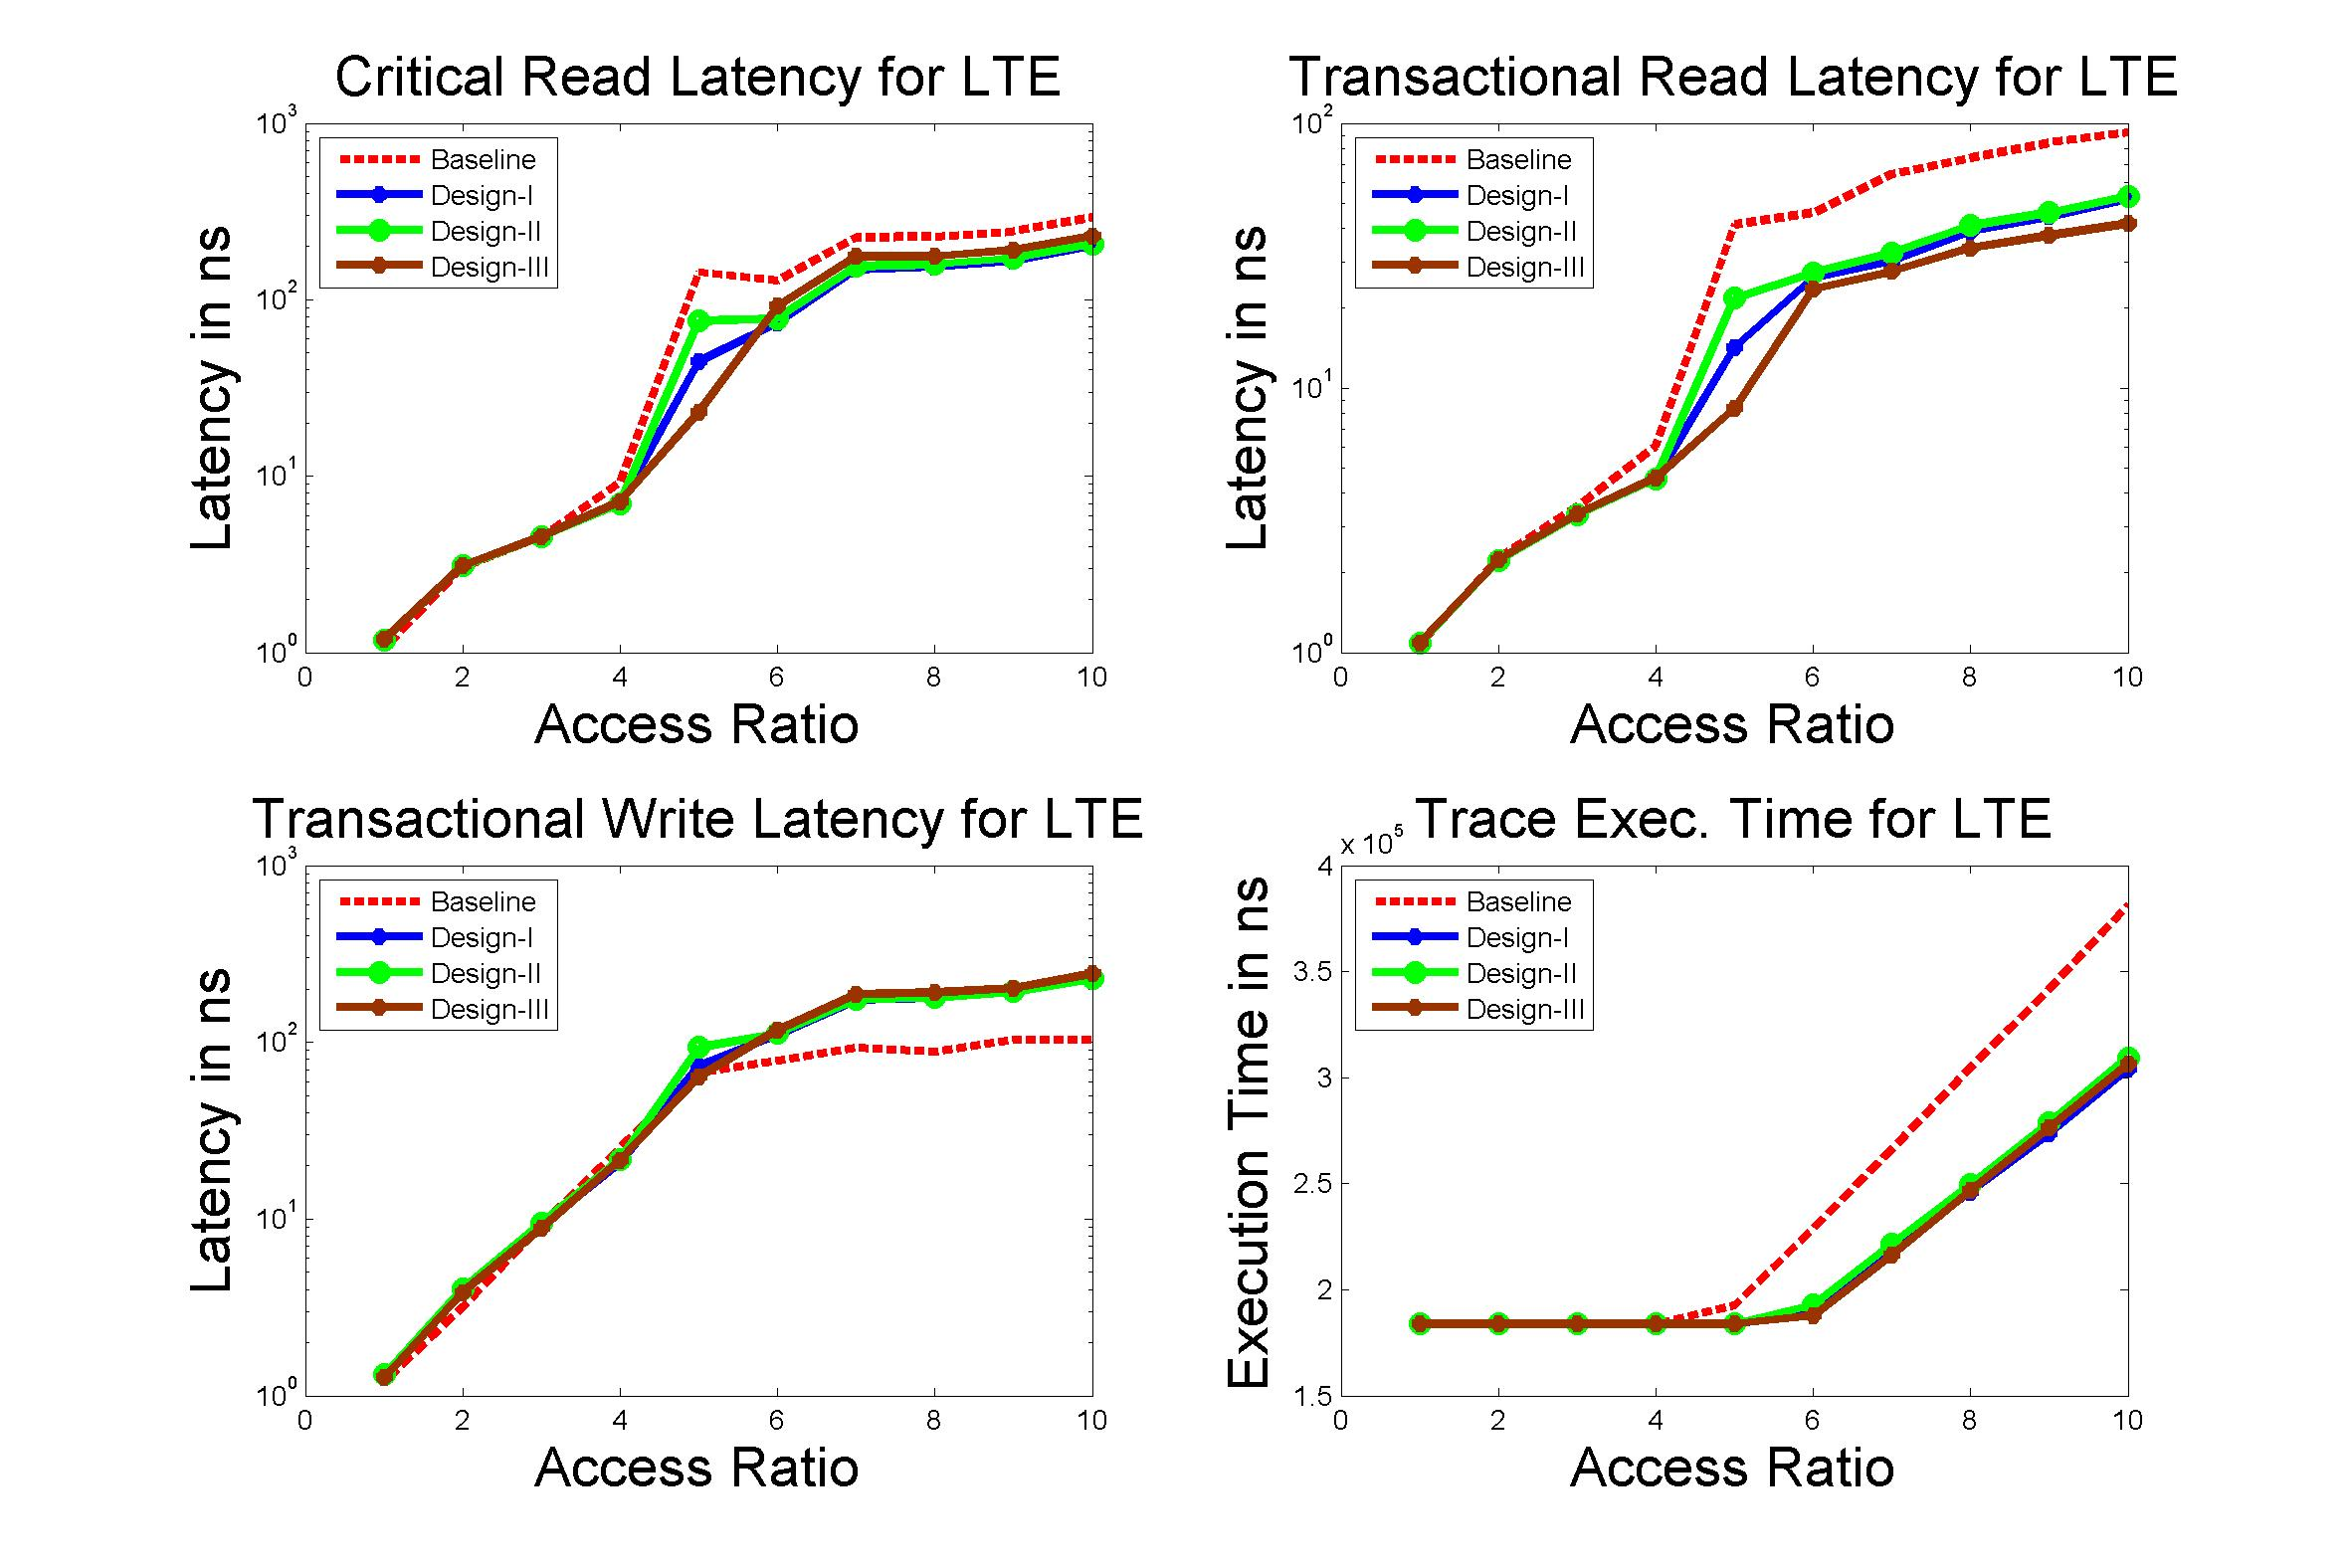
\includegraphics[width=\linewidth]{LTE.jpg}
\end{minipage}
\caption{
{\bf Performance Graphs for LTE trace} }
\label{fig:LTE}
\end{figure}
%-------------------------------------------------
\cleardoublepage
%-------------------------------------------------
\begin{figure}[htb]
%	\centering
\begin{minipage}[!t]{0.33\linewidth}
        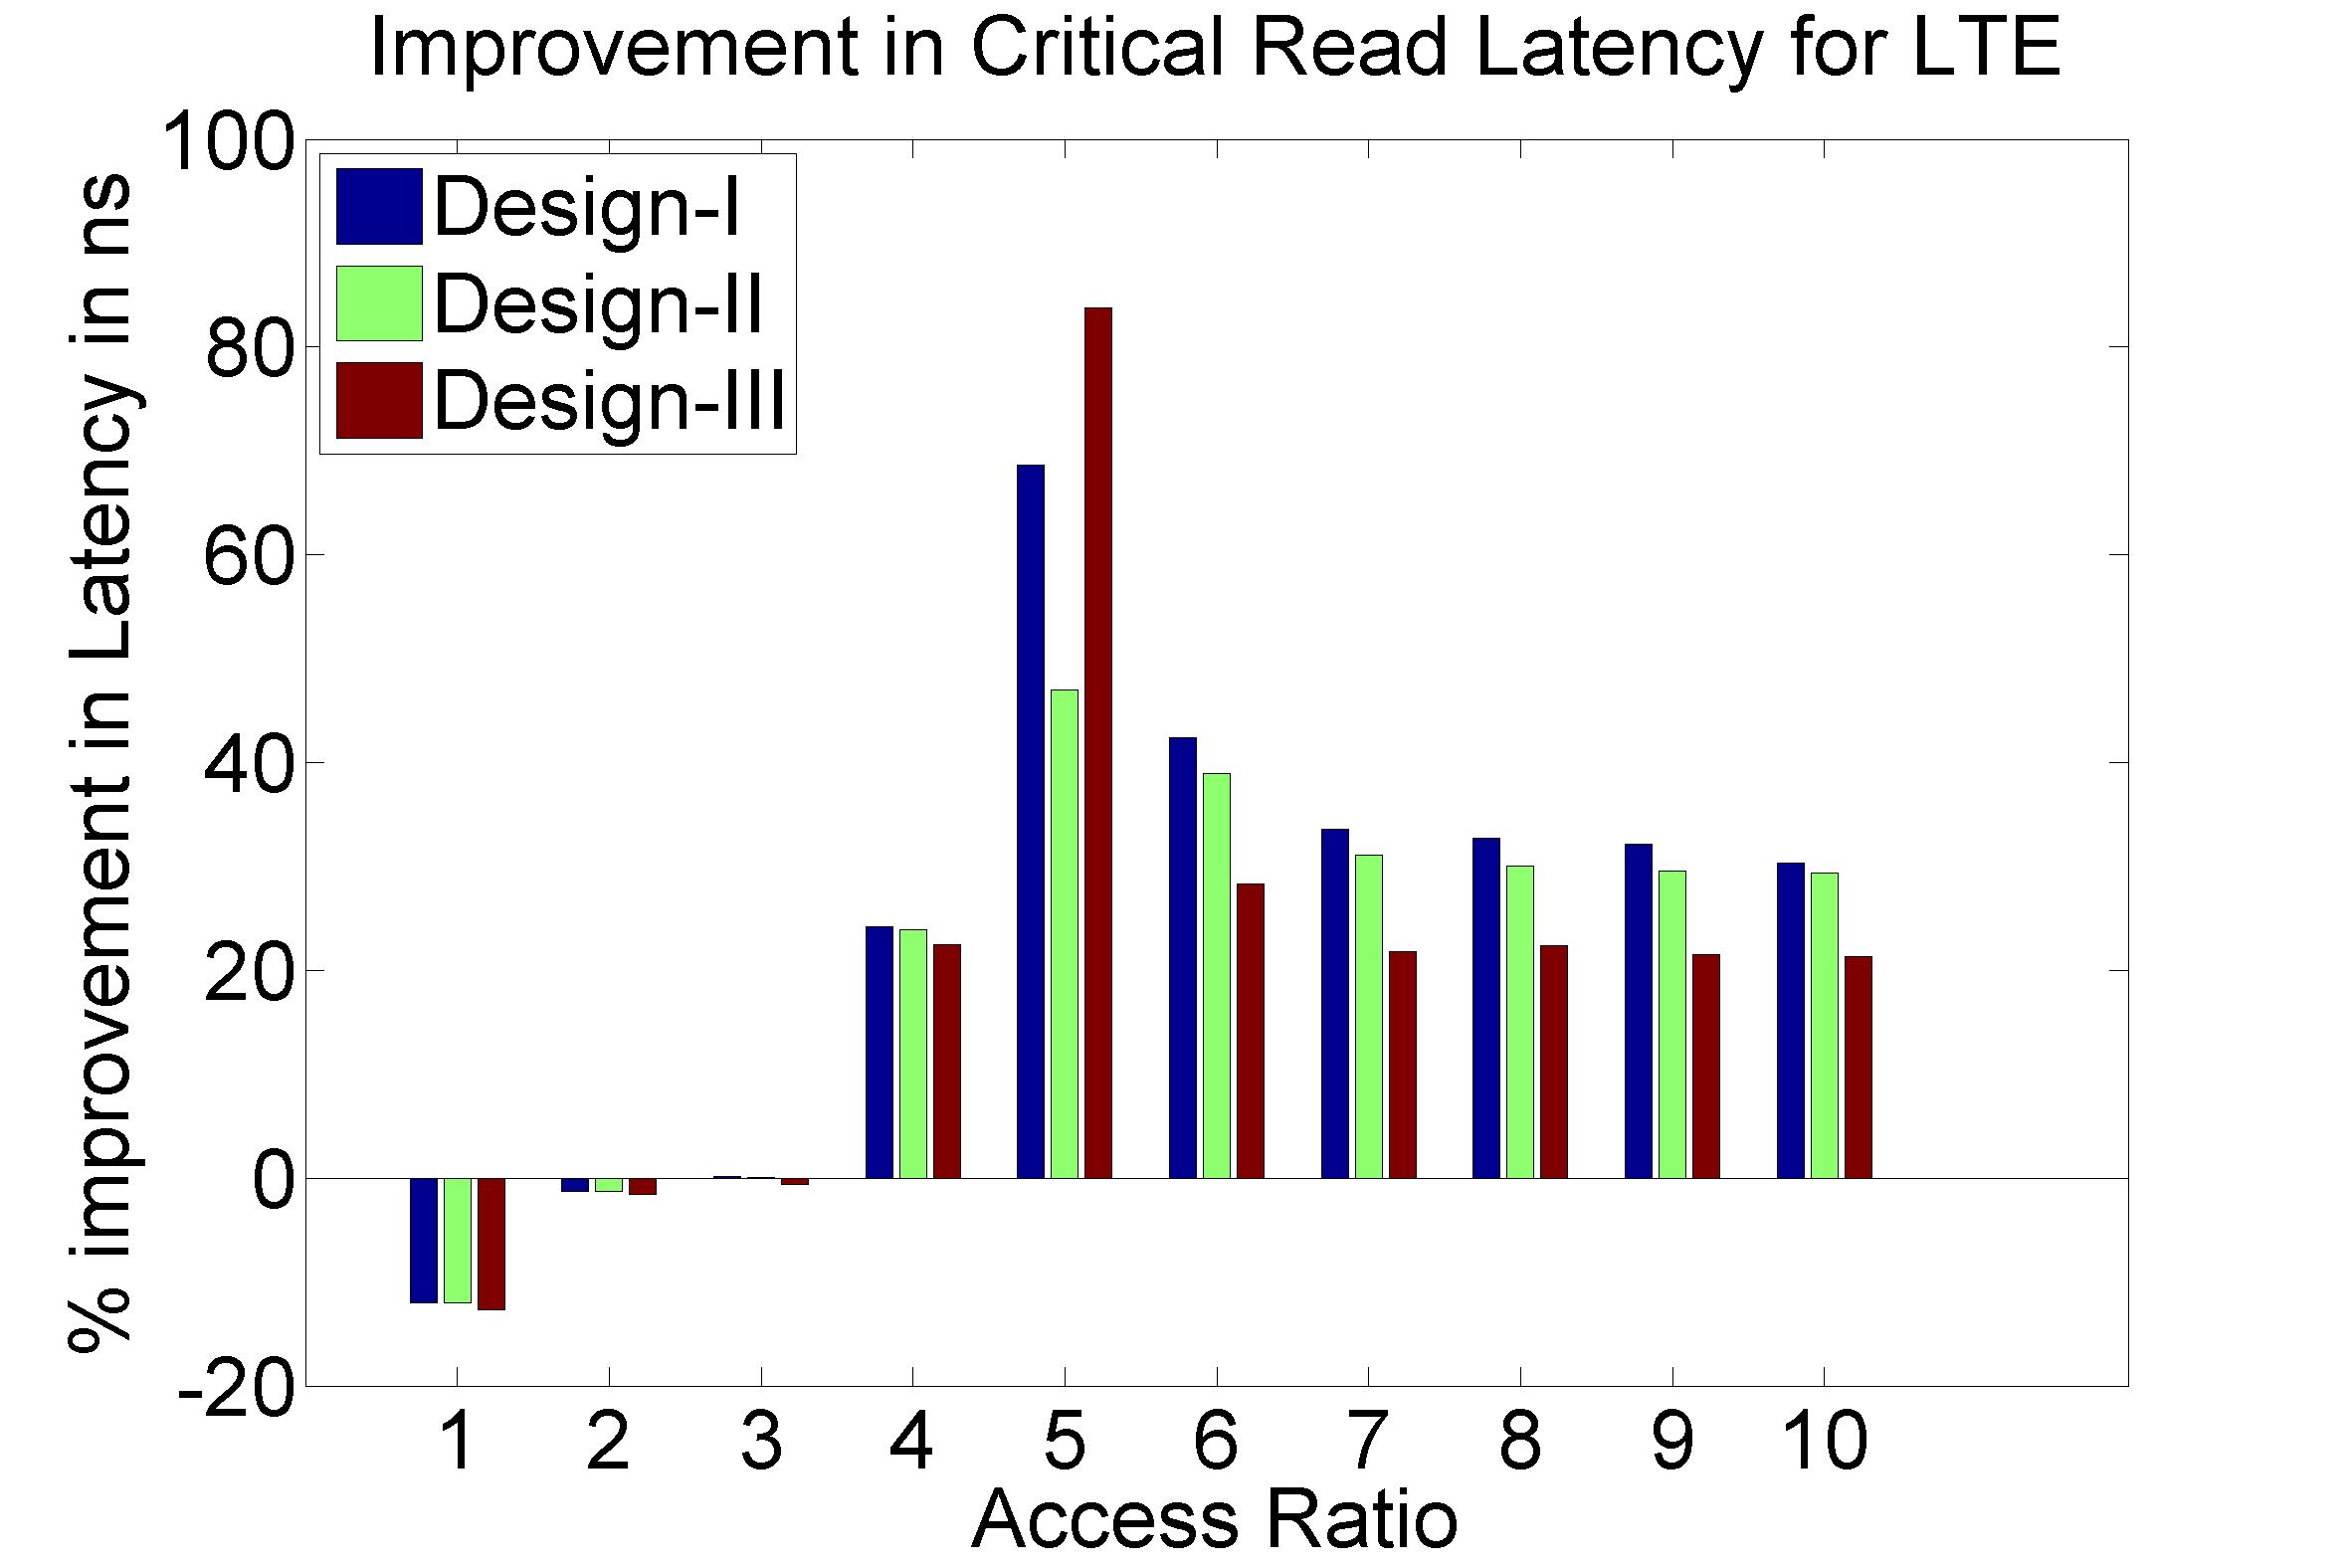
\includegraphics[width=\linewidth]{LTE_critical_latency_improvement.jpeg}
\end{minipage}
\begin{minipage}[!t]{0.33\linewidth}
        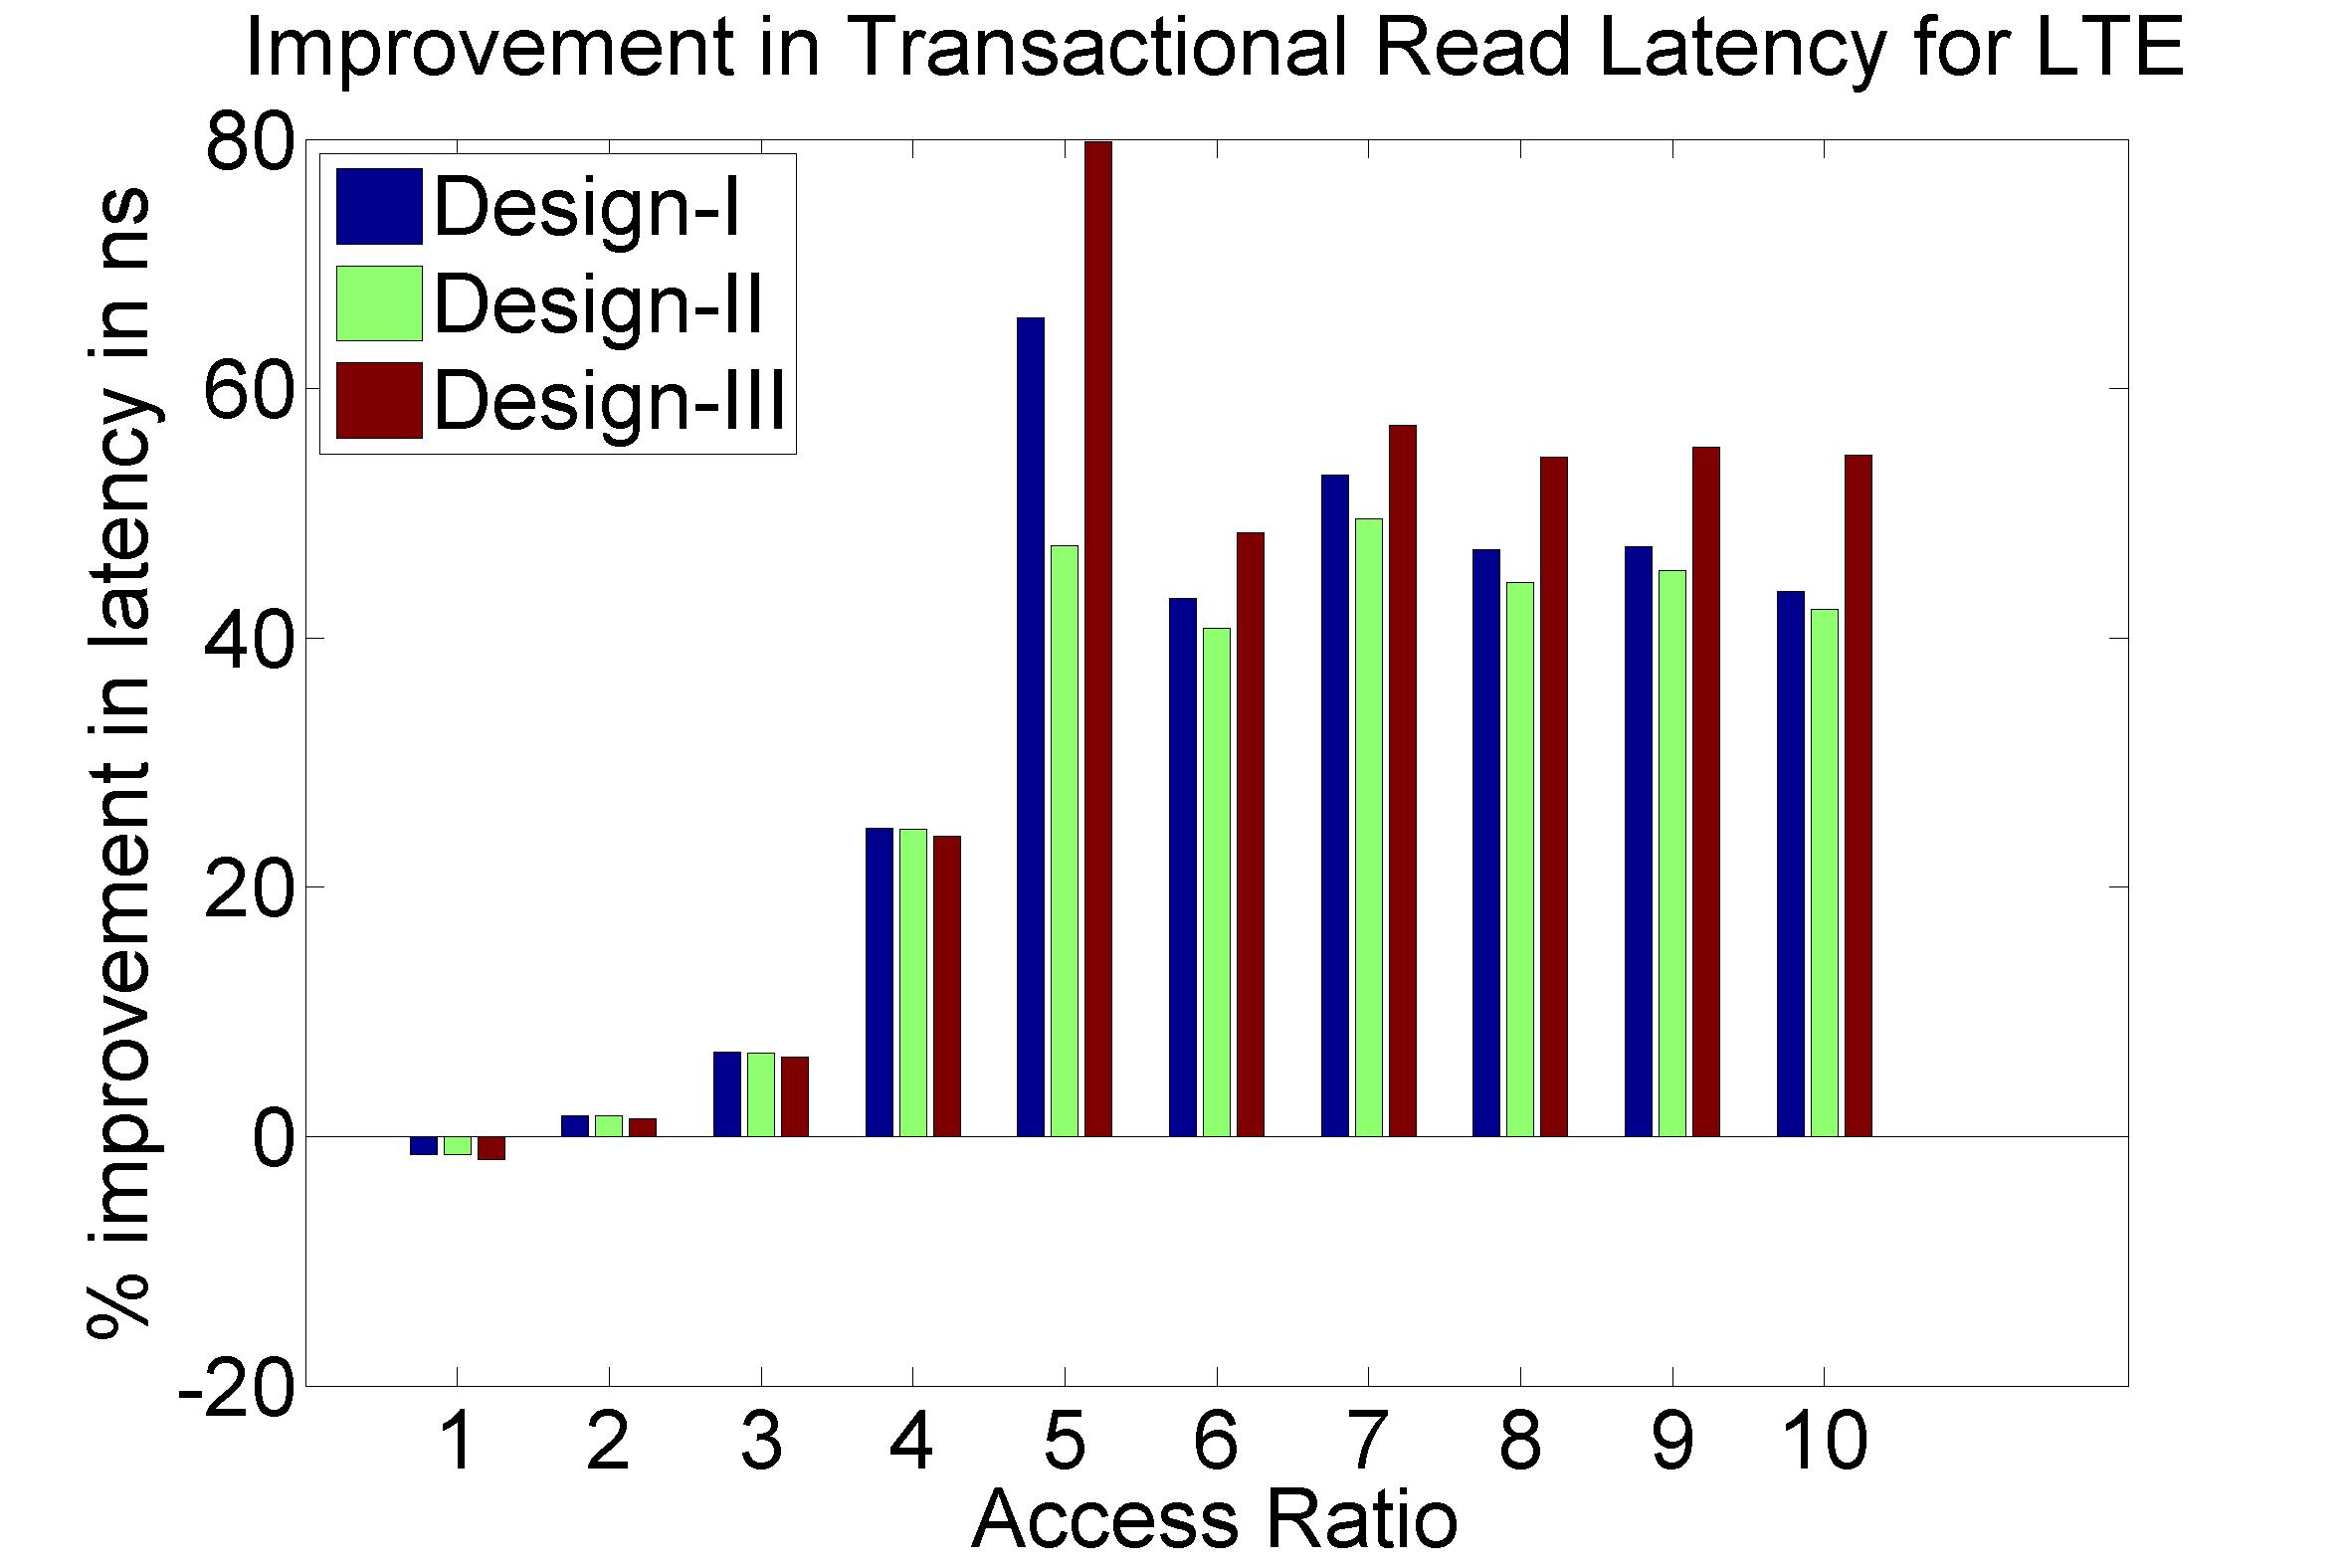
\includegraphics[width=\linewidth]{LTE_transactional_latency_improvement.jpeg}
\end{minipage}
\begin{minipage}[!t]{0.33\linewidth}
        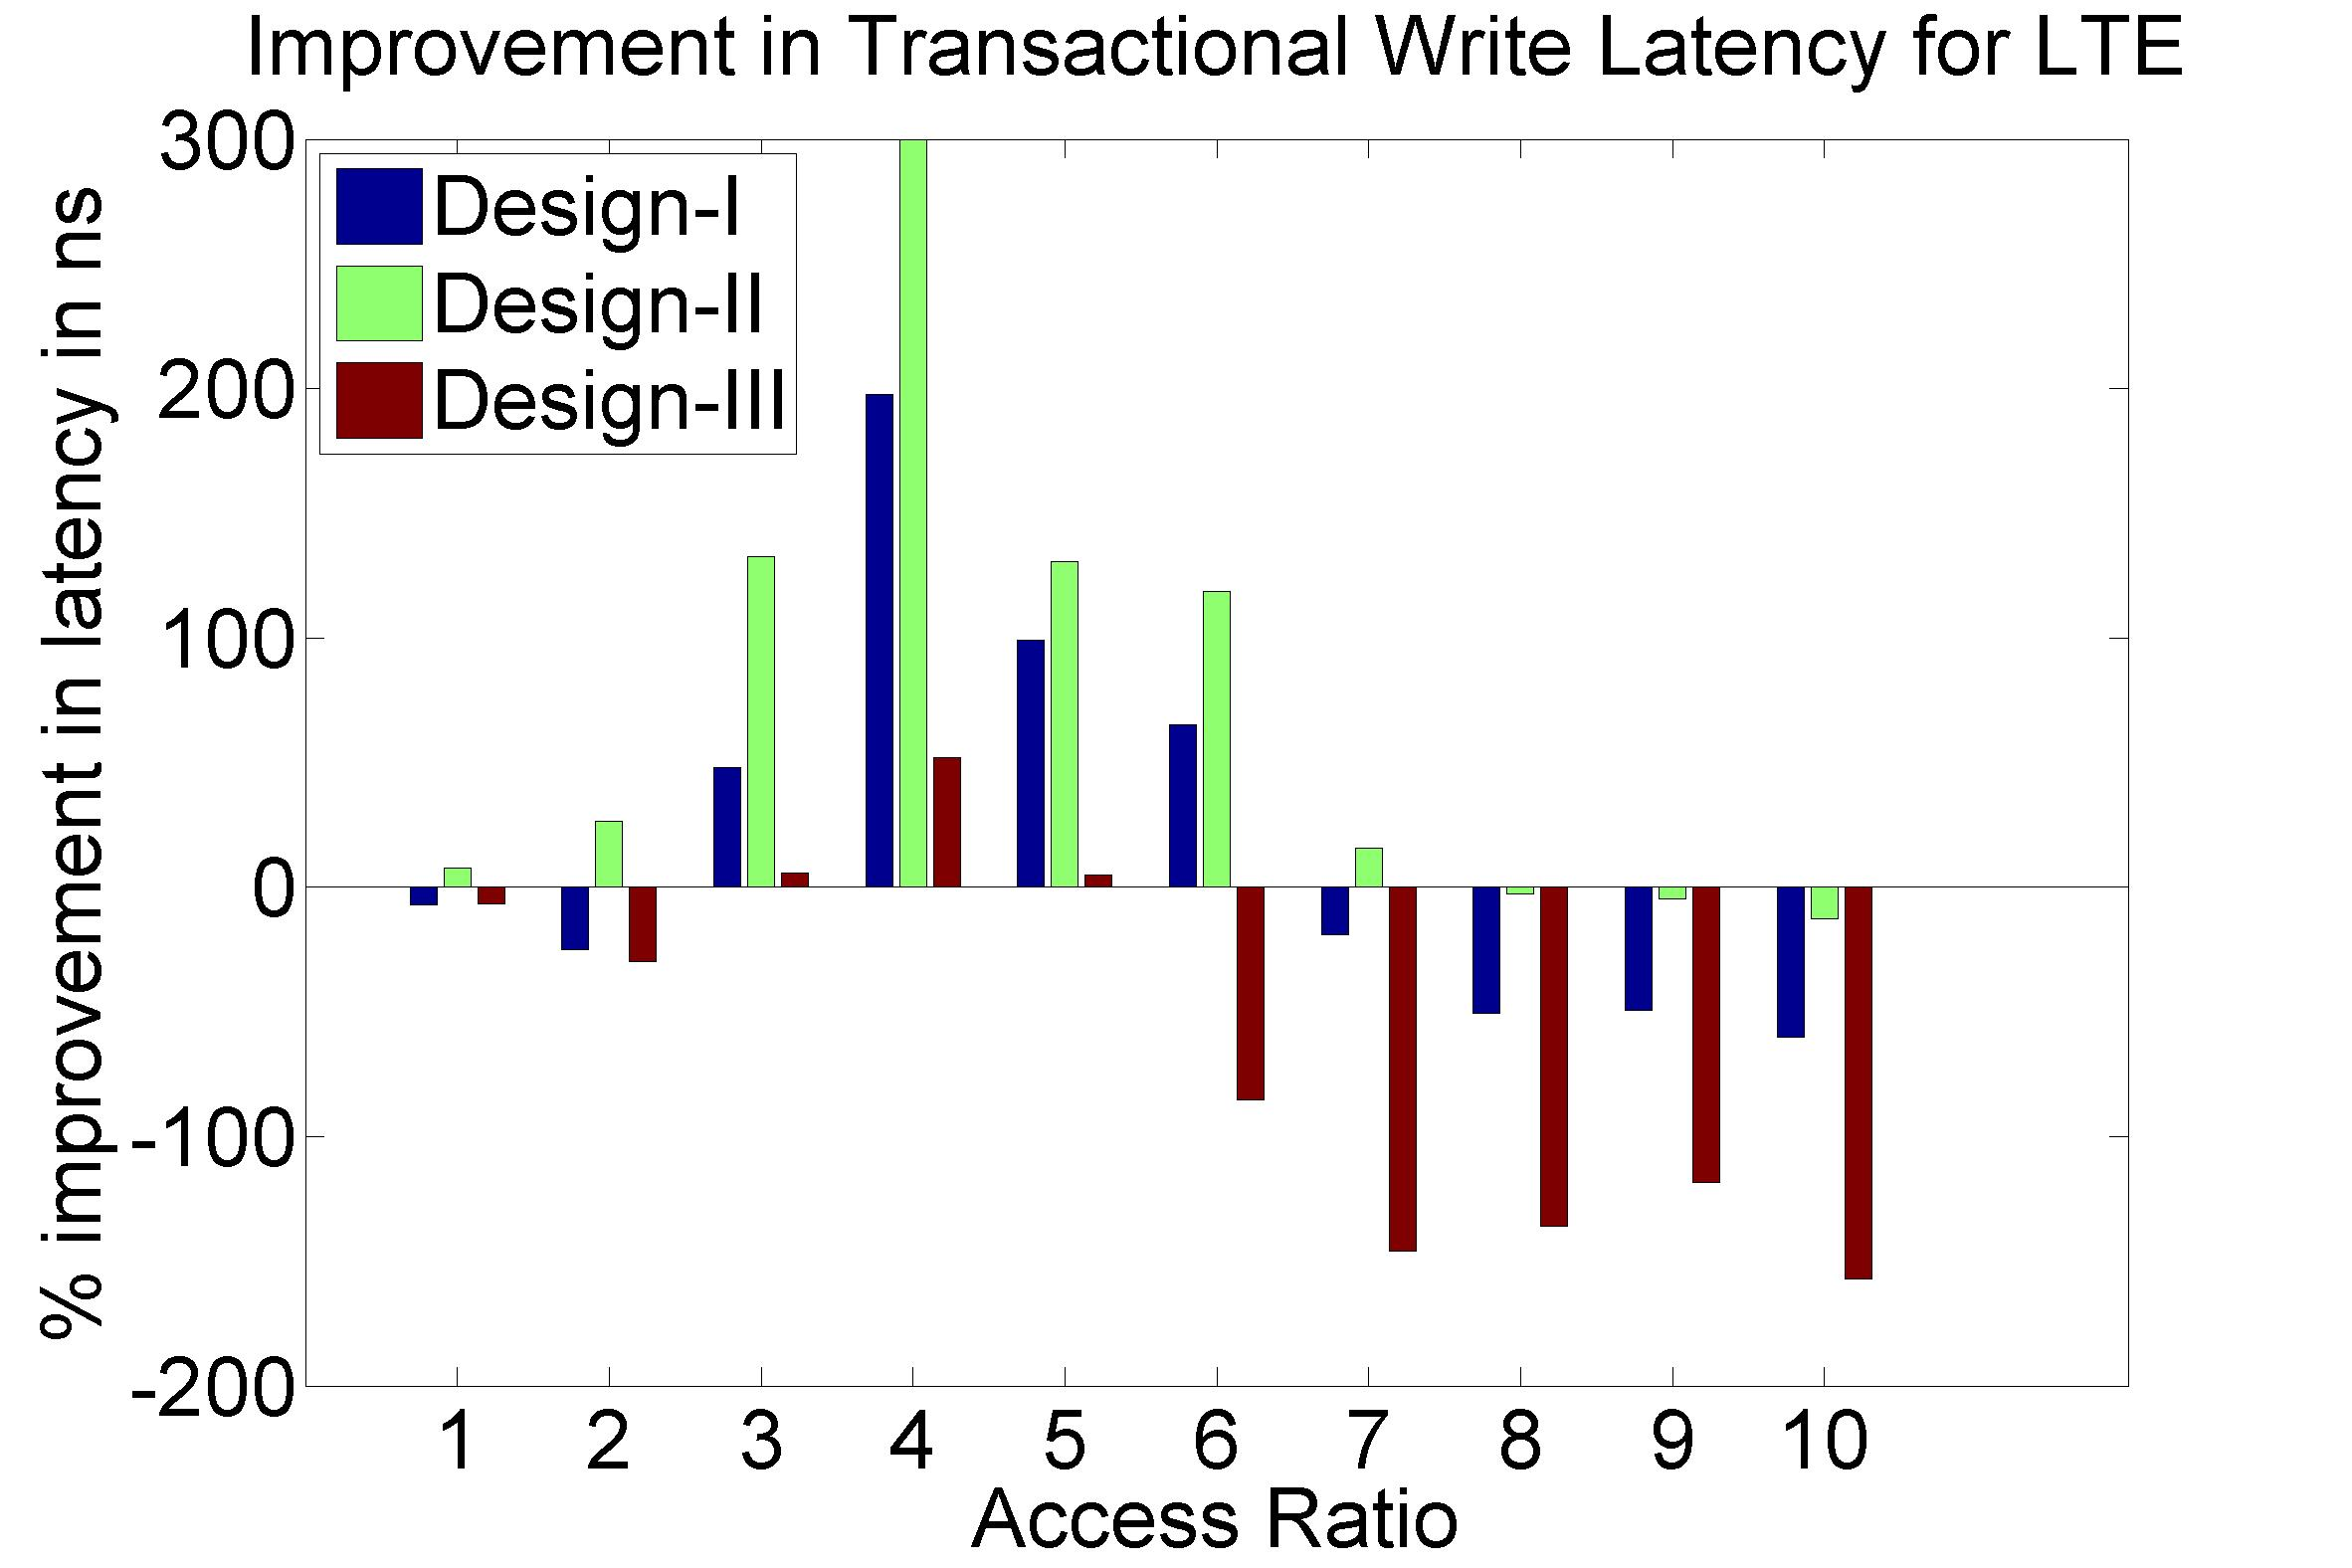
\includegraphics[width=\linewidth]{LTE_write_latency_improvement.jpeg}
\end{minipage}
\caption{
{\bf Performance Graphs for LTE trace} }
\label{fig:LTE_improvement}
\end{figure}
%-------------------------------------------------
Observations:
\begin{itemize}
	\item LTE trace is a medium density trace.
	\item The benefit for coding for read access is favourable for access ratios for 4 and more. 
	\item The write transaction latency shows improvement for access ratios of 3 to 6.
	\item The coding benefits are best at access ratio of 4, 5 and 6.
\end{itemize}
\cleardoublepage
%-------------------------------------------------
\begin{figure}[htb]
\begin{minipage}[!t]{\linewidth}
        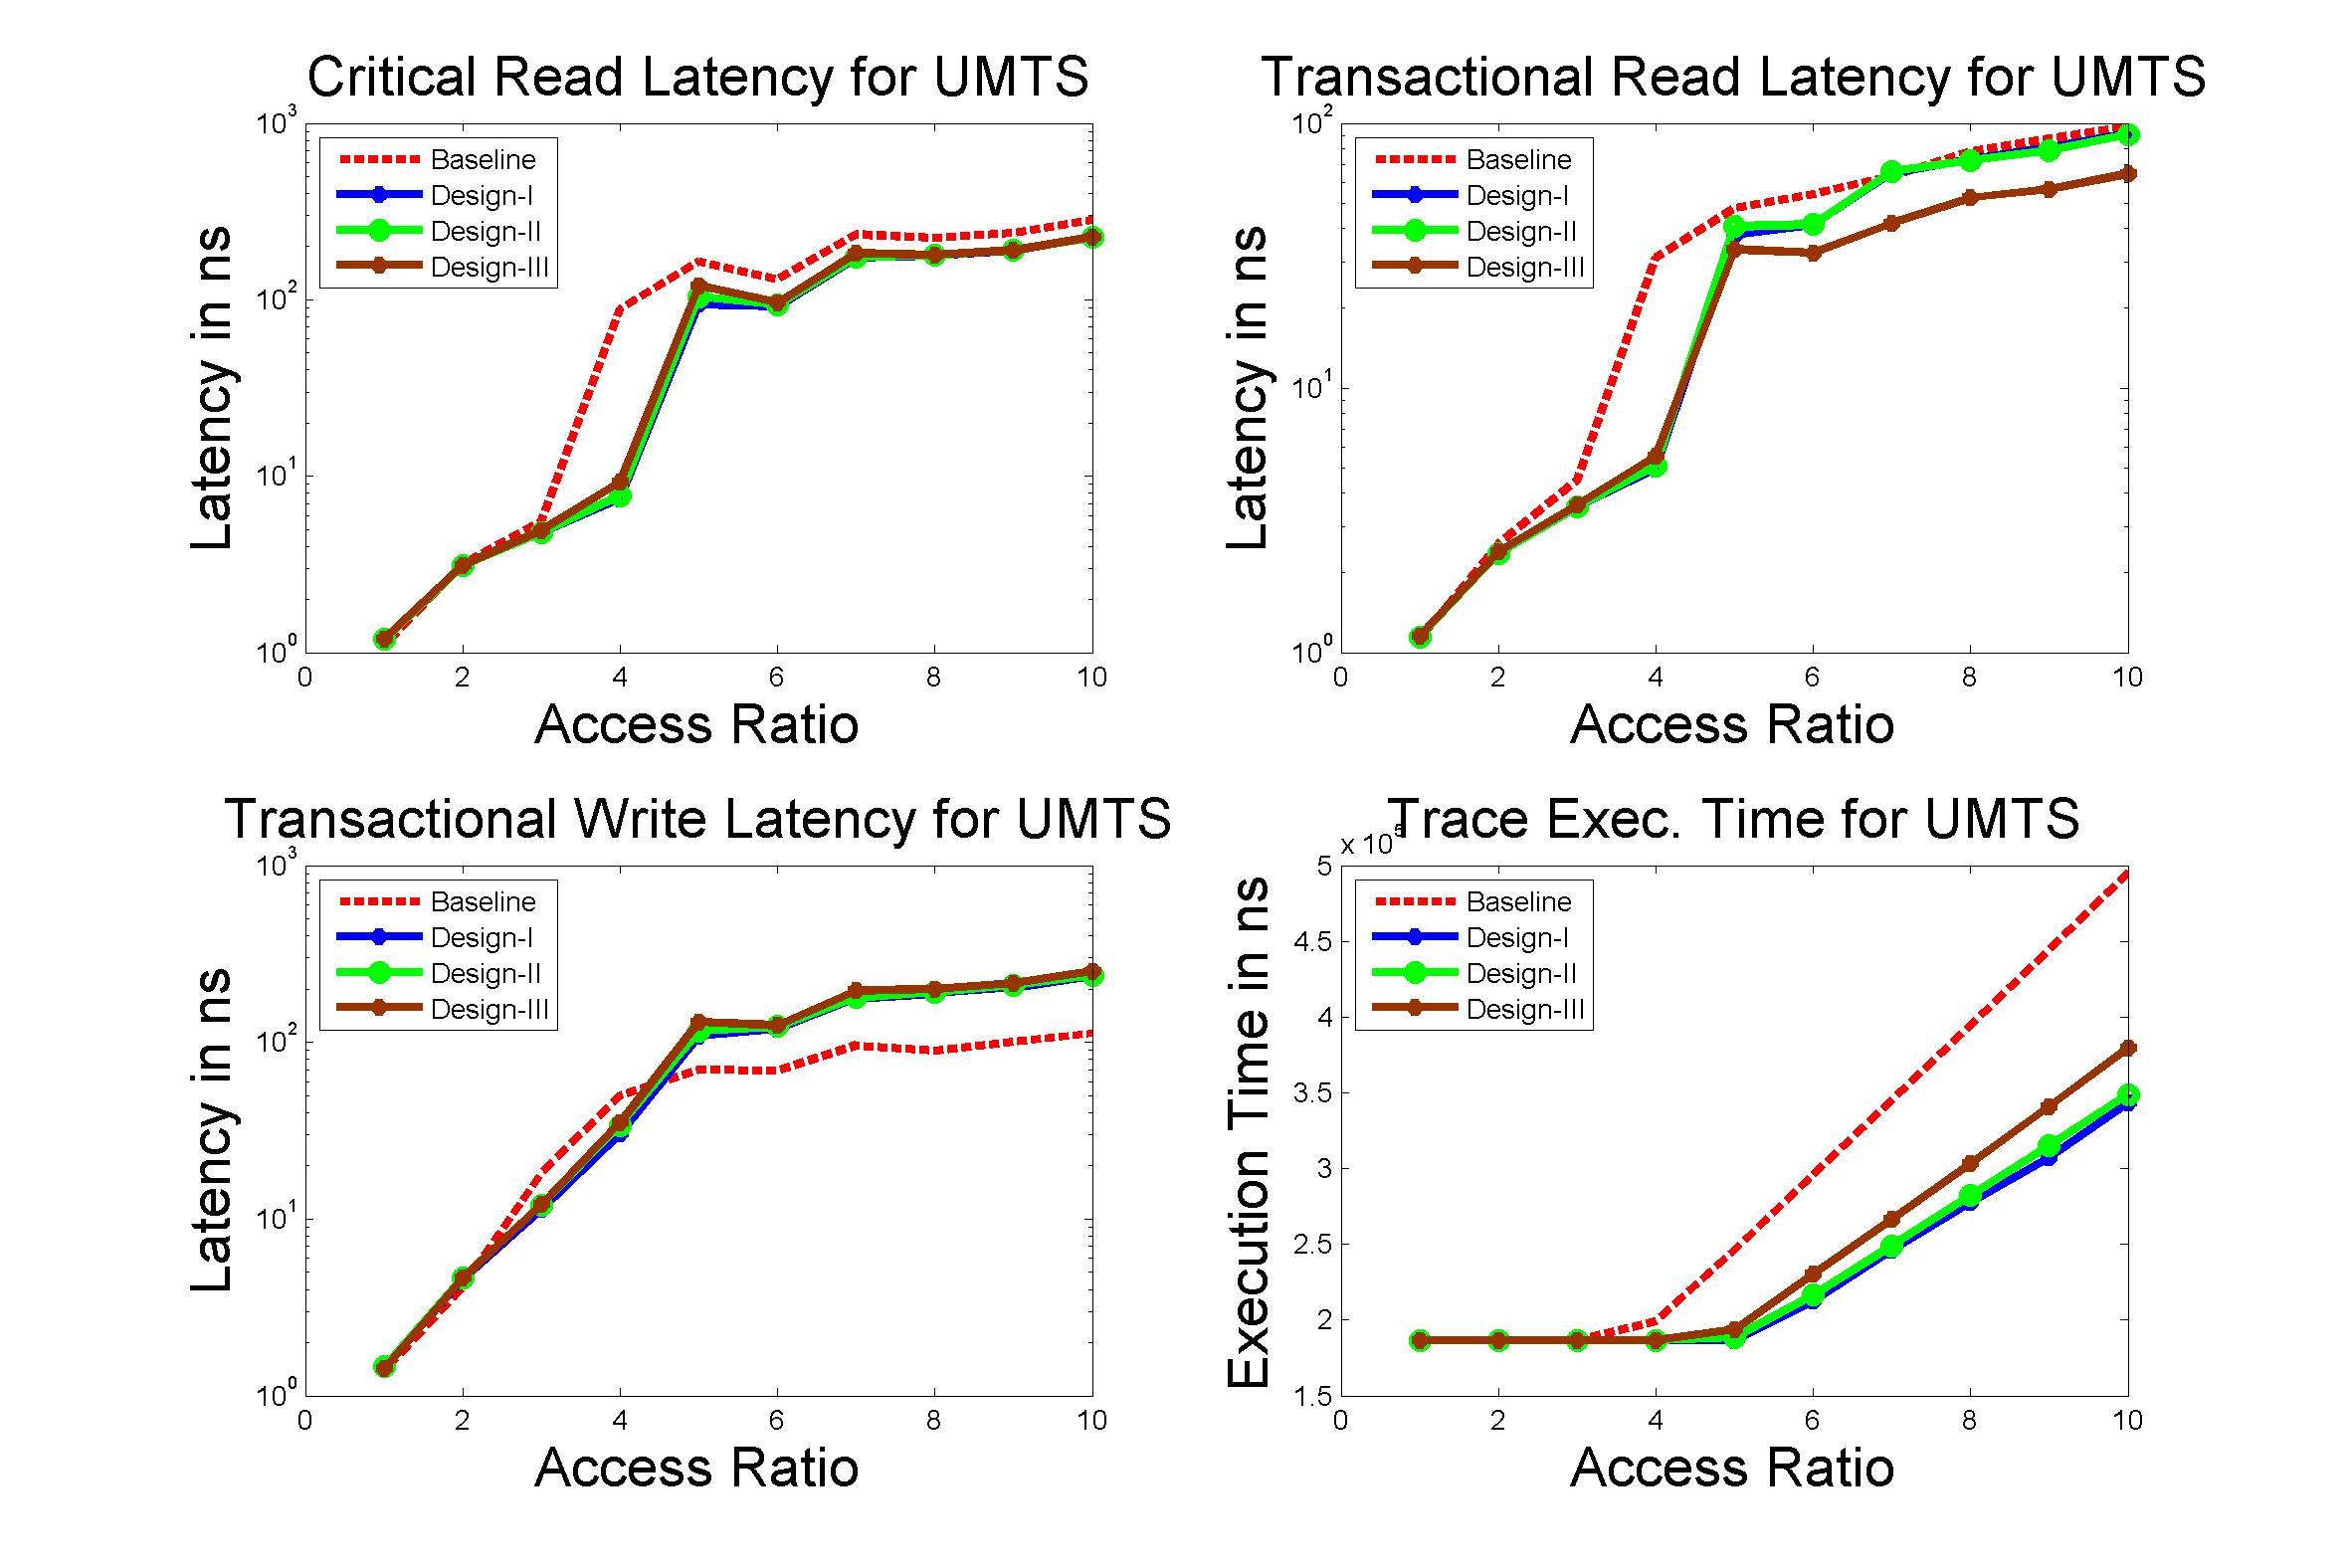
\includegraphics[width=\linewidth]{UMTS.jpg}
\end{minipage}
\caption{
{\bf Performance Graphs for UMTS trace} }
\label{fig:LTE}
\end{figure}
%-------------------------------------------------
\cleardoublepage
%-------------------------------------------------
\begin{figure}[htb]
\begin{minipage}[!t]{0.33\linewidth}
        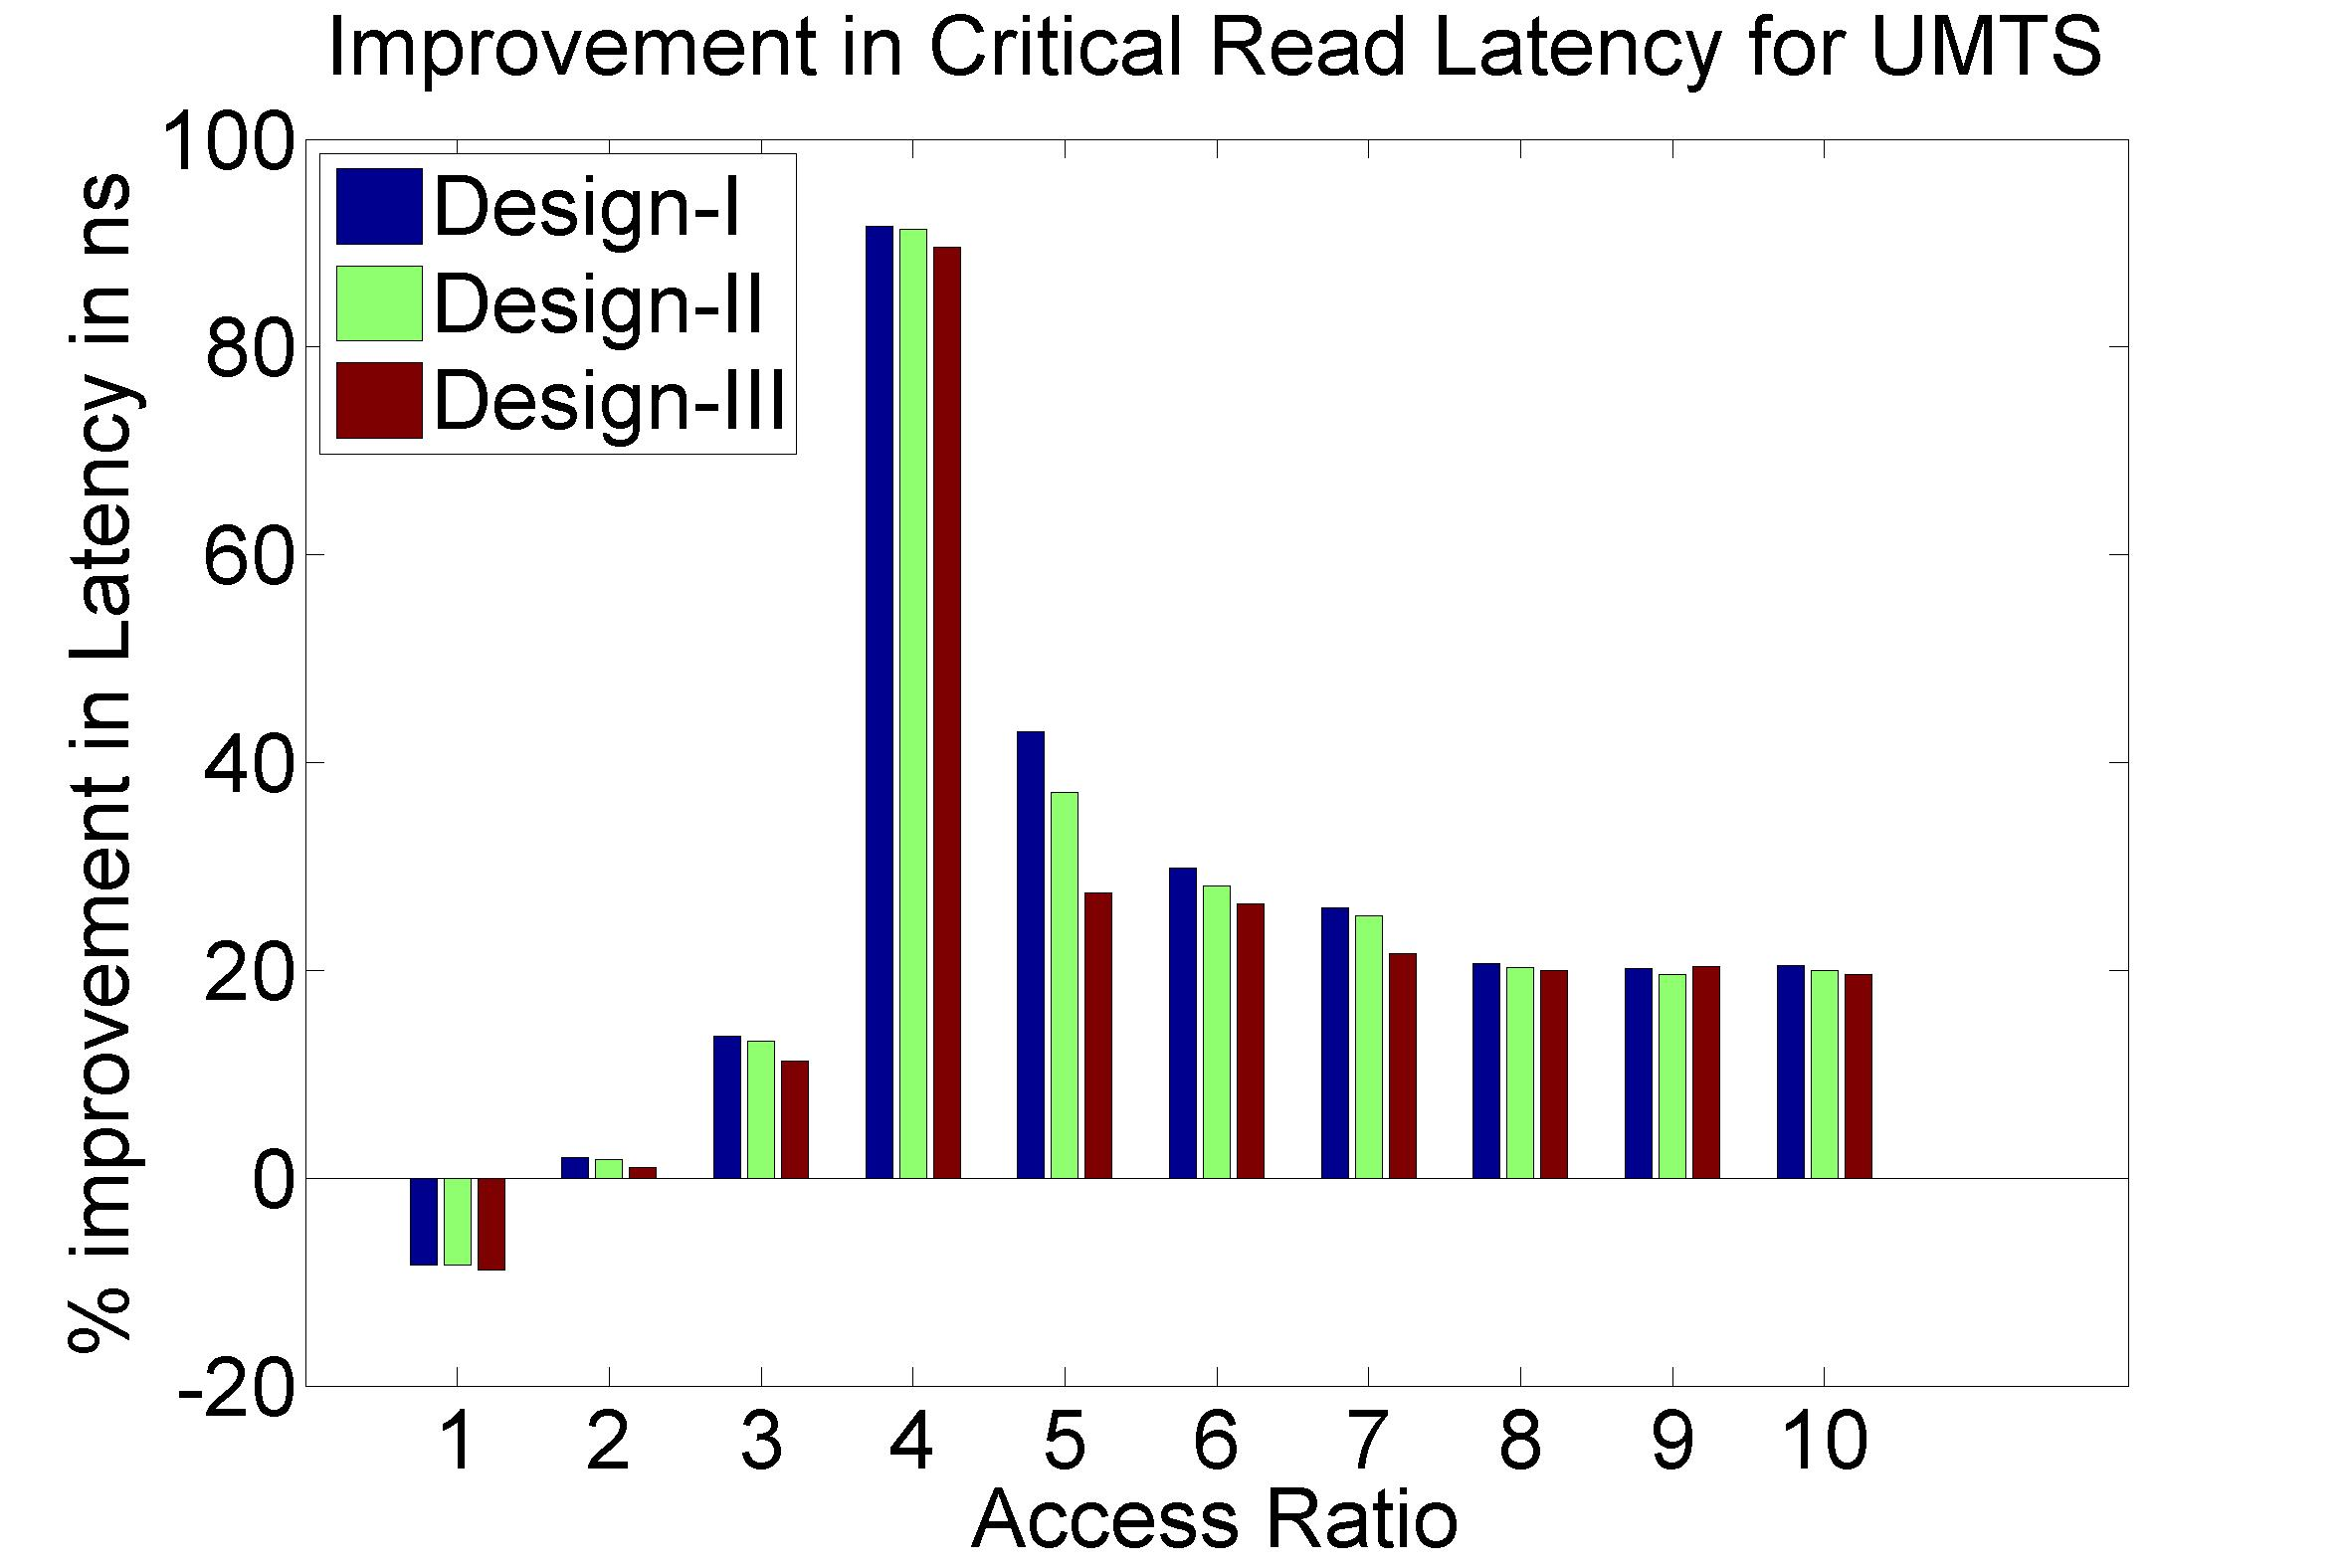
\includegraphics[width=\linewidth]{UMTS_critical_latency_improvement.jpeg}
\end{minipage}
\begin{minipage}[!t]{0.33\linewidth}
        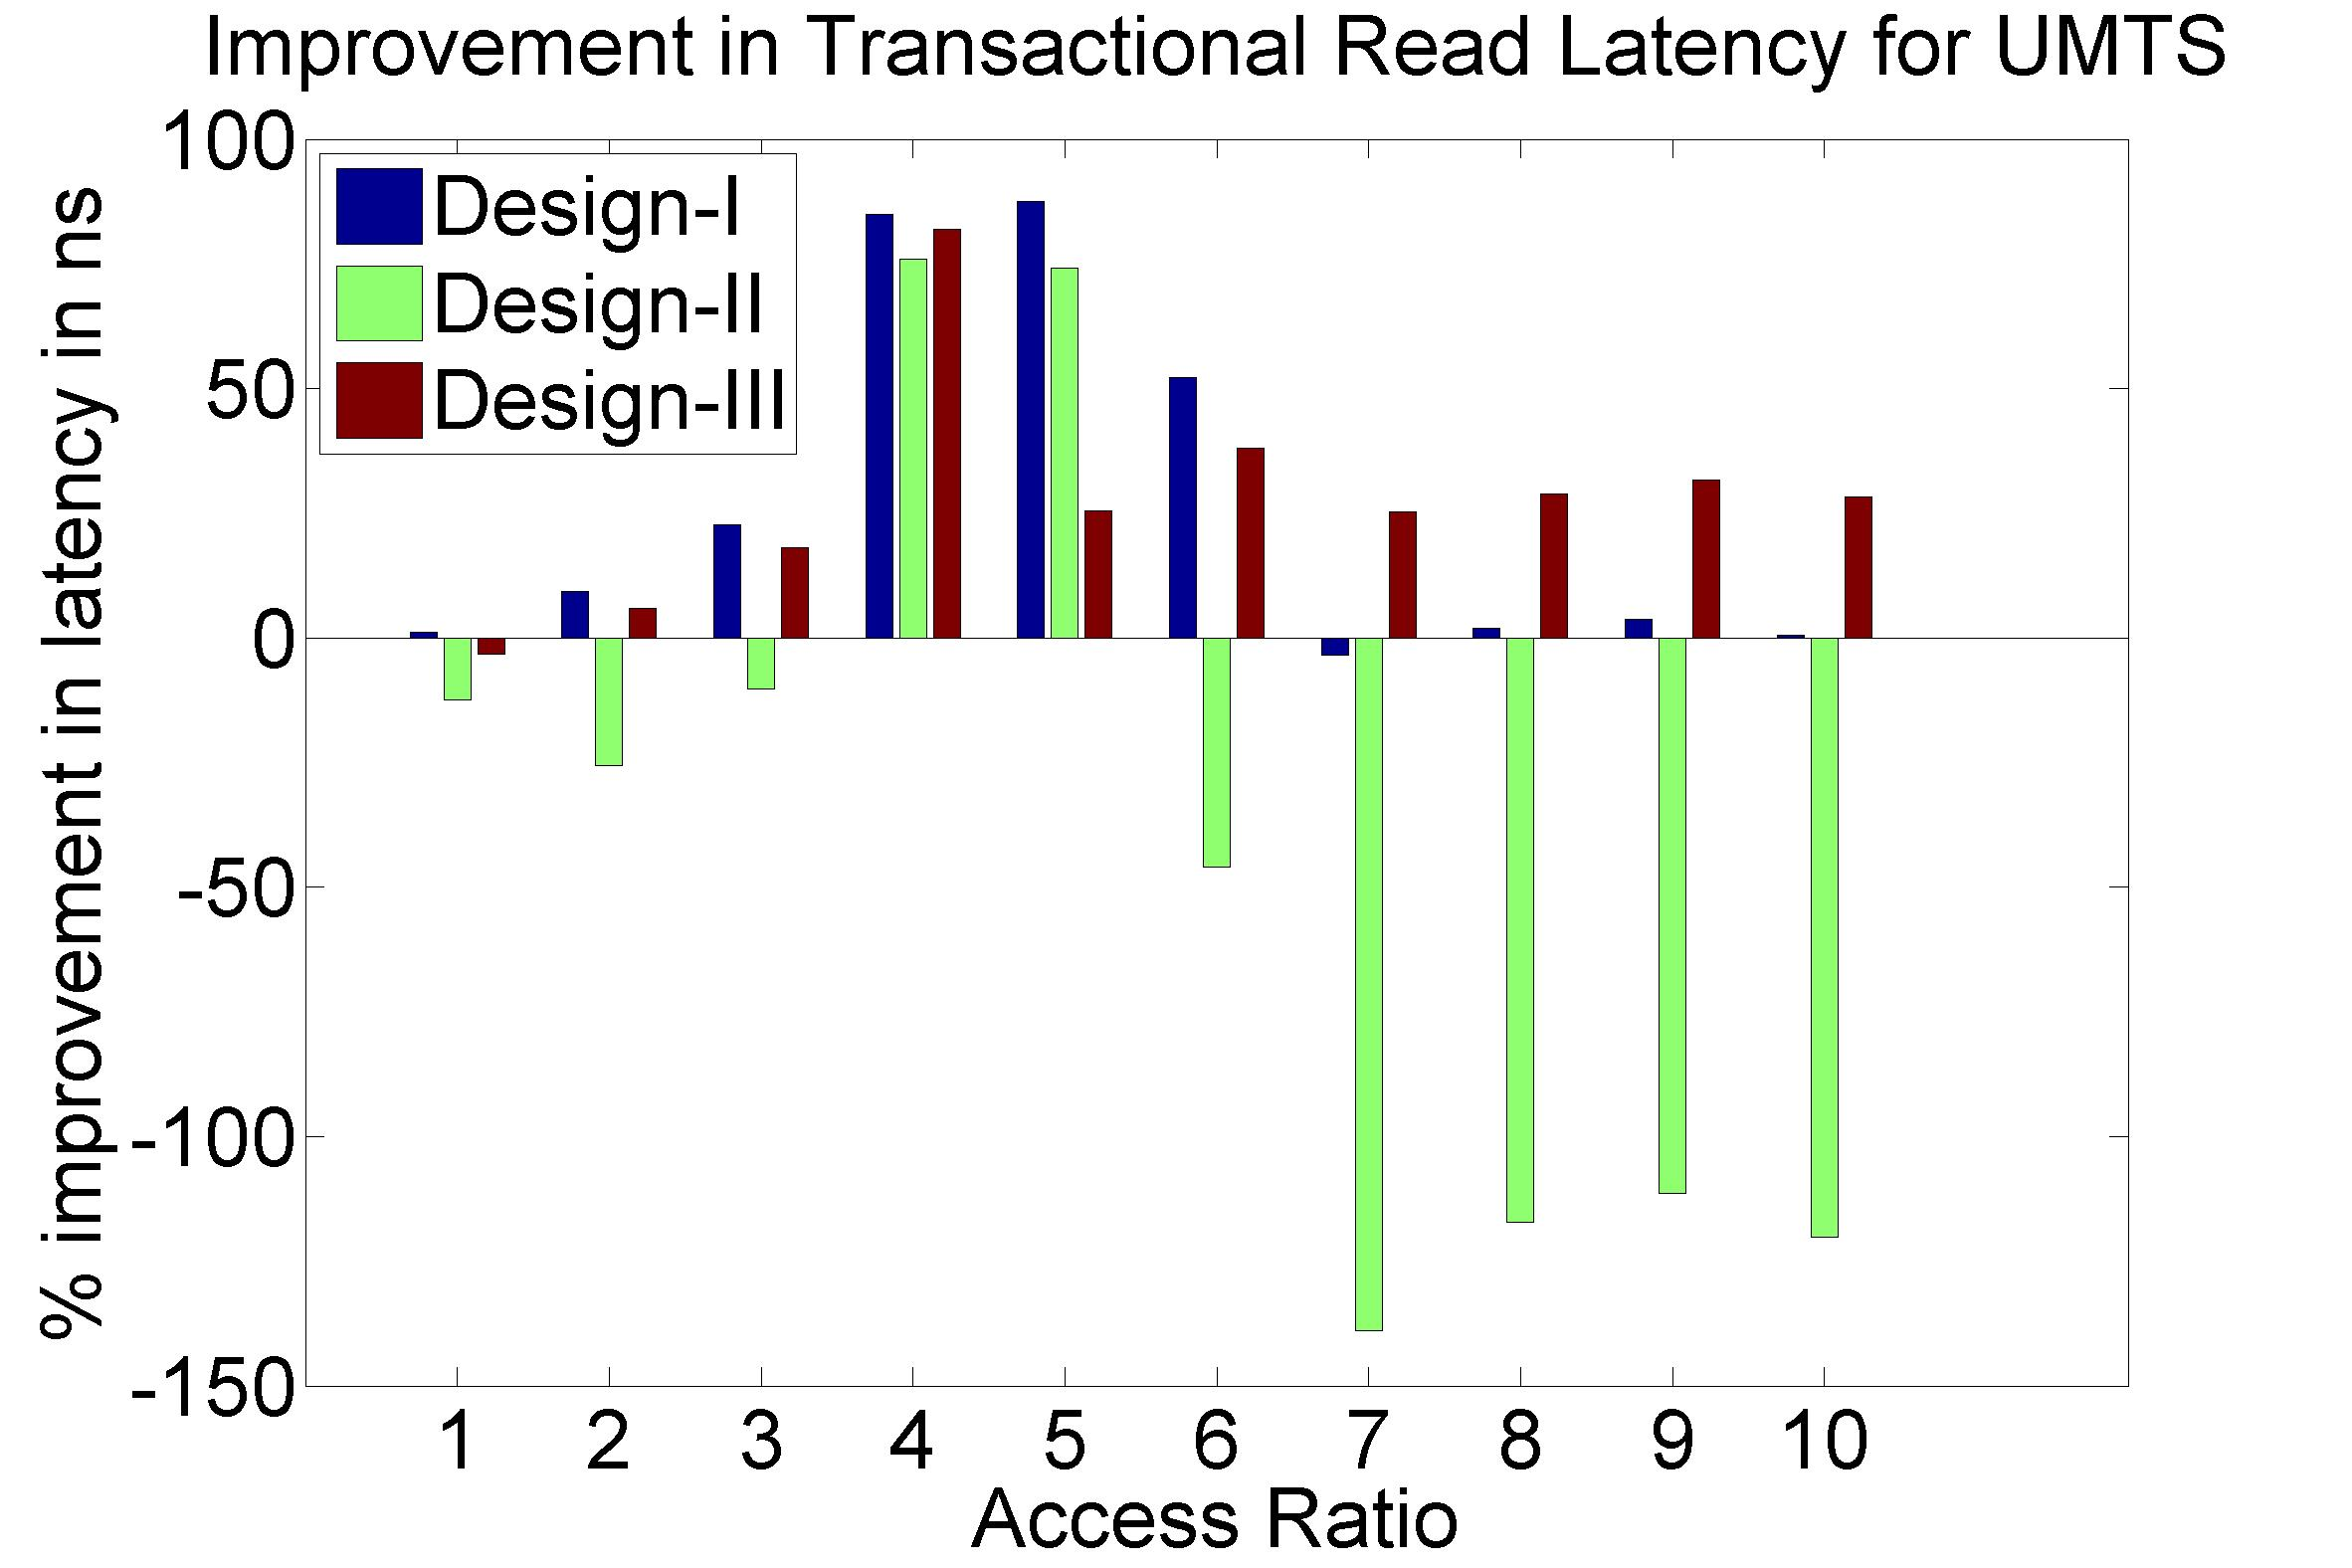
\includegraphics[width=\linewidth]{UMTS_transactional_latency_improvement.jpeg}
\end{minipage}
\begin{minipage}[!t]{0.33\linewidth}
        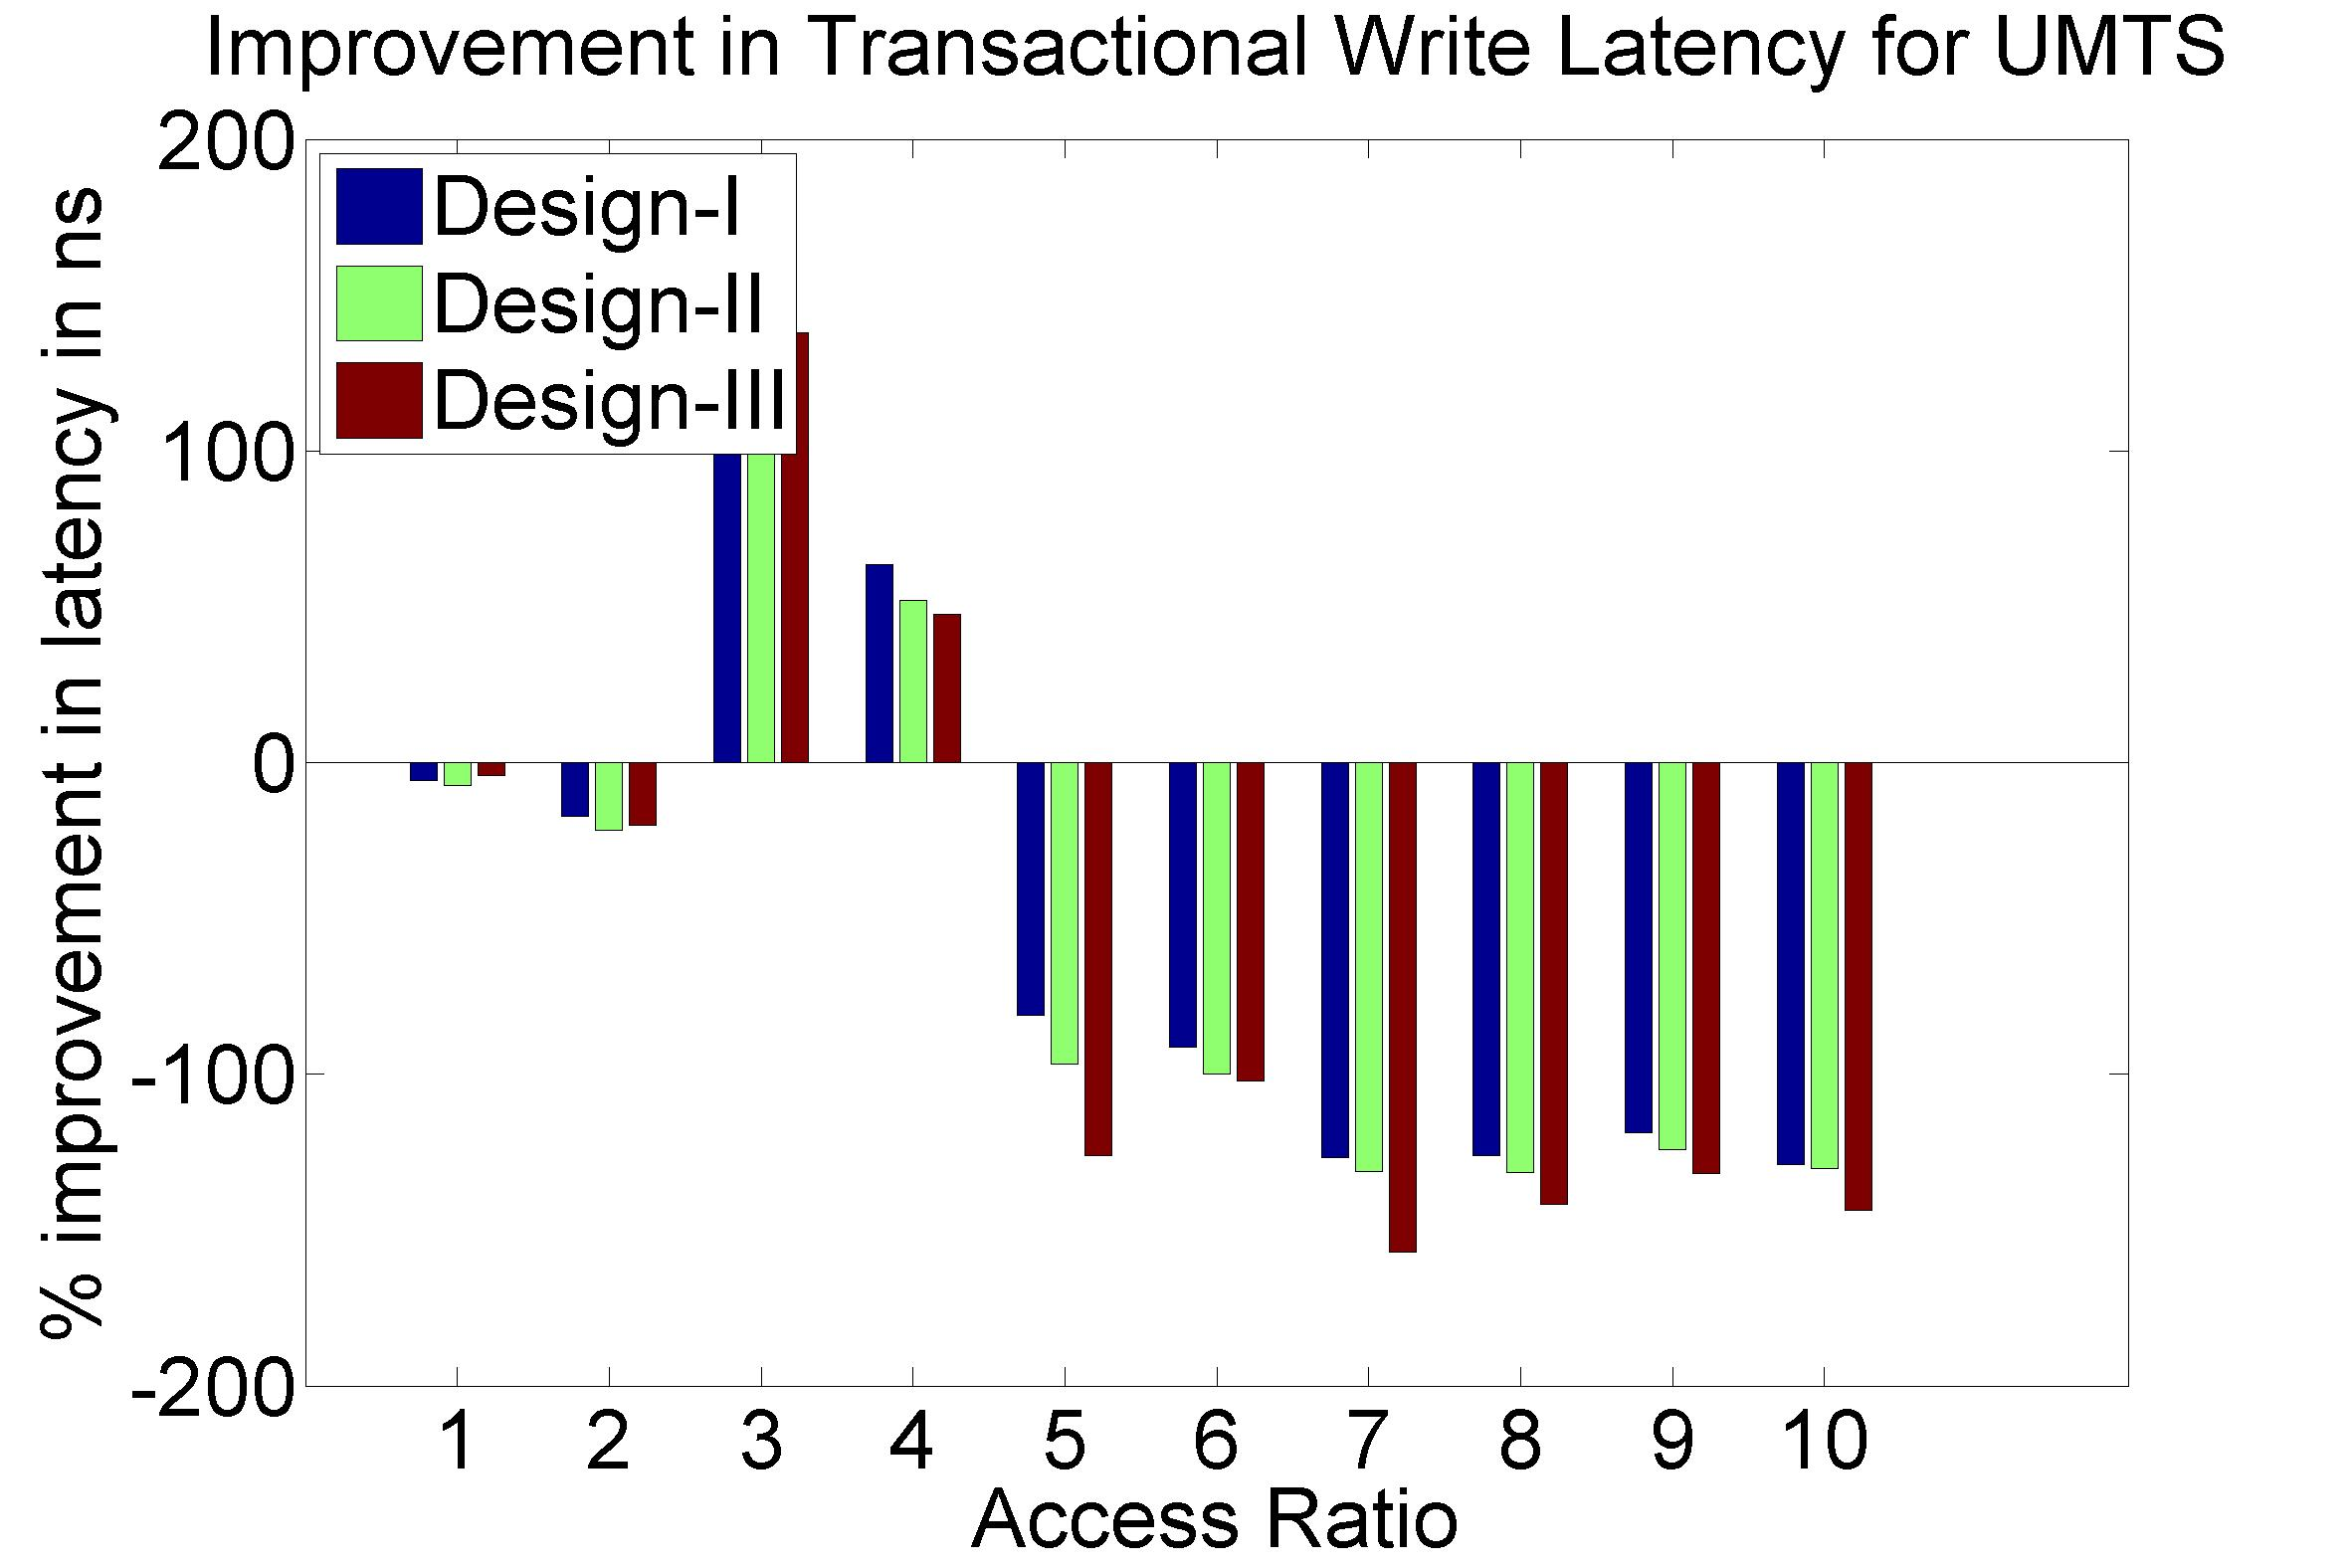
\includegraphics[width=\linewidth]{UMTS_write_latency_improvement.jpeg}
\end{minipage}
\caption{
{\bf Performance Graphs for UMTS trace} }
\label{fig:UMTS_improvement}
\end{figure}
%-------------------------------------------------
Observations:
\begin{itemize}
	\item The UMTS trace is also a medium access trace. 
	\item The read latency improvement in UMTS is substantial for all access ratios in case of critical latency. 
	\item The Transactional Latency improvees untill access ratio of 6.
	\item The design II sees degradation in performance for higher access ratios. 
	\item Write Latency improvement is observed for access ratio of 3 and 4.
	\item The coding benefits are best at access ratio of 4.
\end{itemize}
\cleardoublepage
%-------------------------------------------------
\begin{figure}[htb]
\begin{minipage}[!t]{\linewidth}
        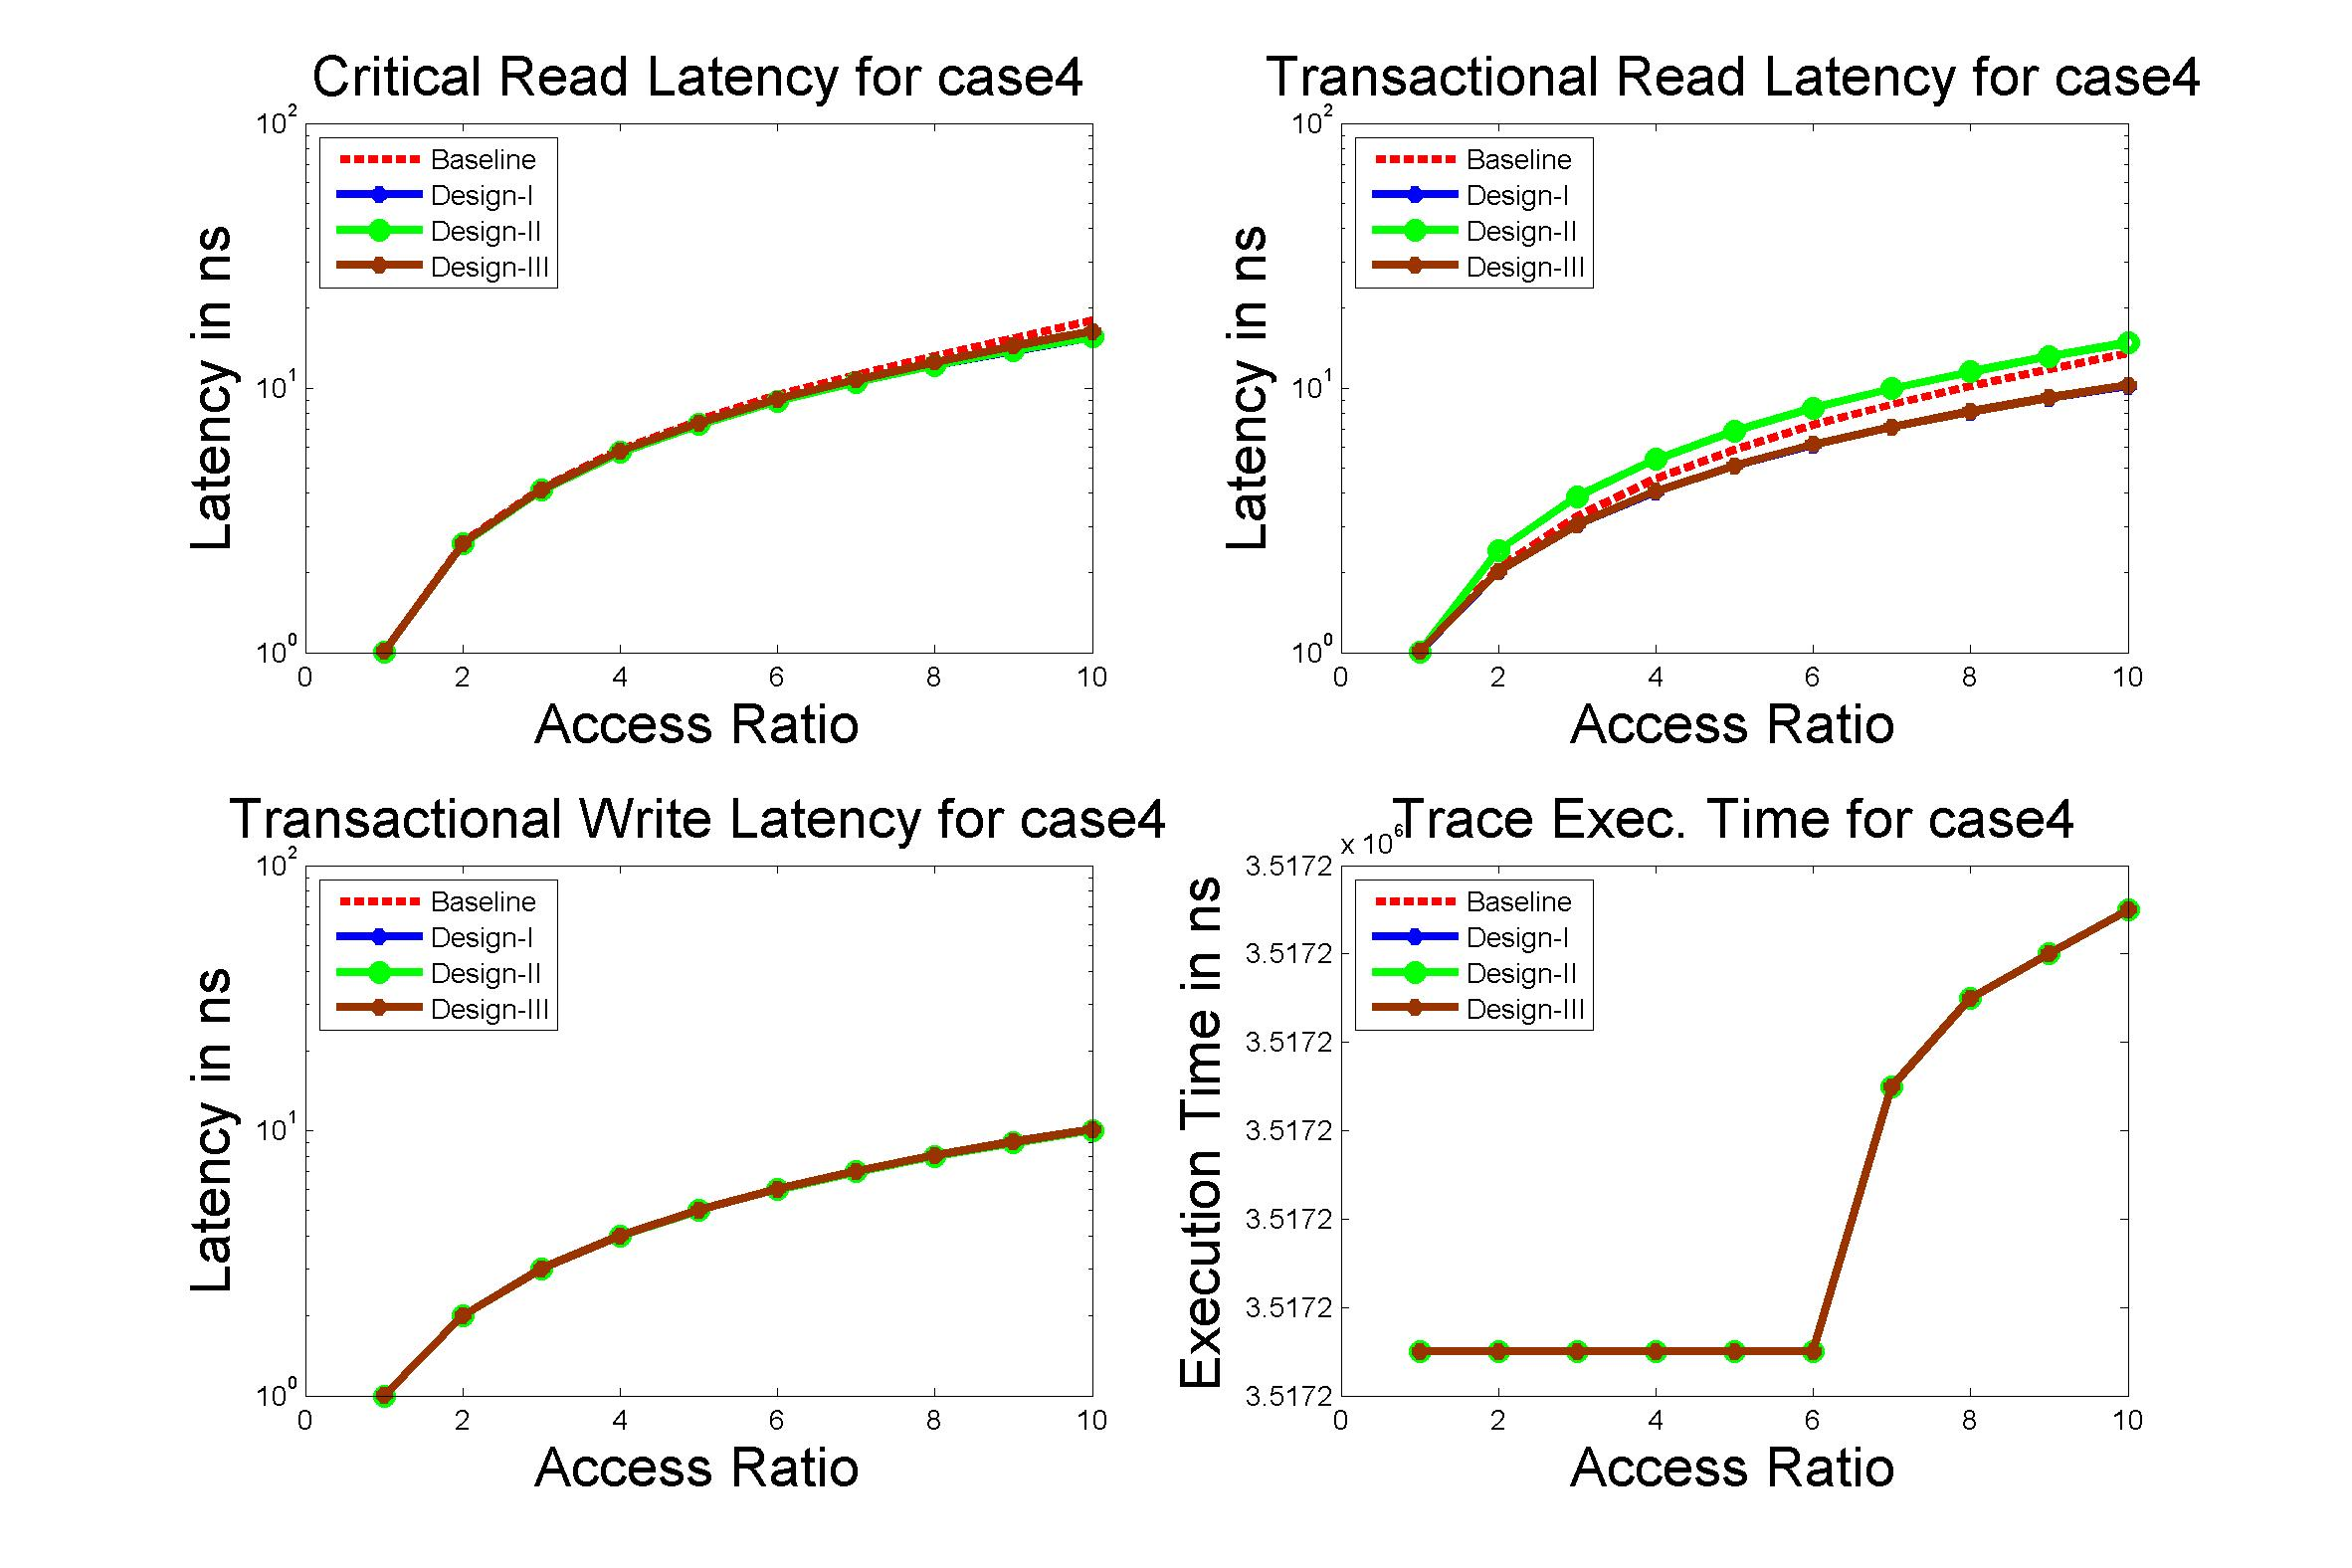
\includegraphics[width=\linewidth]{case4.jpg}
\end{minipage}
\caption{
{\bf Performance Graphs for case4 trace} }
\label{fig:case4}
\end{figure}
%-------------------------------------------------
\cleardoublepage
%-------------------------------------------------
\begin{figure}[htb]
\begin{minipage}[!t]{0.33\linewidth}
        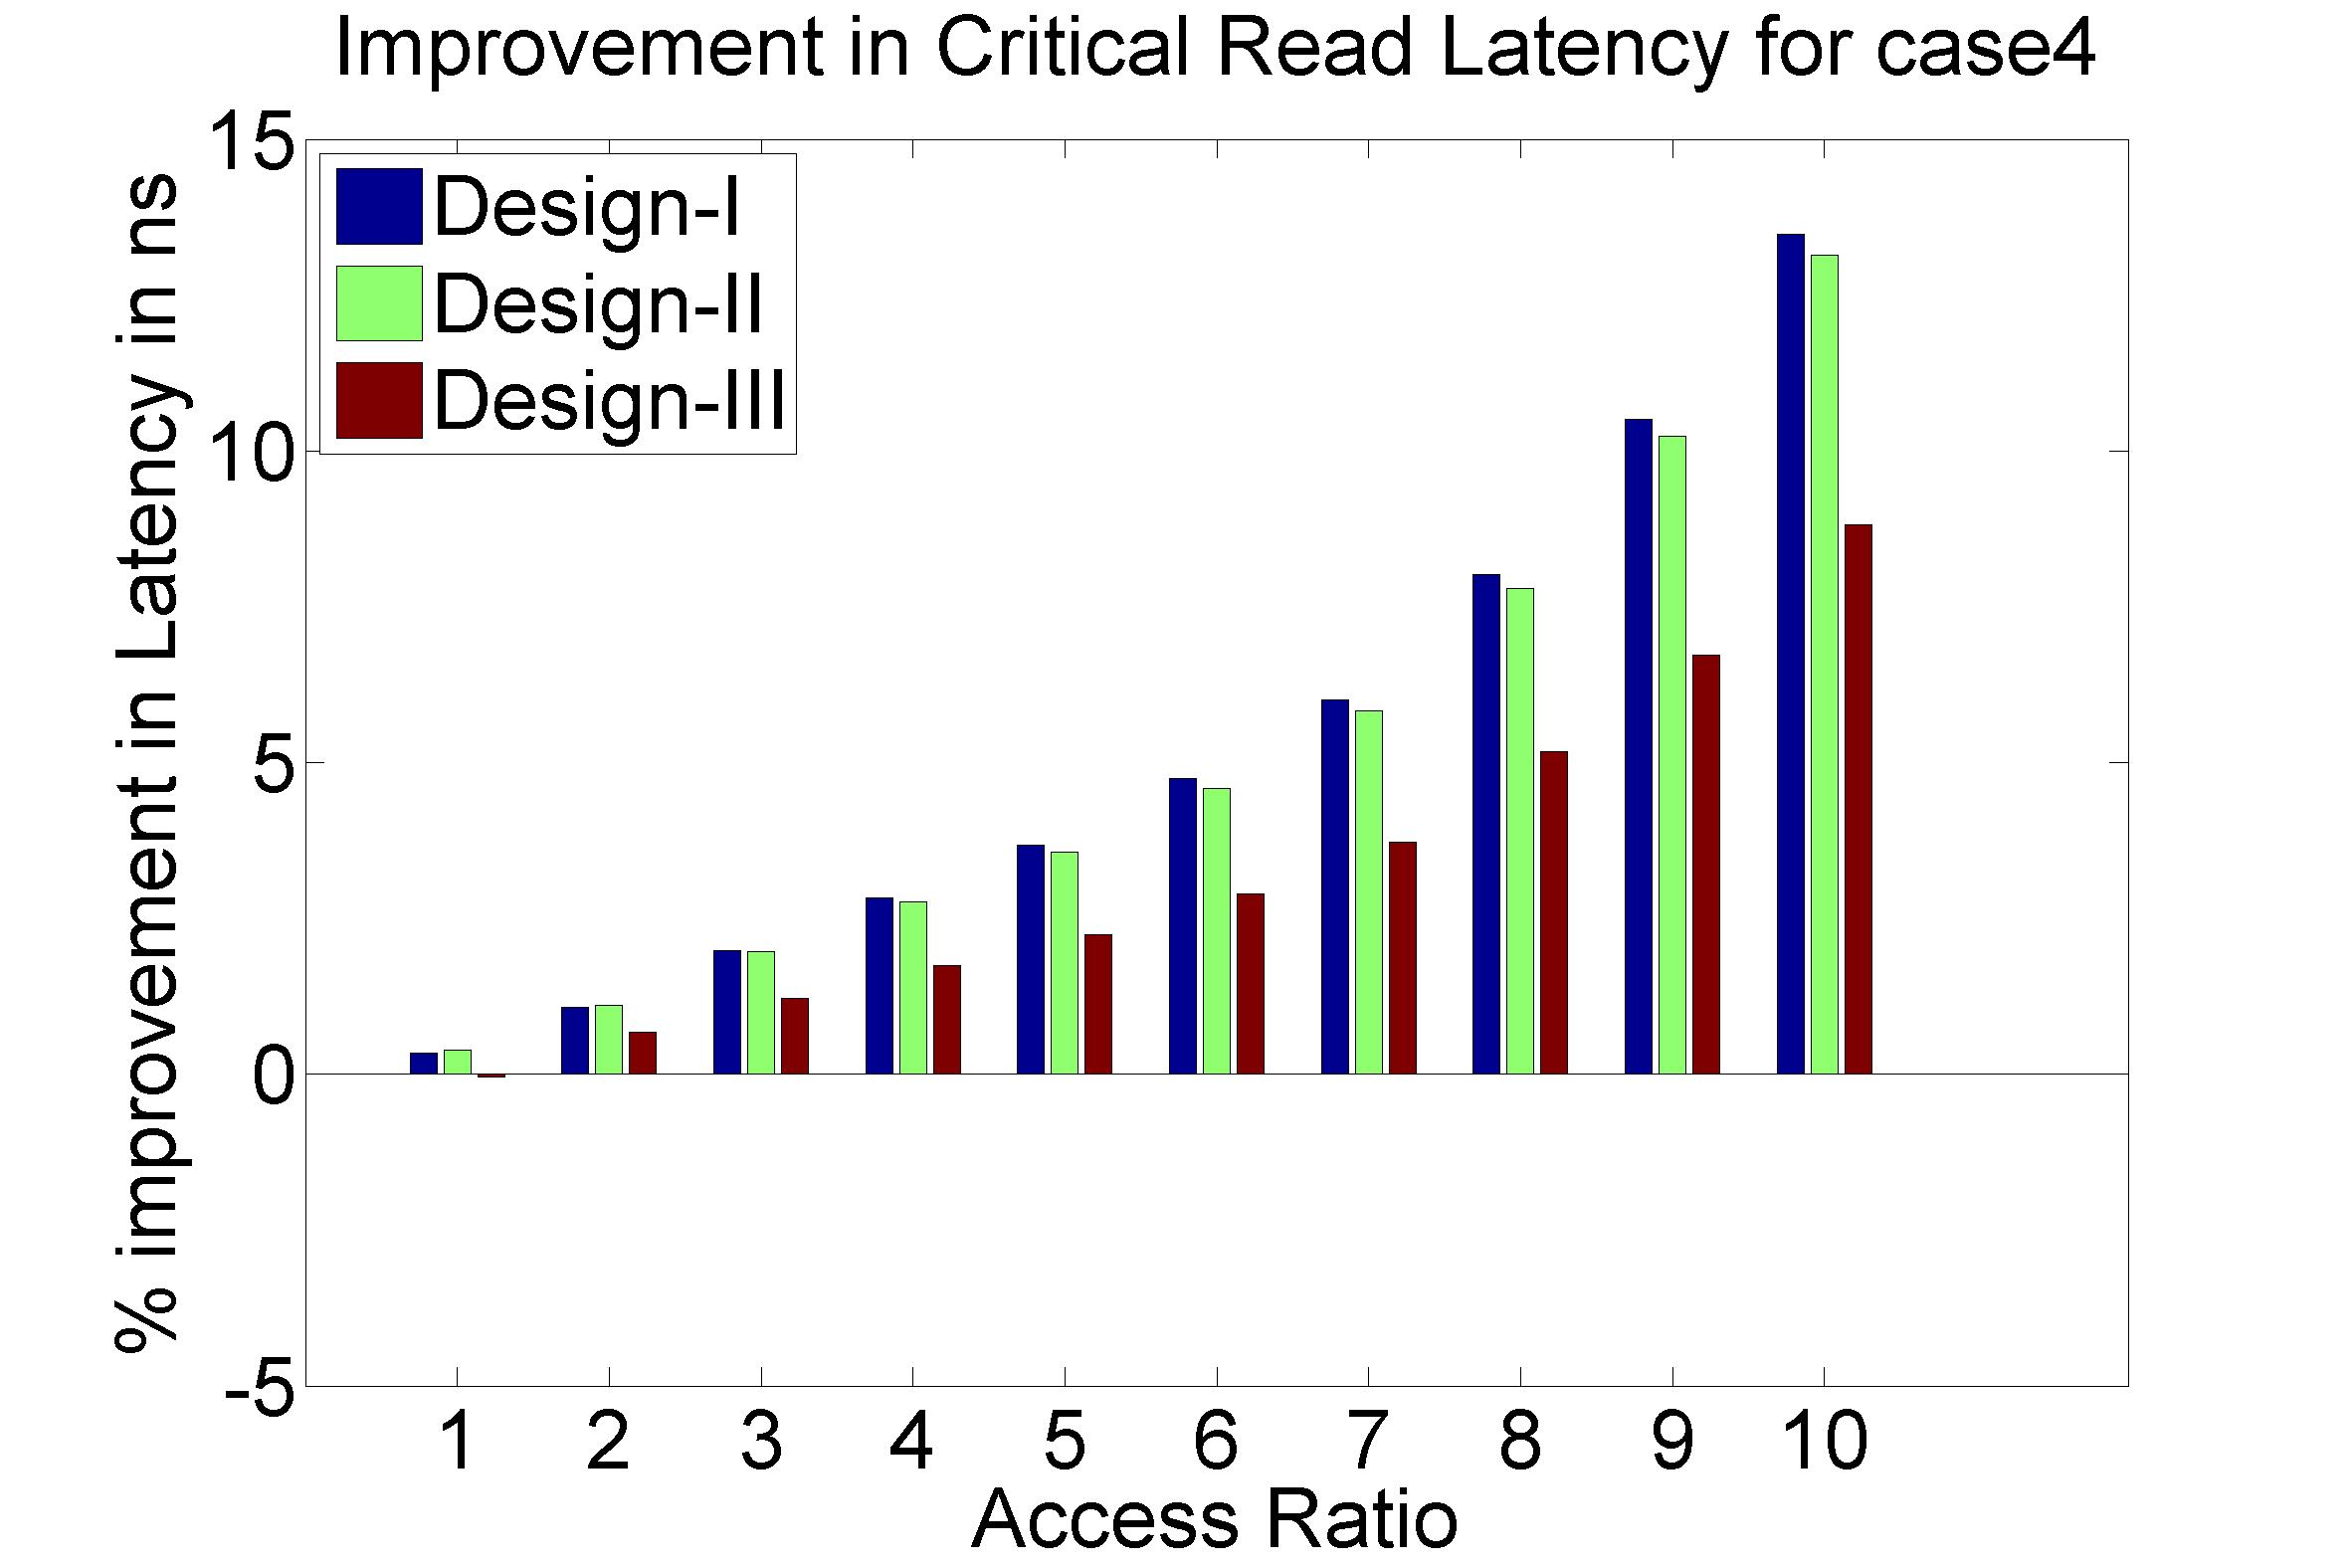
\includegraphics[width=\linewidth]{case4_critical_latency_improvement.jpeg}
\end{minipage}
\begin{minipage}[!t]{0.33\linewidth}
        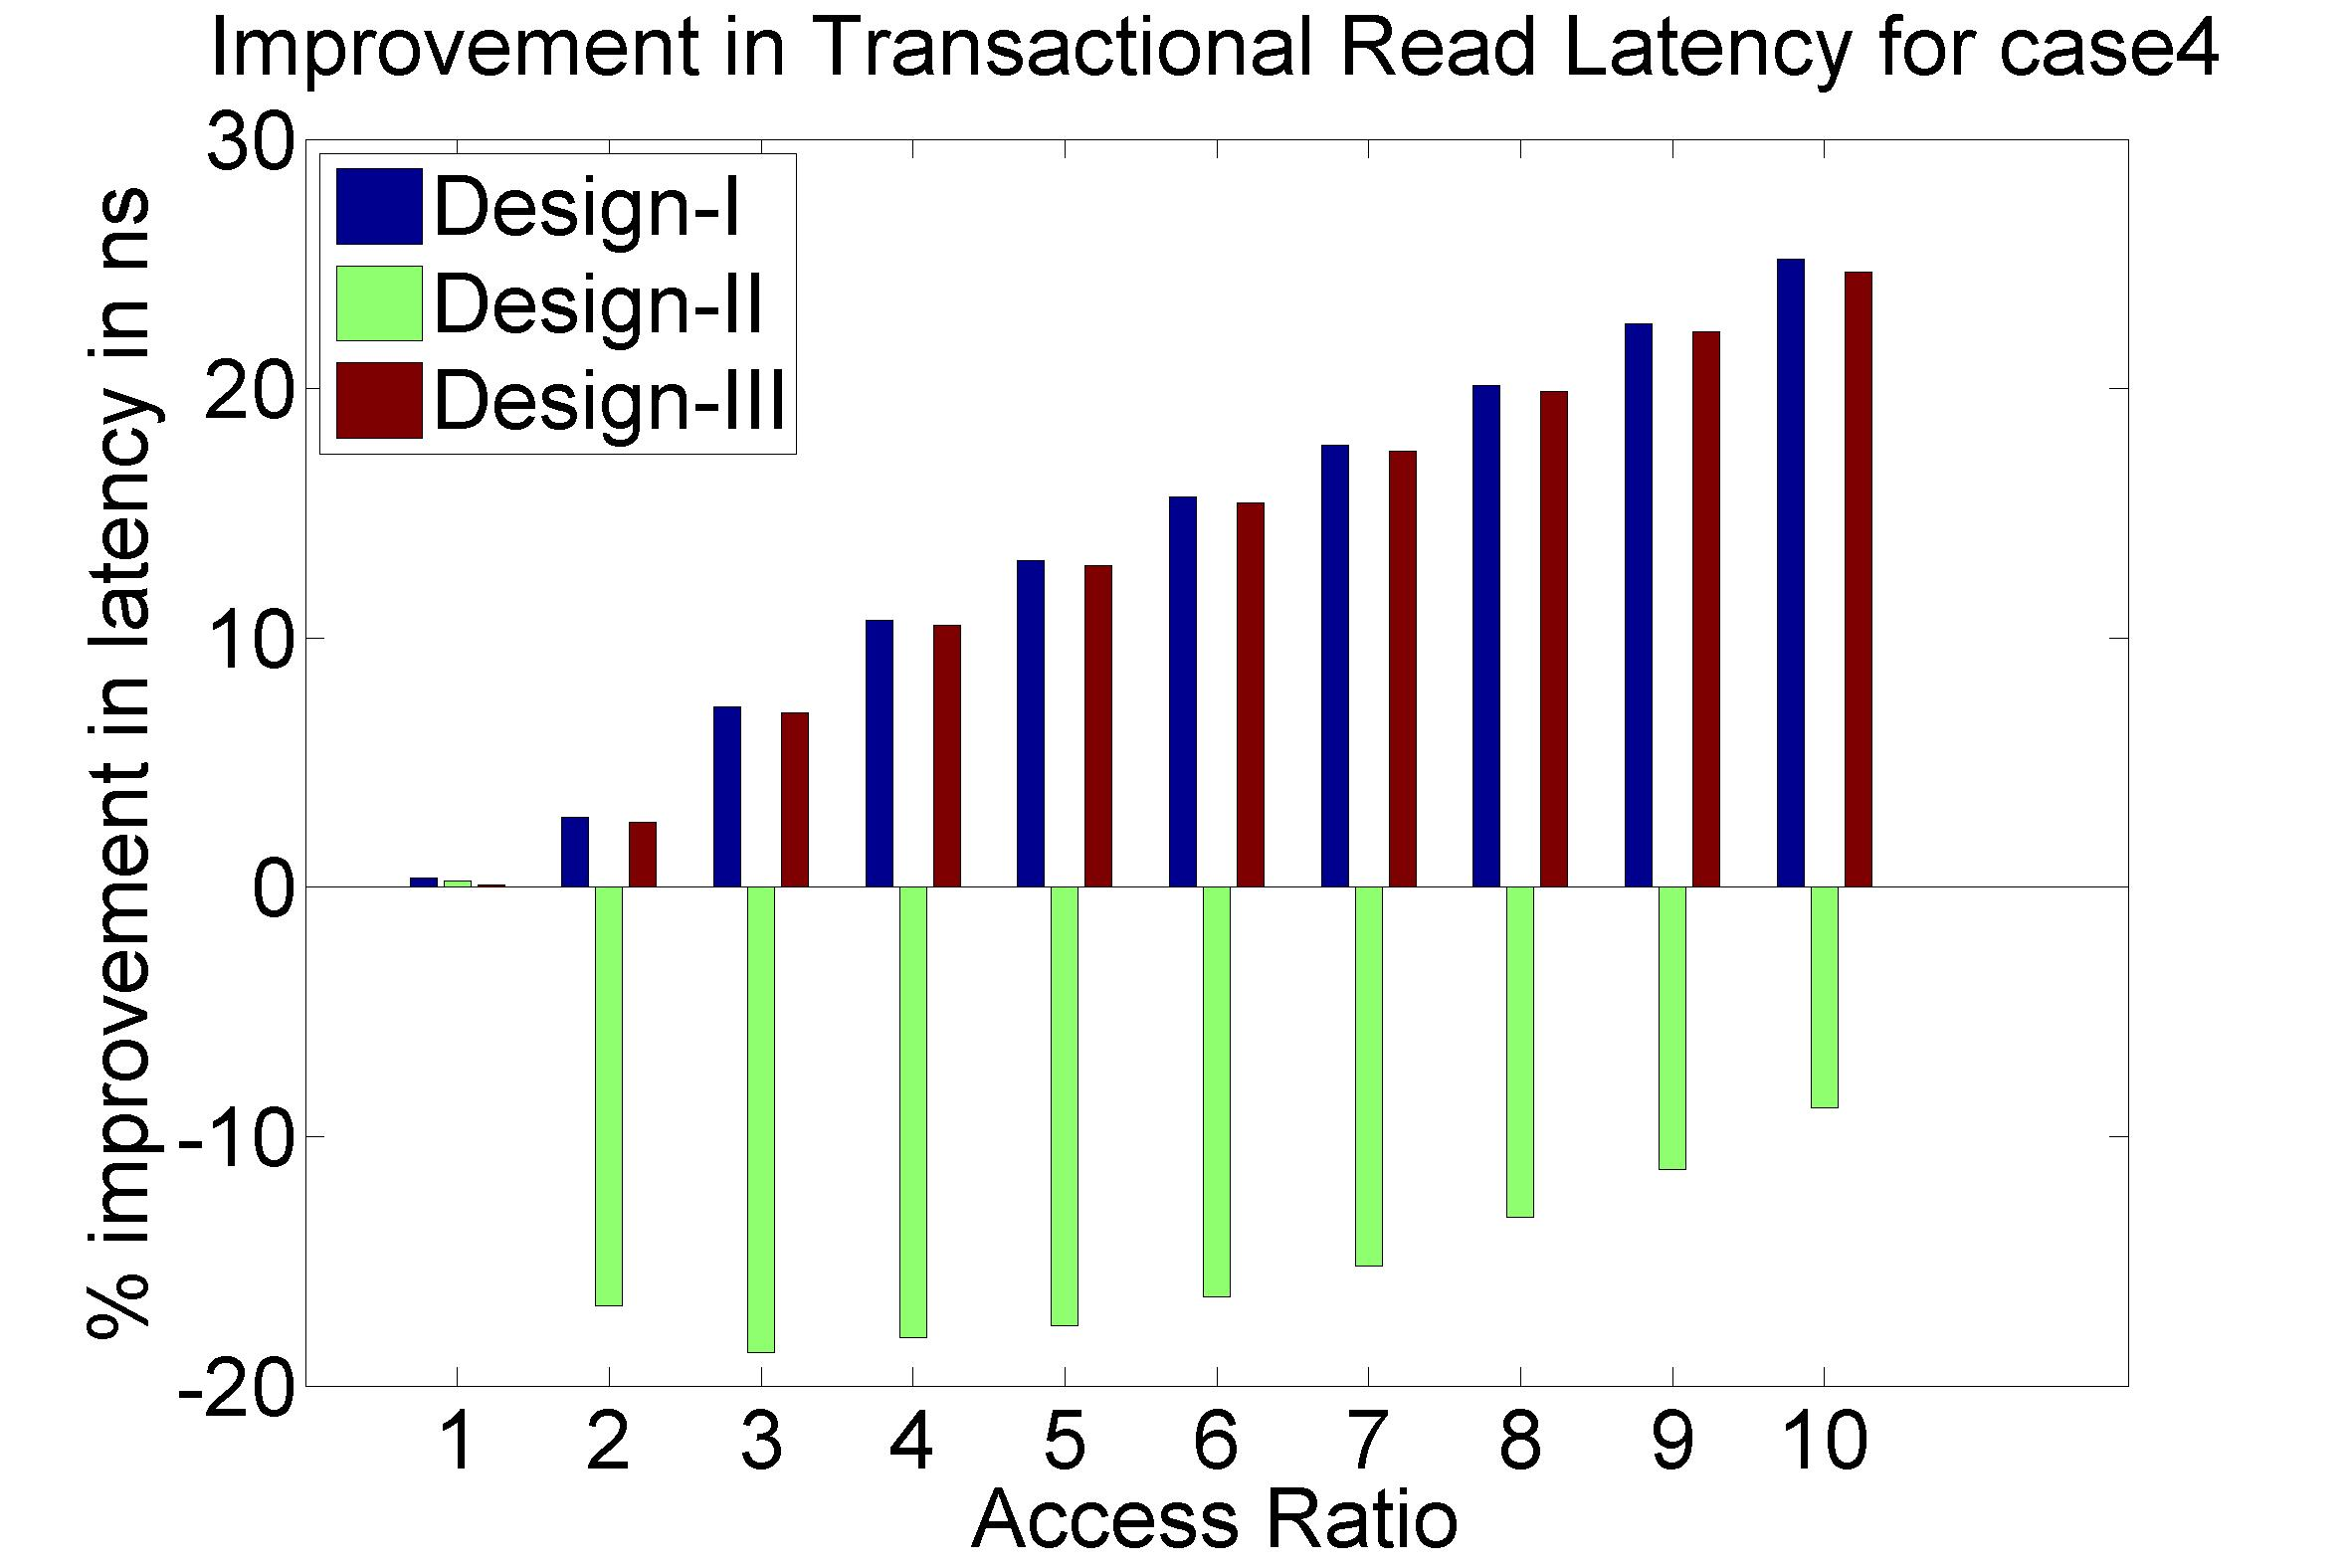
\includegraphics[width=\linewidth]{case4_transactional_latency_improvement.jpeg}
\end{minipage}
\begin{minipage}[!t]{0.33\linewidth}
        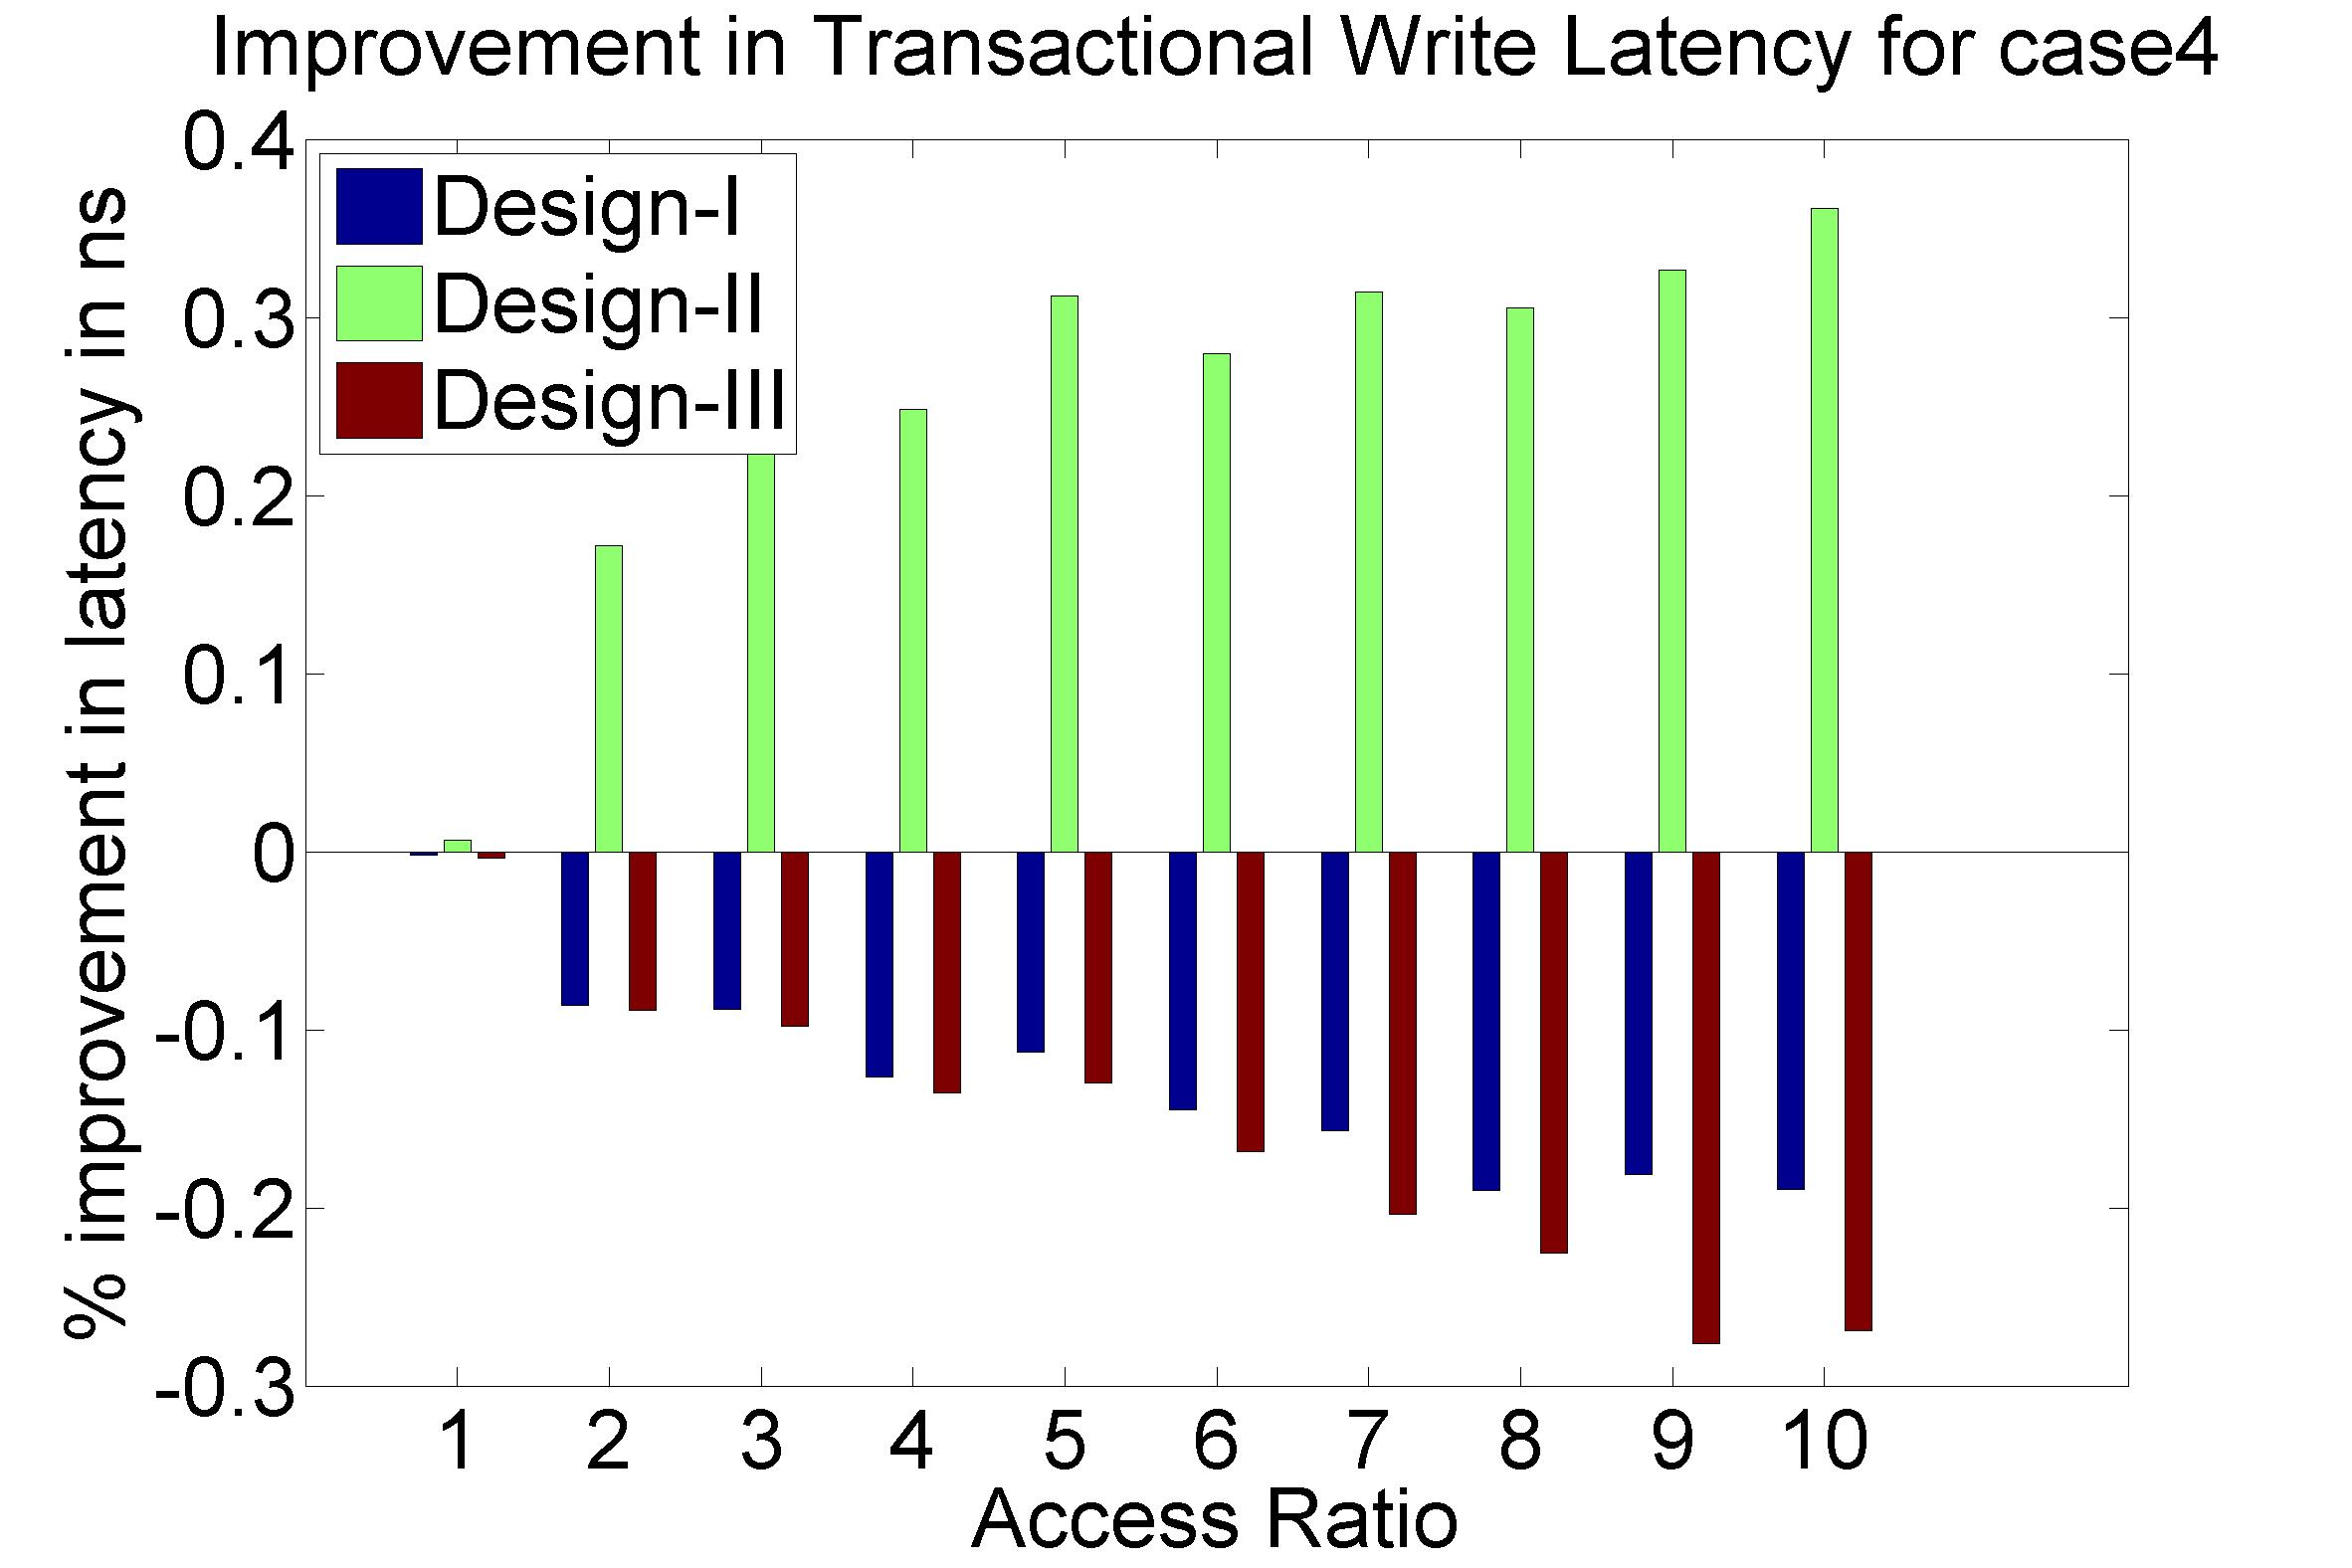
\includegraphics[width=\linewidth]{case4_write_latency_improvement.jpeg}
\end{minipage}
\caption{
{\bf Performance Graphs for case4 trace} }
\label{fig:case4_improvement}
\end{figure}
%-------------------------------------------------
Observations:
\begin{itemize}
	\item The case4 traces are low density traces. That is, the number of access requests per time period are low. 
	\item The Critical Read latency improvement in {\em positive} for all the ratios. 
	\item The critical read latency exponentially improves for increased access ratios.
	\item The transactional Read latency also improves for design I and design III. 
	\item The write latency has only marginal improvement. 
	\item The results suggest that in case4, we do not use the "coding" aspect due to low density access in case of Writes.
	\item The improvement in Transactional Read Latency is substantial. 
\end{itemize}
\cleardoublepage
%-------------------------------------------------
\begin{figure}[htb]
\begin{minipage}[!t]{\linewidth}
        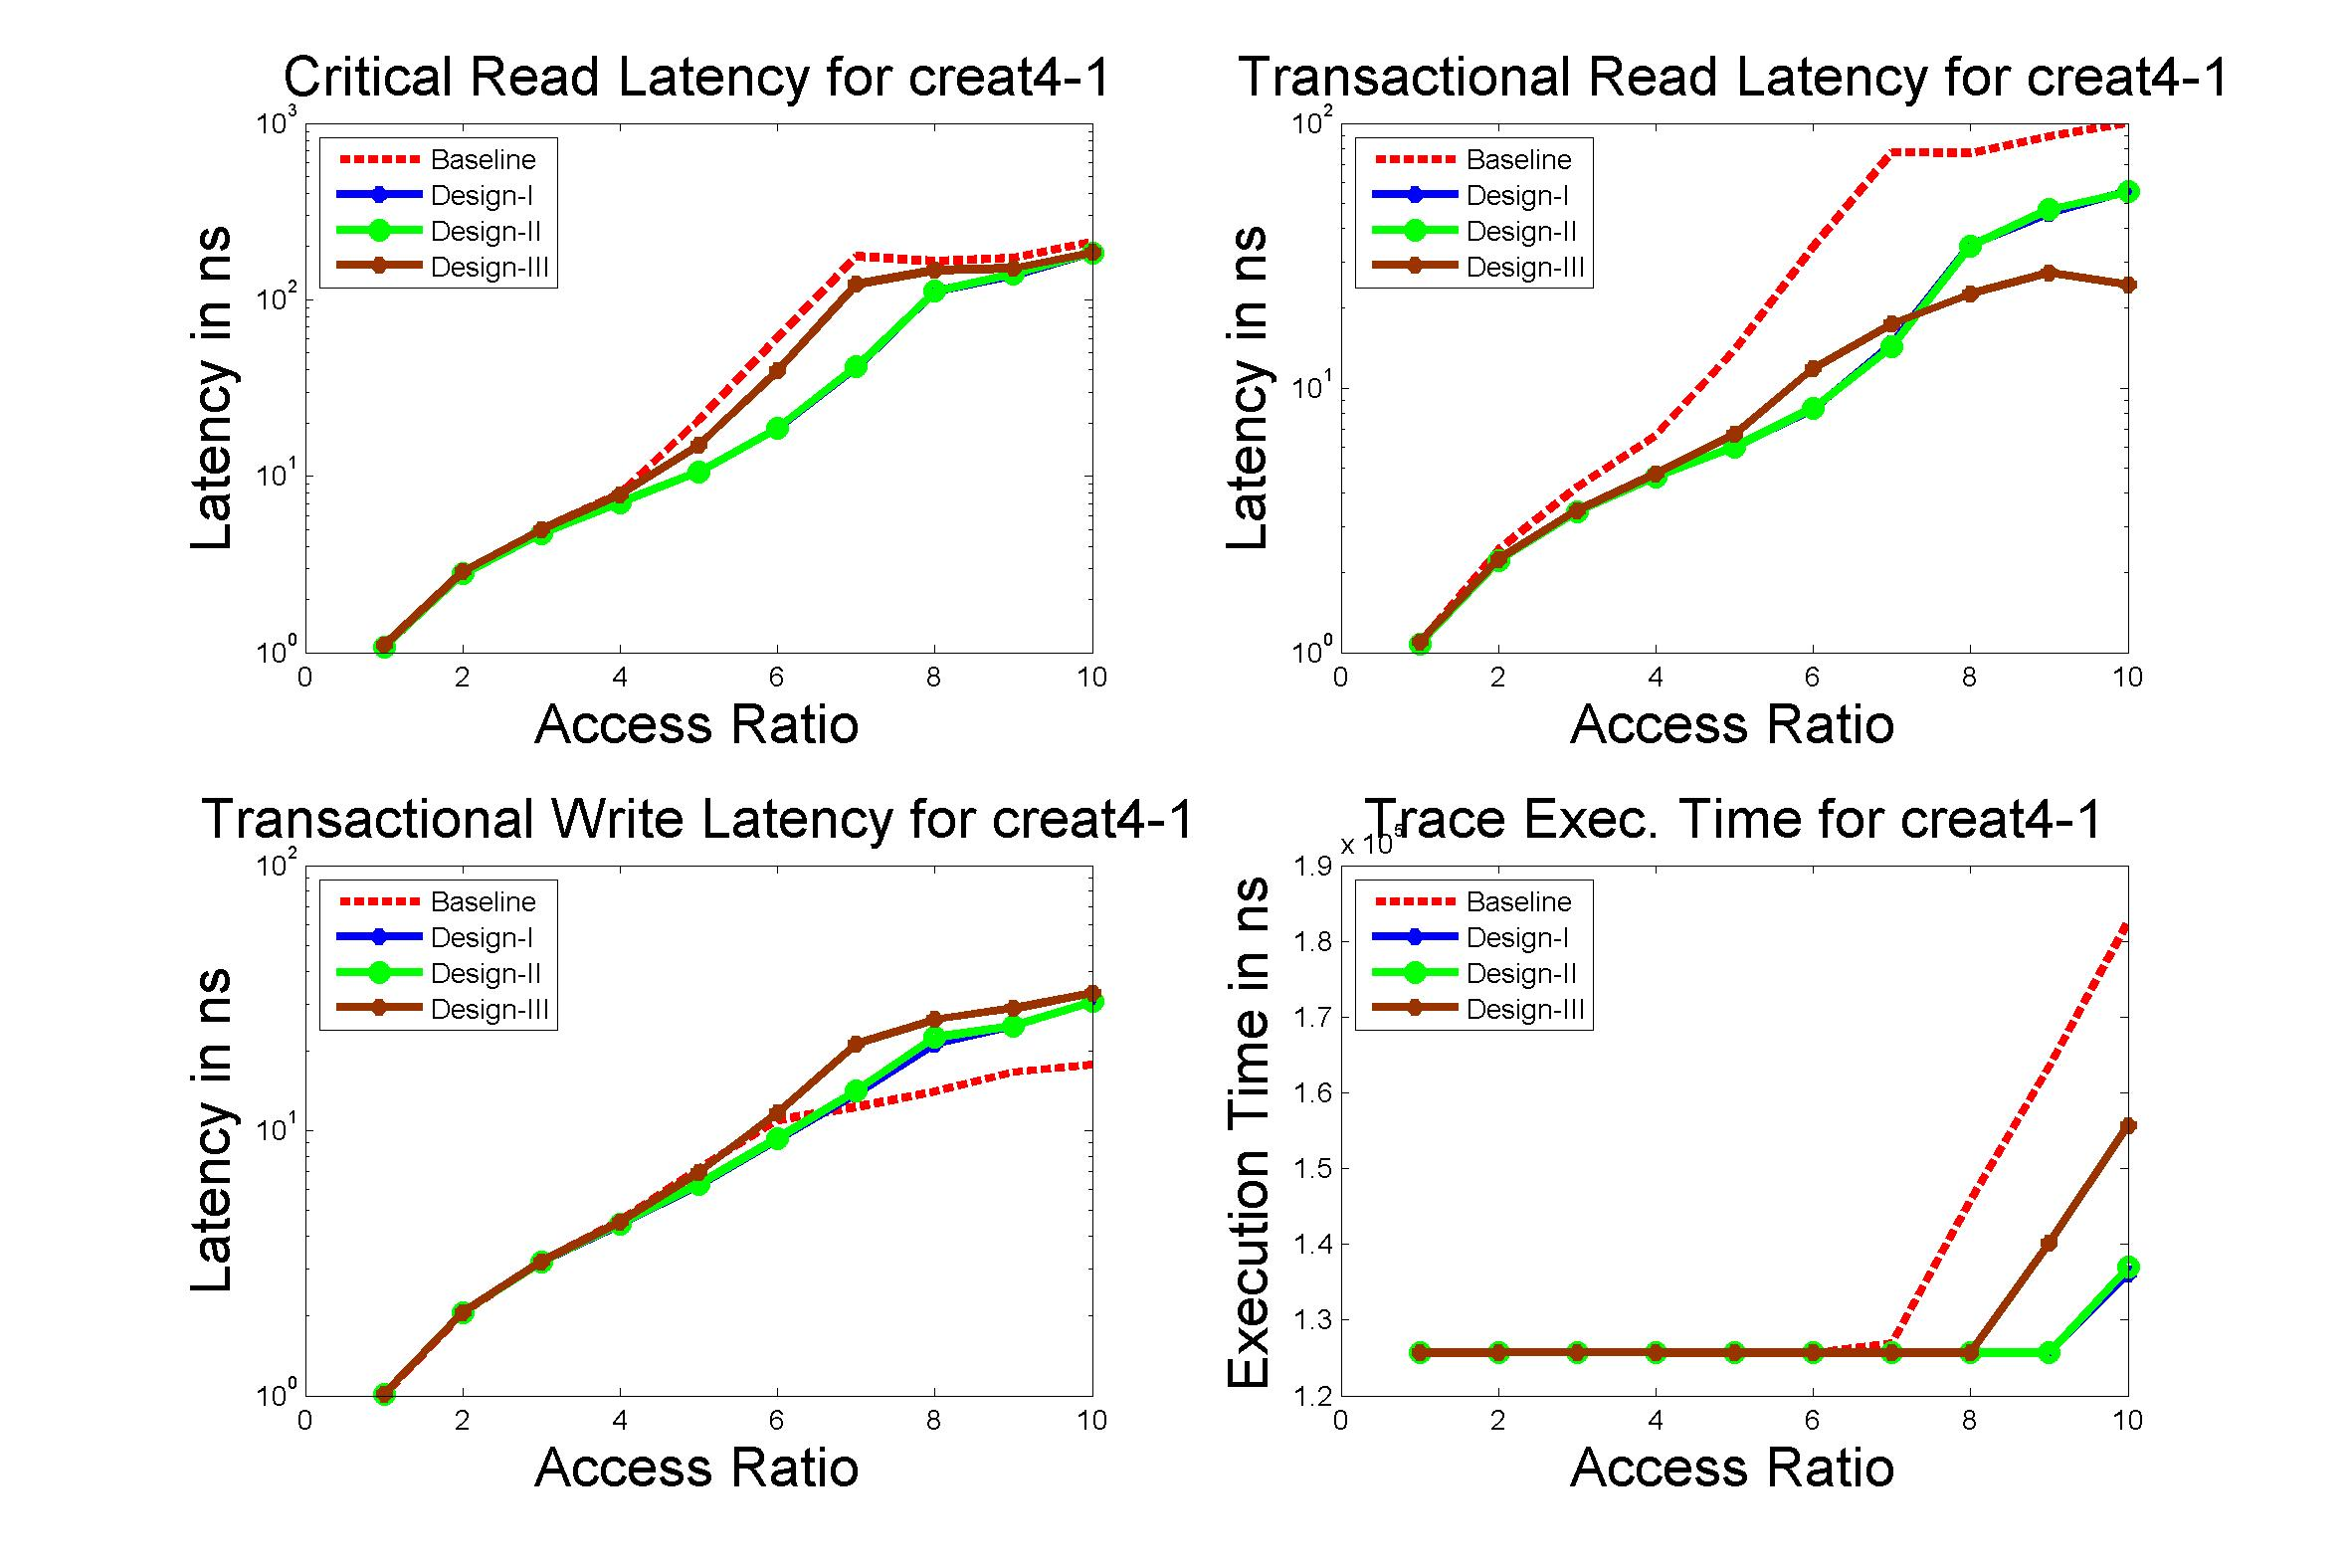
\includegraphics[width=\linewidth]{creat4-1.jpg}
\end{minipage}
\caption{
{\bf Performance Graphs for Creat4-1 trace} }
\label{fig:creat41}
\end{figure}
%-------------------------------------------------
\cleardoublepage
%-------------------------------------------------
\begin{figure}[htb]
\begin{minipage}[!t]{0.33\linewidth}
        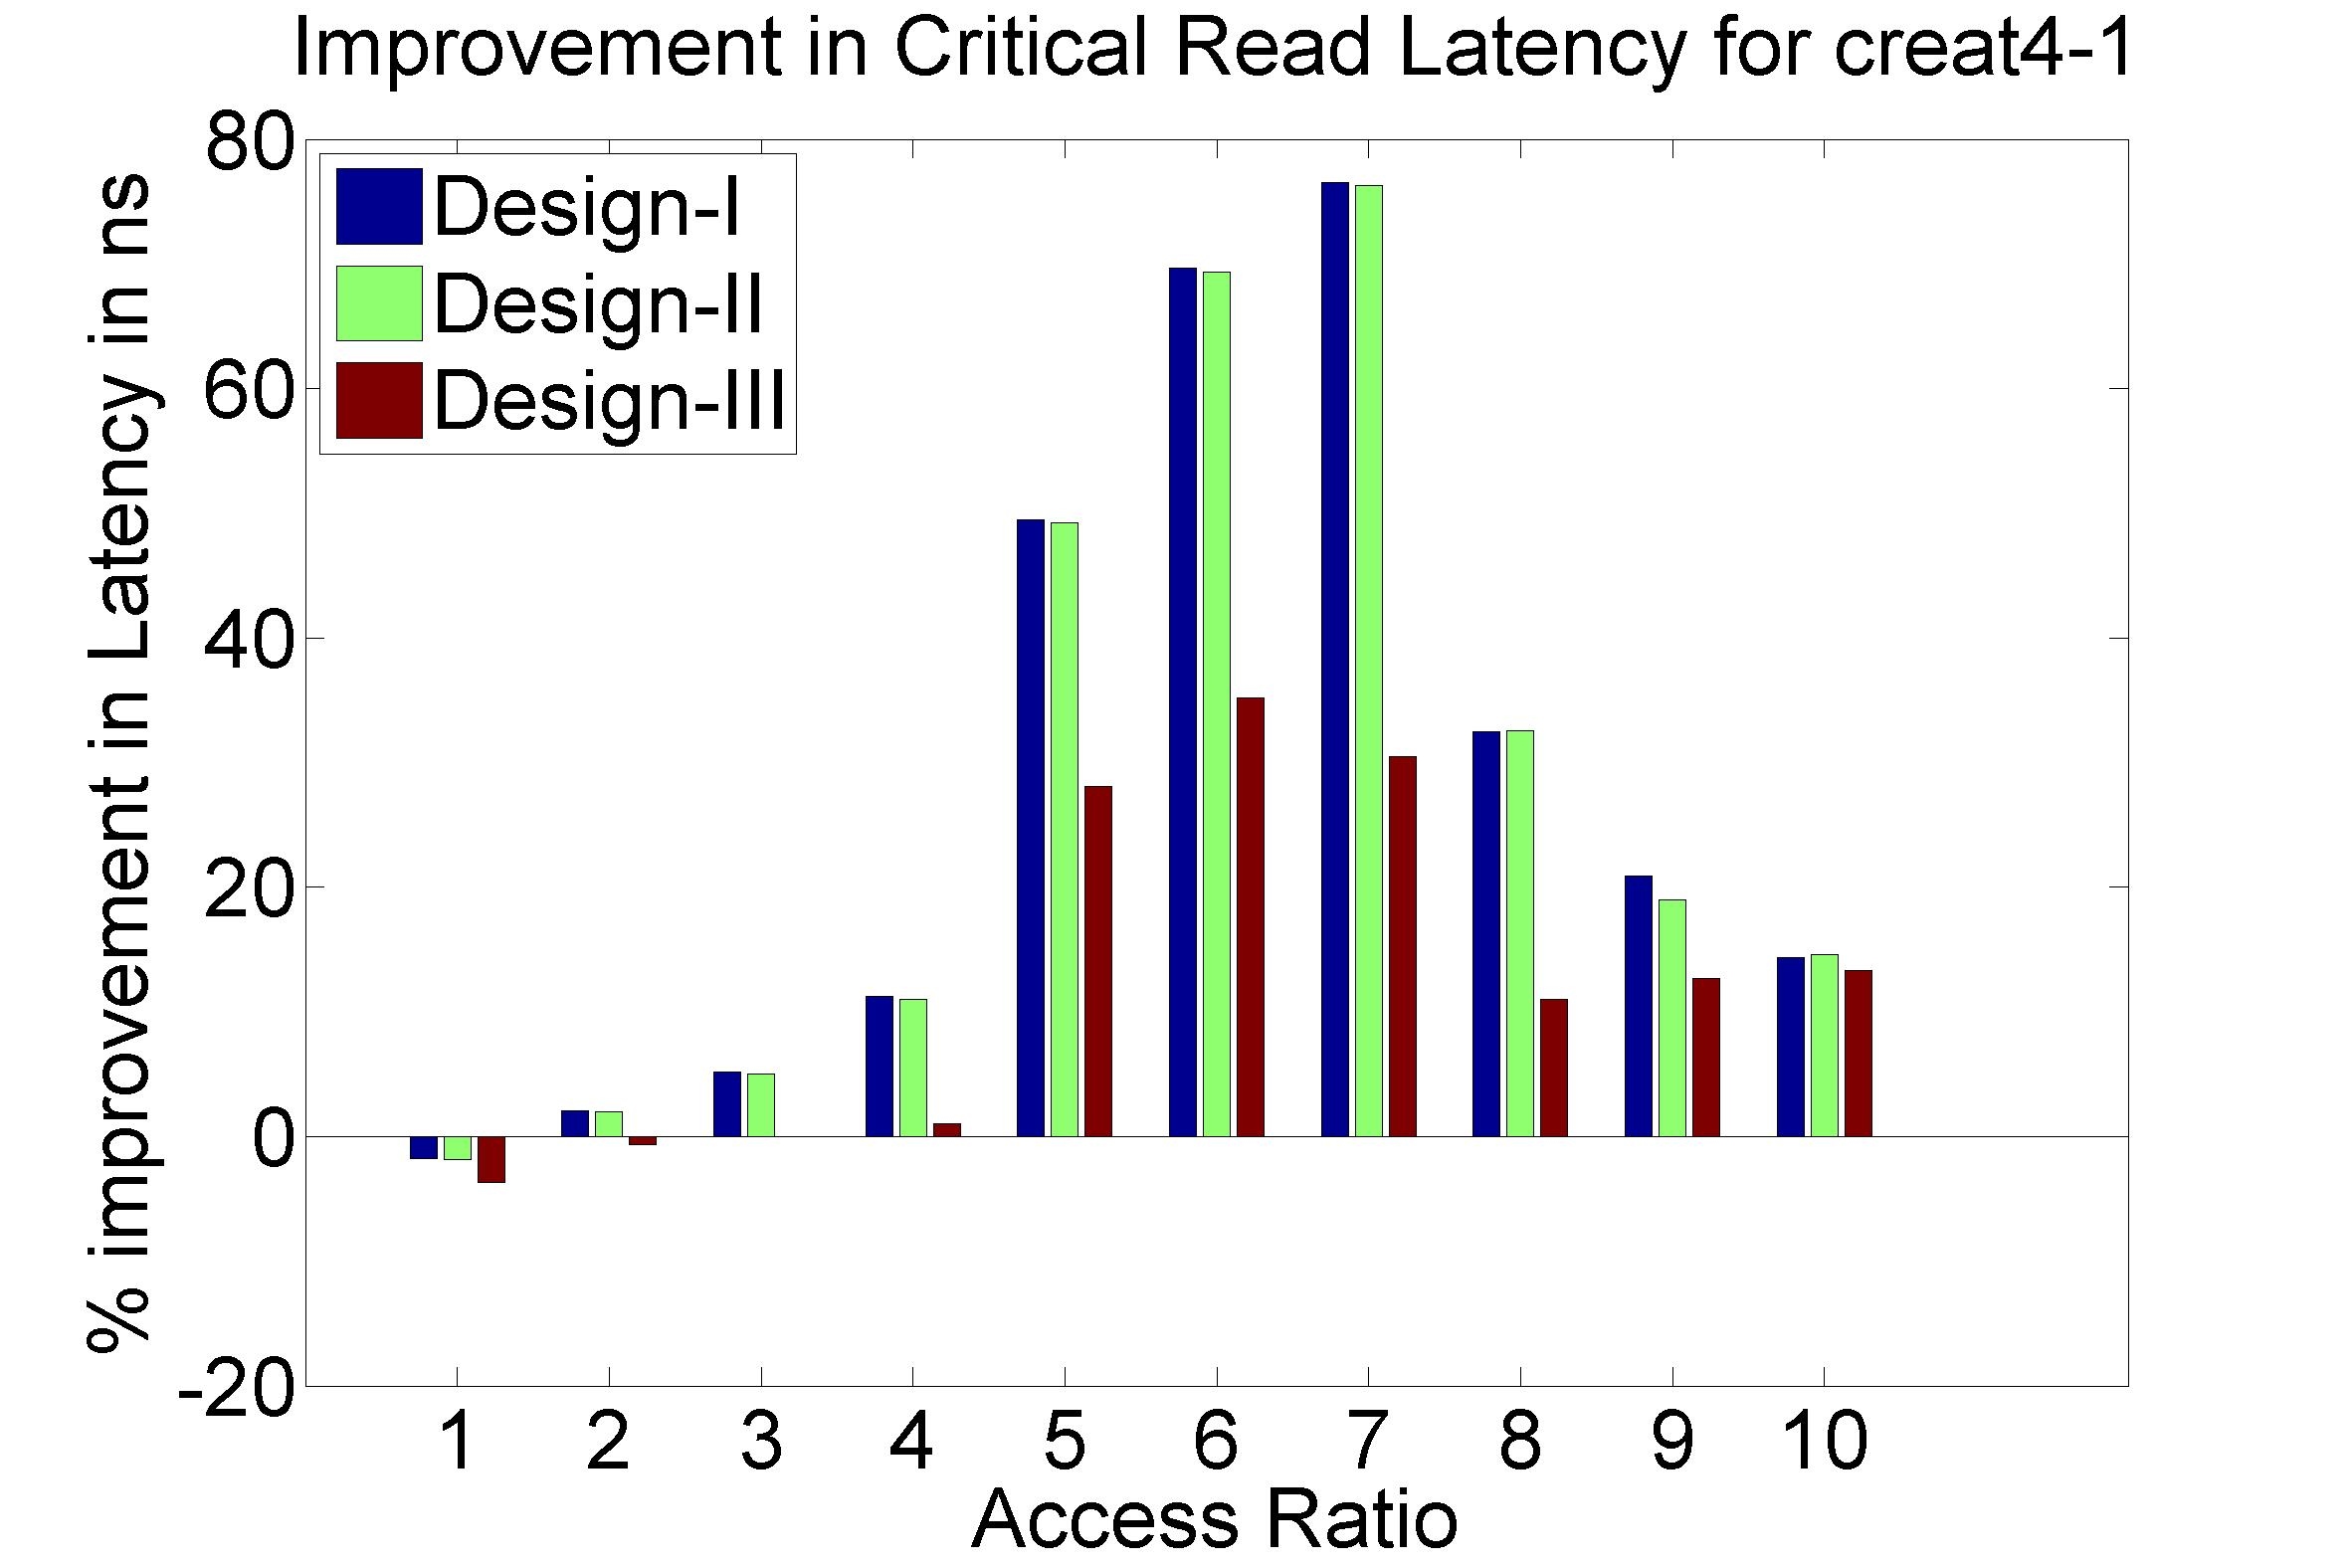
\includegraphics[width=\linewidth]{creat4-1_critical_latency_improvement.jpeg}
\end{minipage}
\begin{minipage}[!t]{0.33\linewidth}
        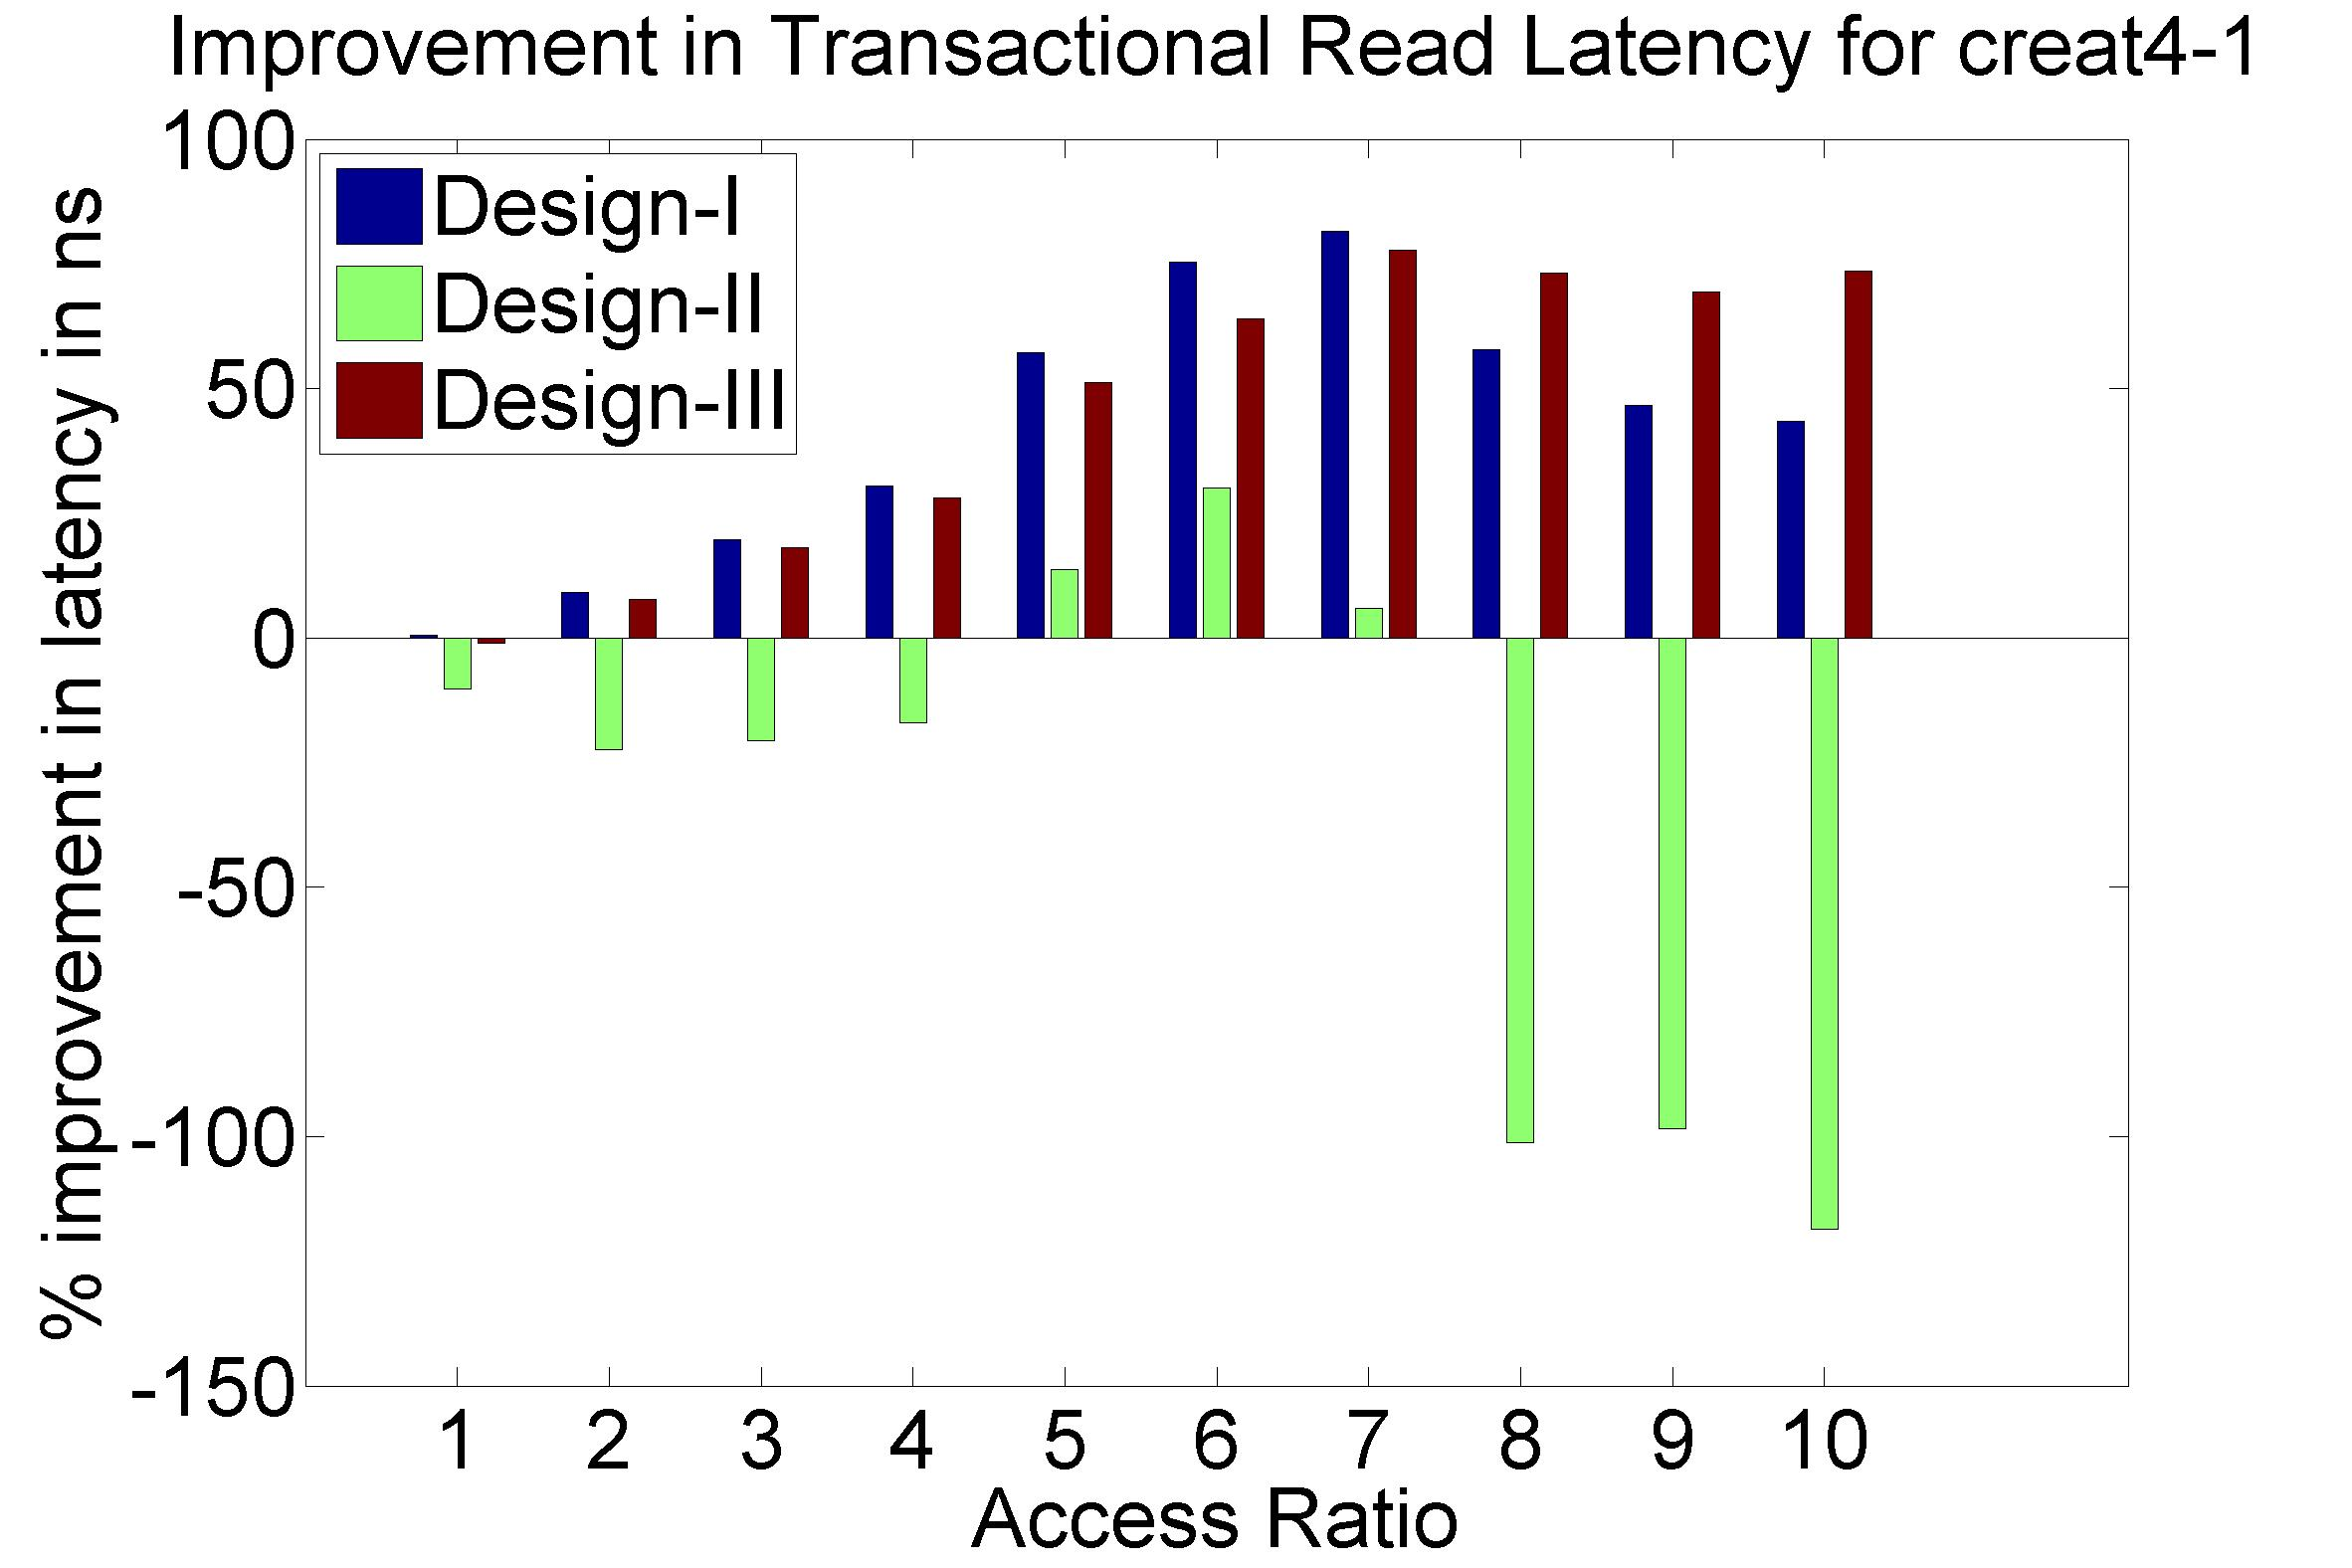
\includegraphics[width=\linewidth]{creat4-1_transactional_latency_improvement.jpeg}
\end{minipage}
\begin{minipage}[!t]{0.33\linewidth}
        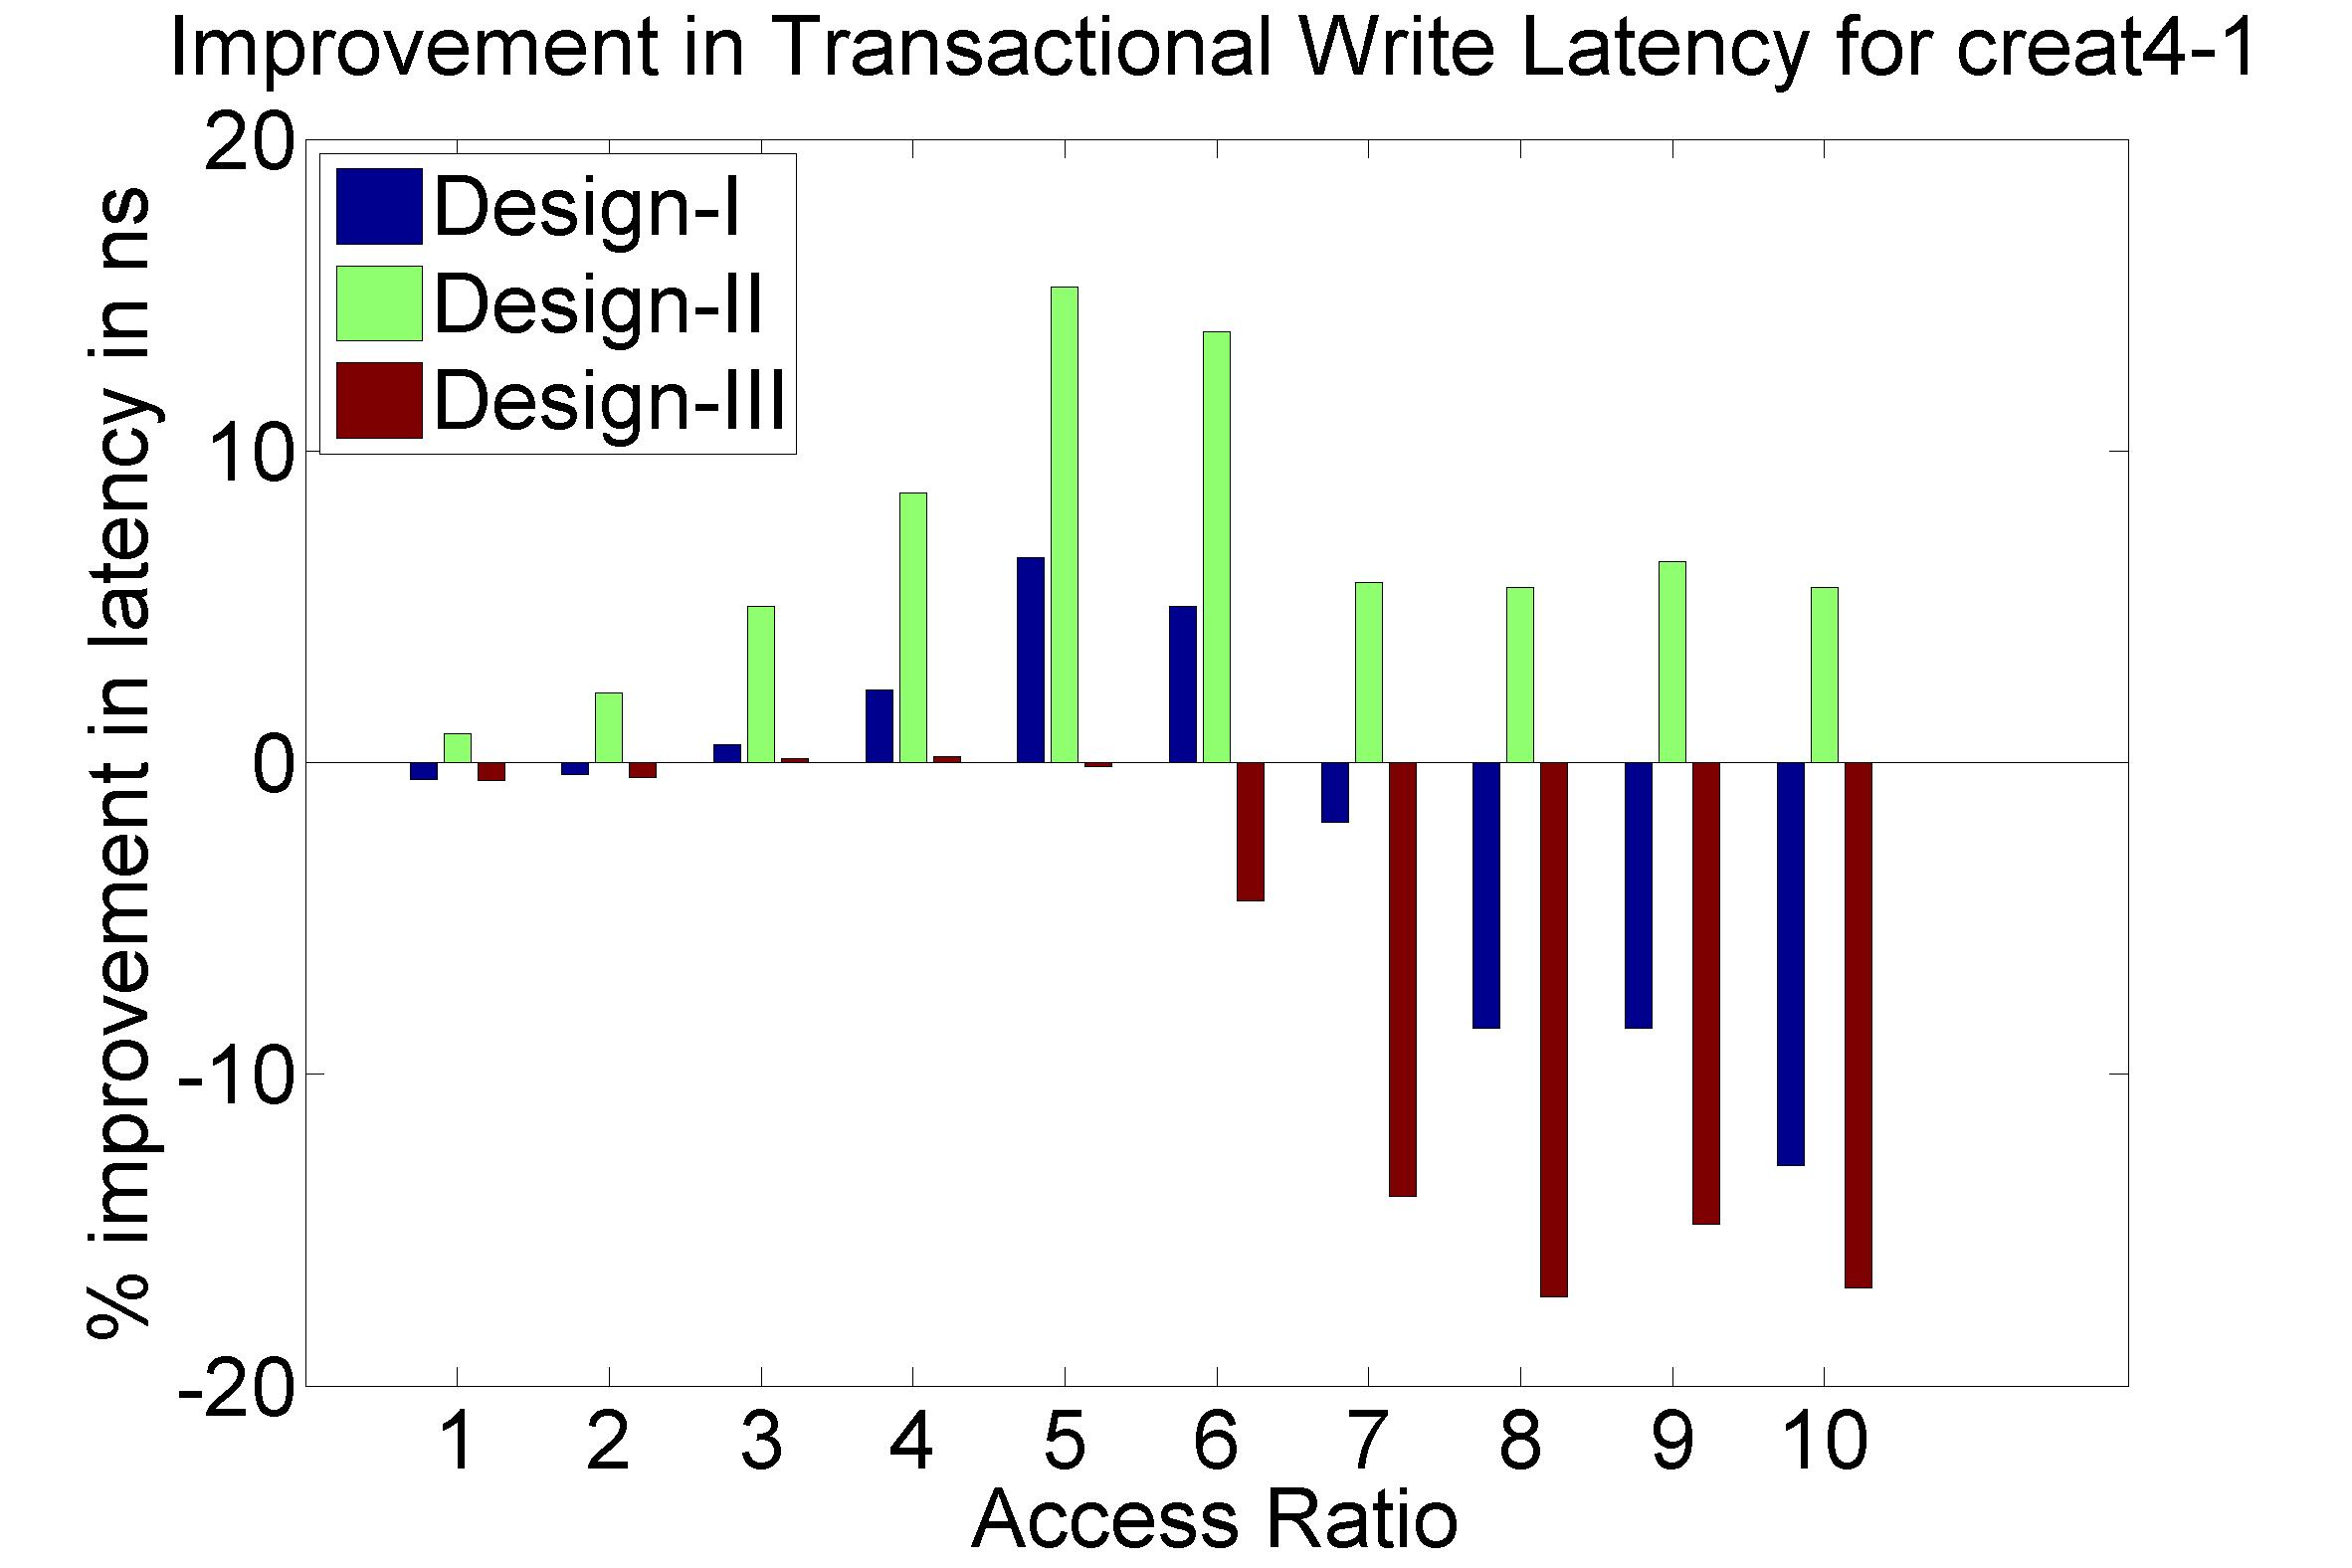
\includegraphics[width=\linewidth]{creat4-1_write_latency_improvement.jpeg}
\end{minipage}
\caption{
{\bf Performance Graphs for Creat4-1 trace} }
\label{fig:creat41_improvement}
\end{figure}
%-------------------------------------------------
Observations:
\begin{itemize}
	\item The trace creat4-1 is a medium density trace. 
	\item The improvement in critical read latency and transactional read latency is significant in design I and design II. 
	\item The write latency is positive till access ratio of 6.
	\item Design I and Design III codes benefit in this trace.
\end{itemize}
\cleardoublepage
%-------------------------------------------------
\begin{figure}[htb]
\begin{minipage}[!t]{\linewidth}
        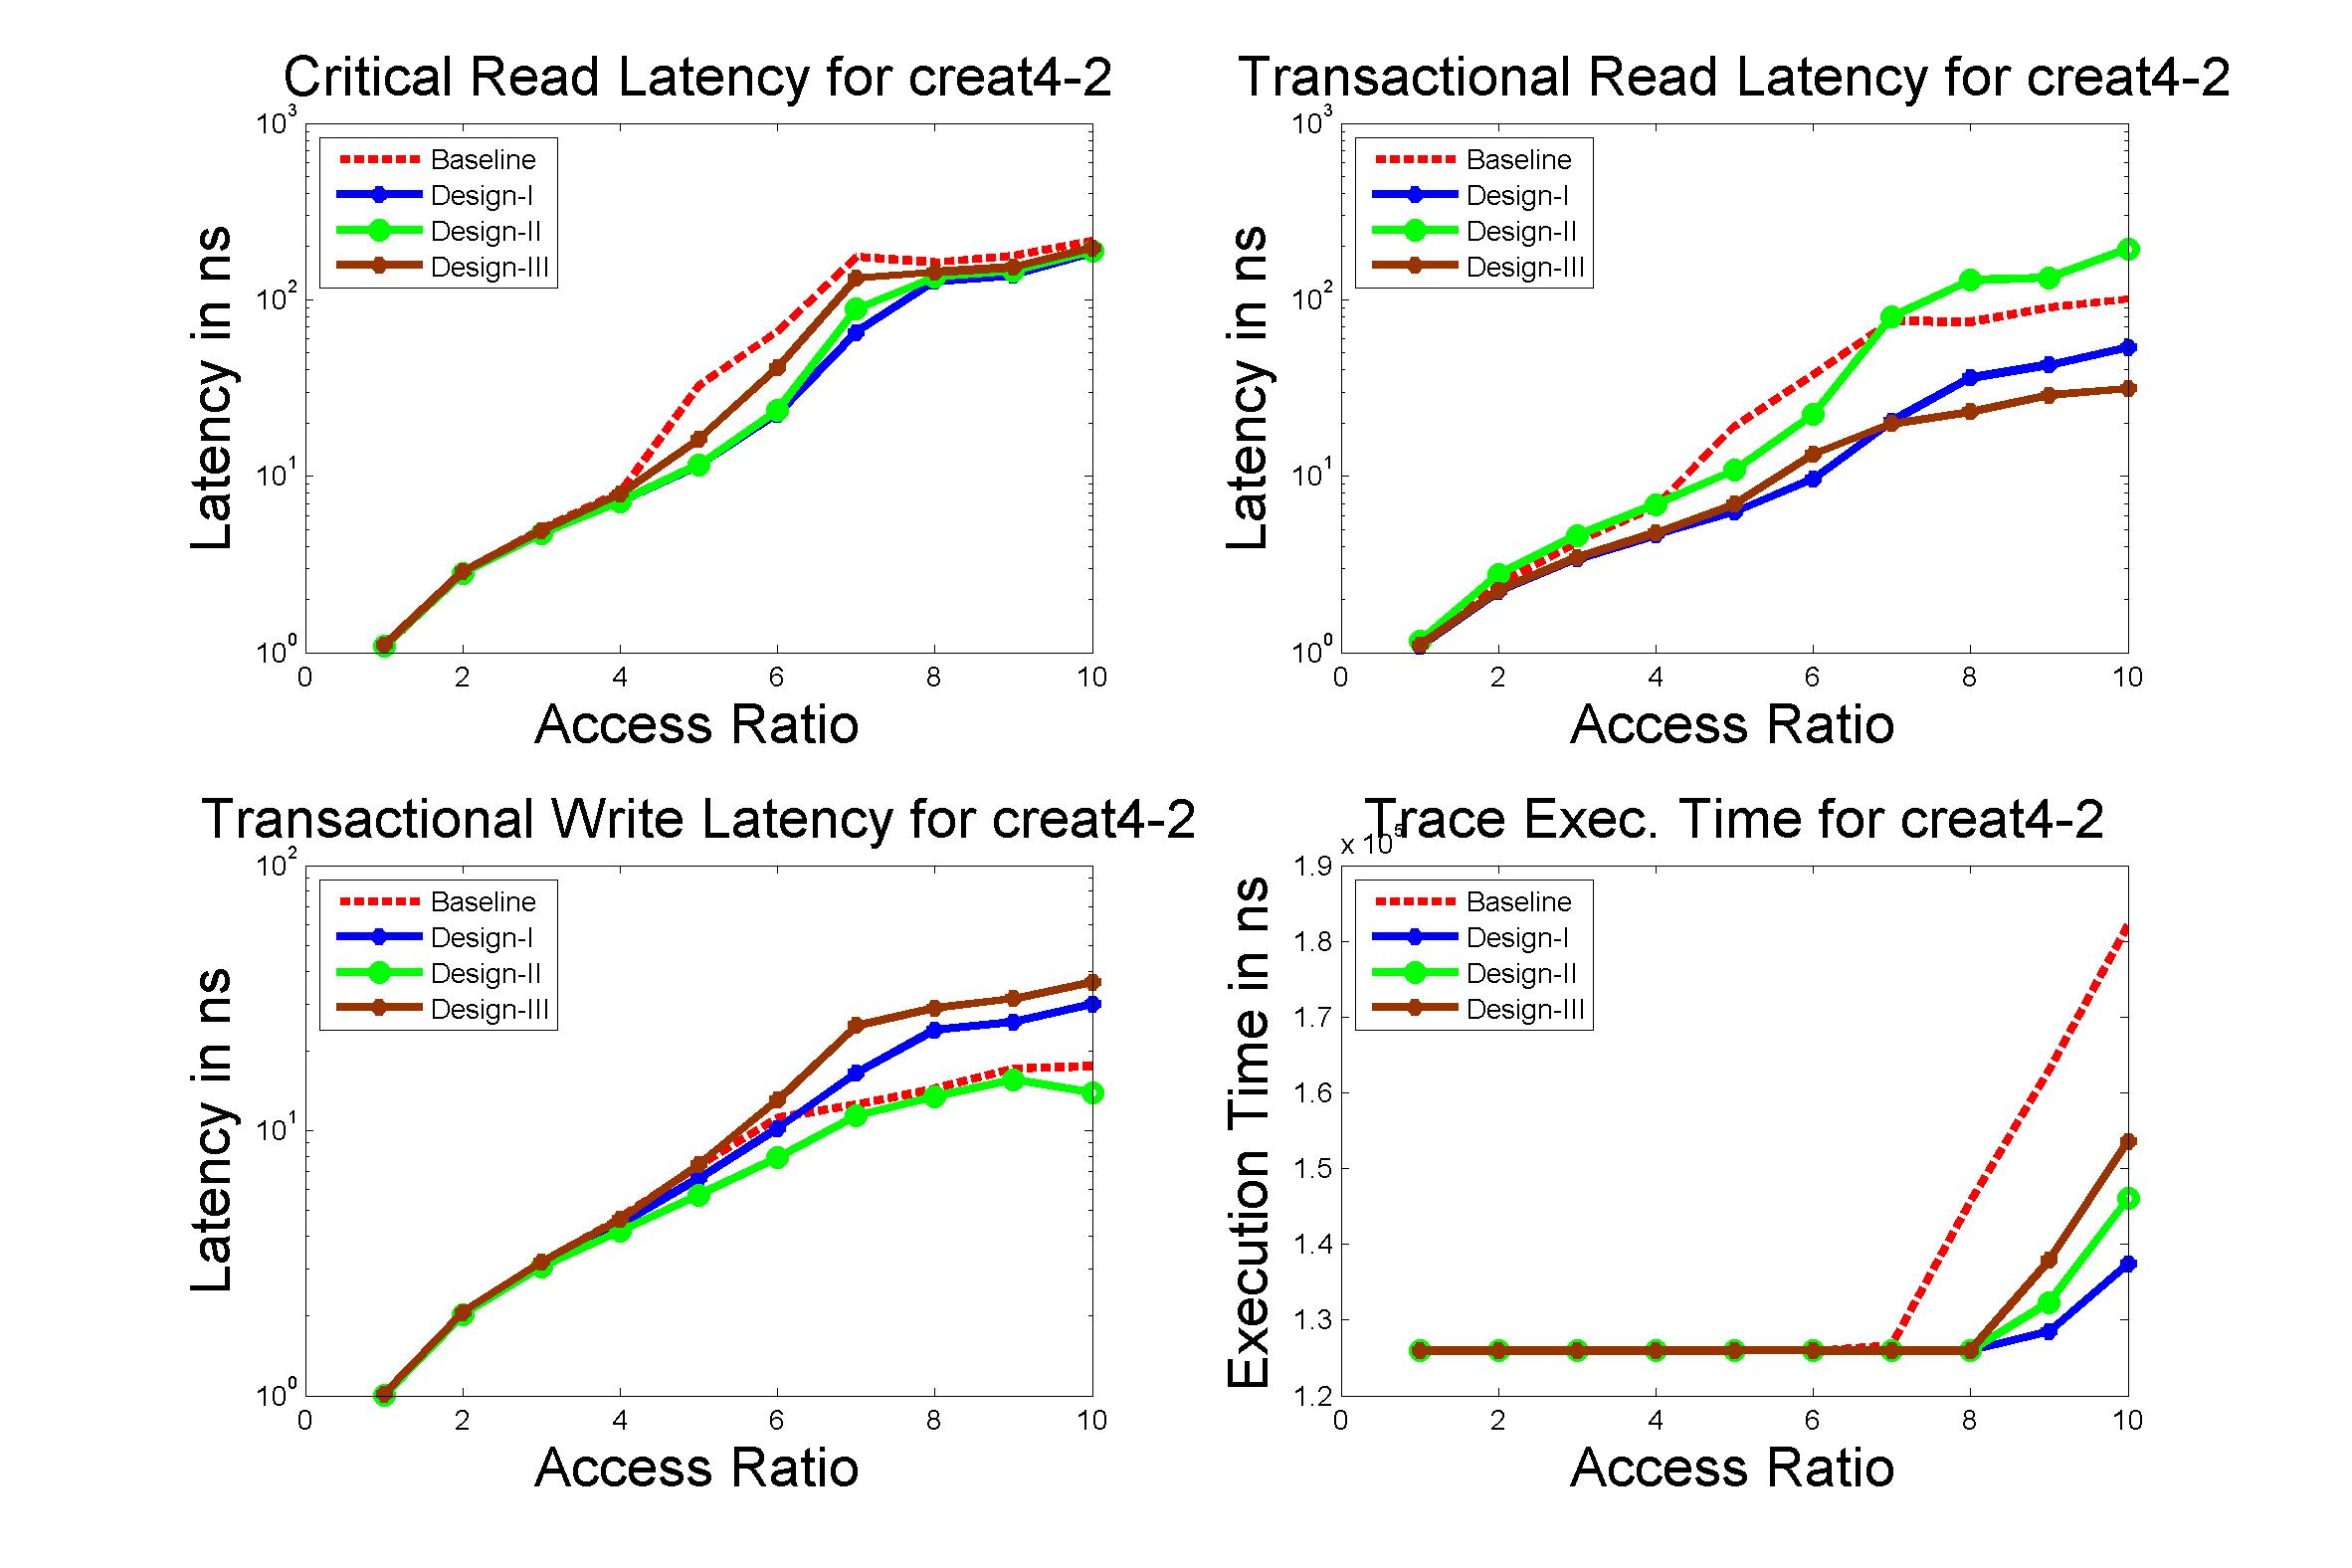
\includegraphics[width=\linewidth]{creat4-2.jpg}
\end{minipage}
\caption{
{\bf Performance Graphs for Creat4-2 trace} }
\label{fig:creat42}
\end{figure}
%-------------------------------------------------
\cleardoublepage
%-------------------------------------------------
\begin{figure}[htb]
\begin{minipage}[!t]{0.33\linewidth}
        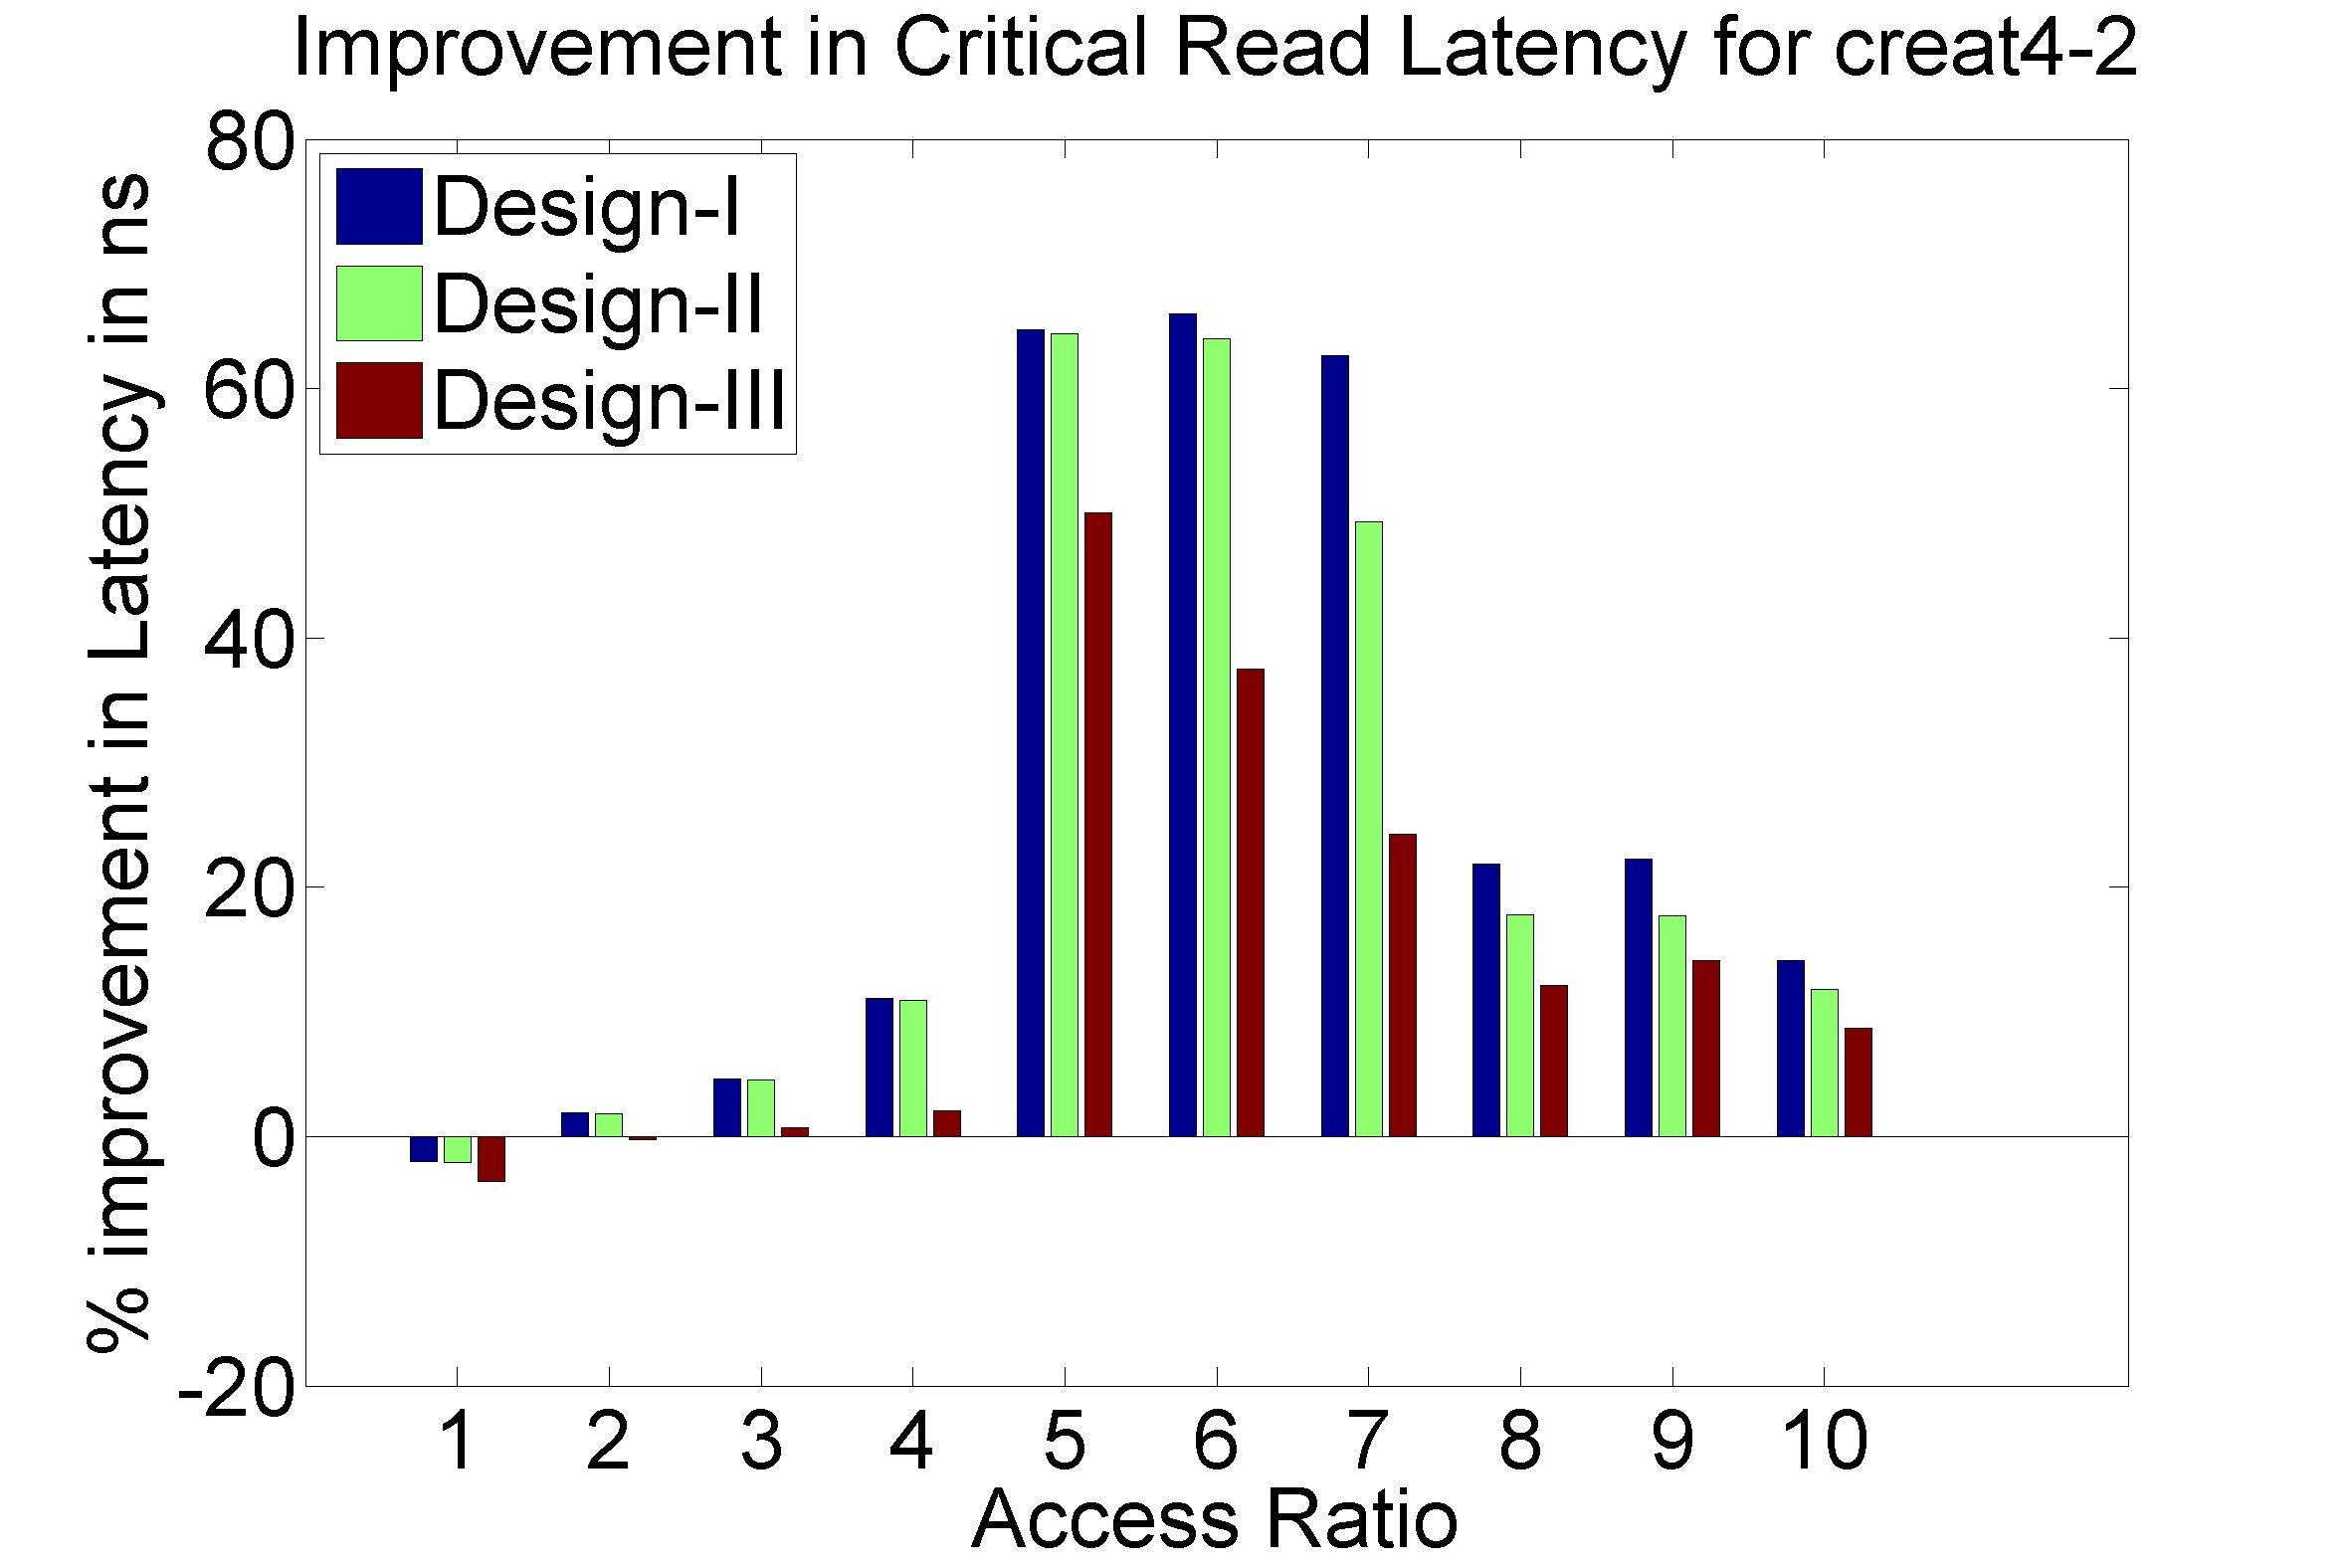
\includegraphics[width=\linewidth]{creat4-2_critical_latency_improvement.jpeg}
\end{minipage}
\begin{minipage}[!t]{0.33\linewidth}
        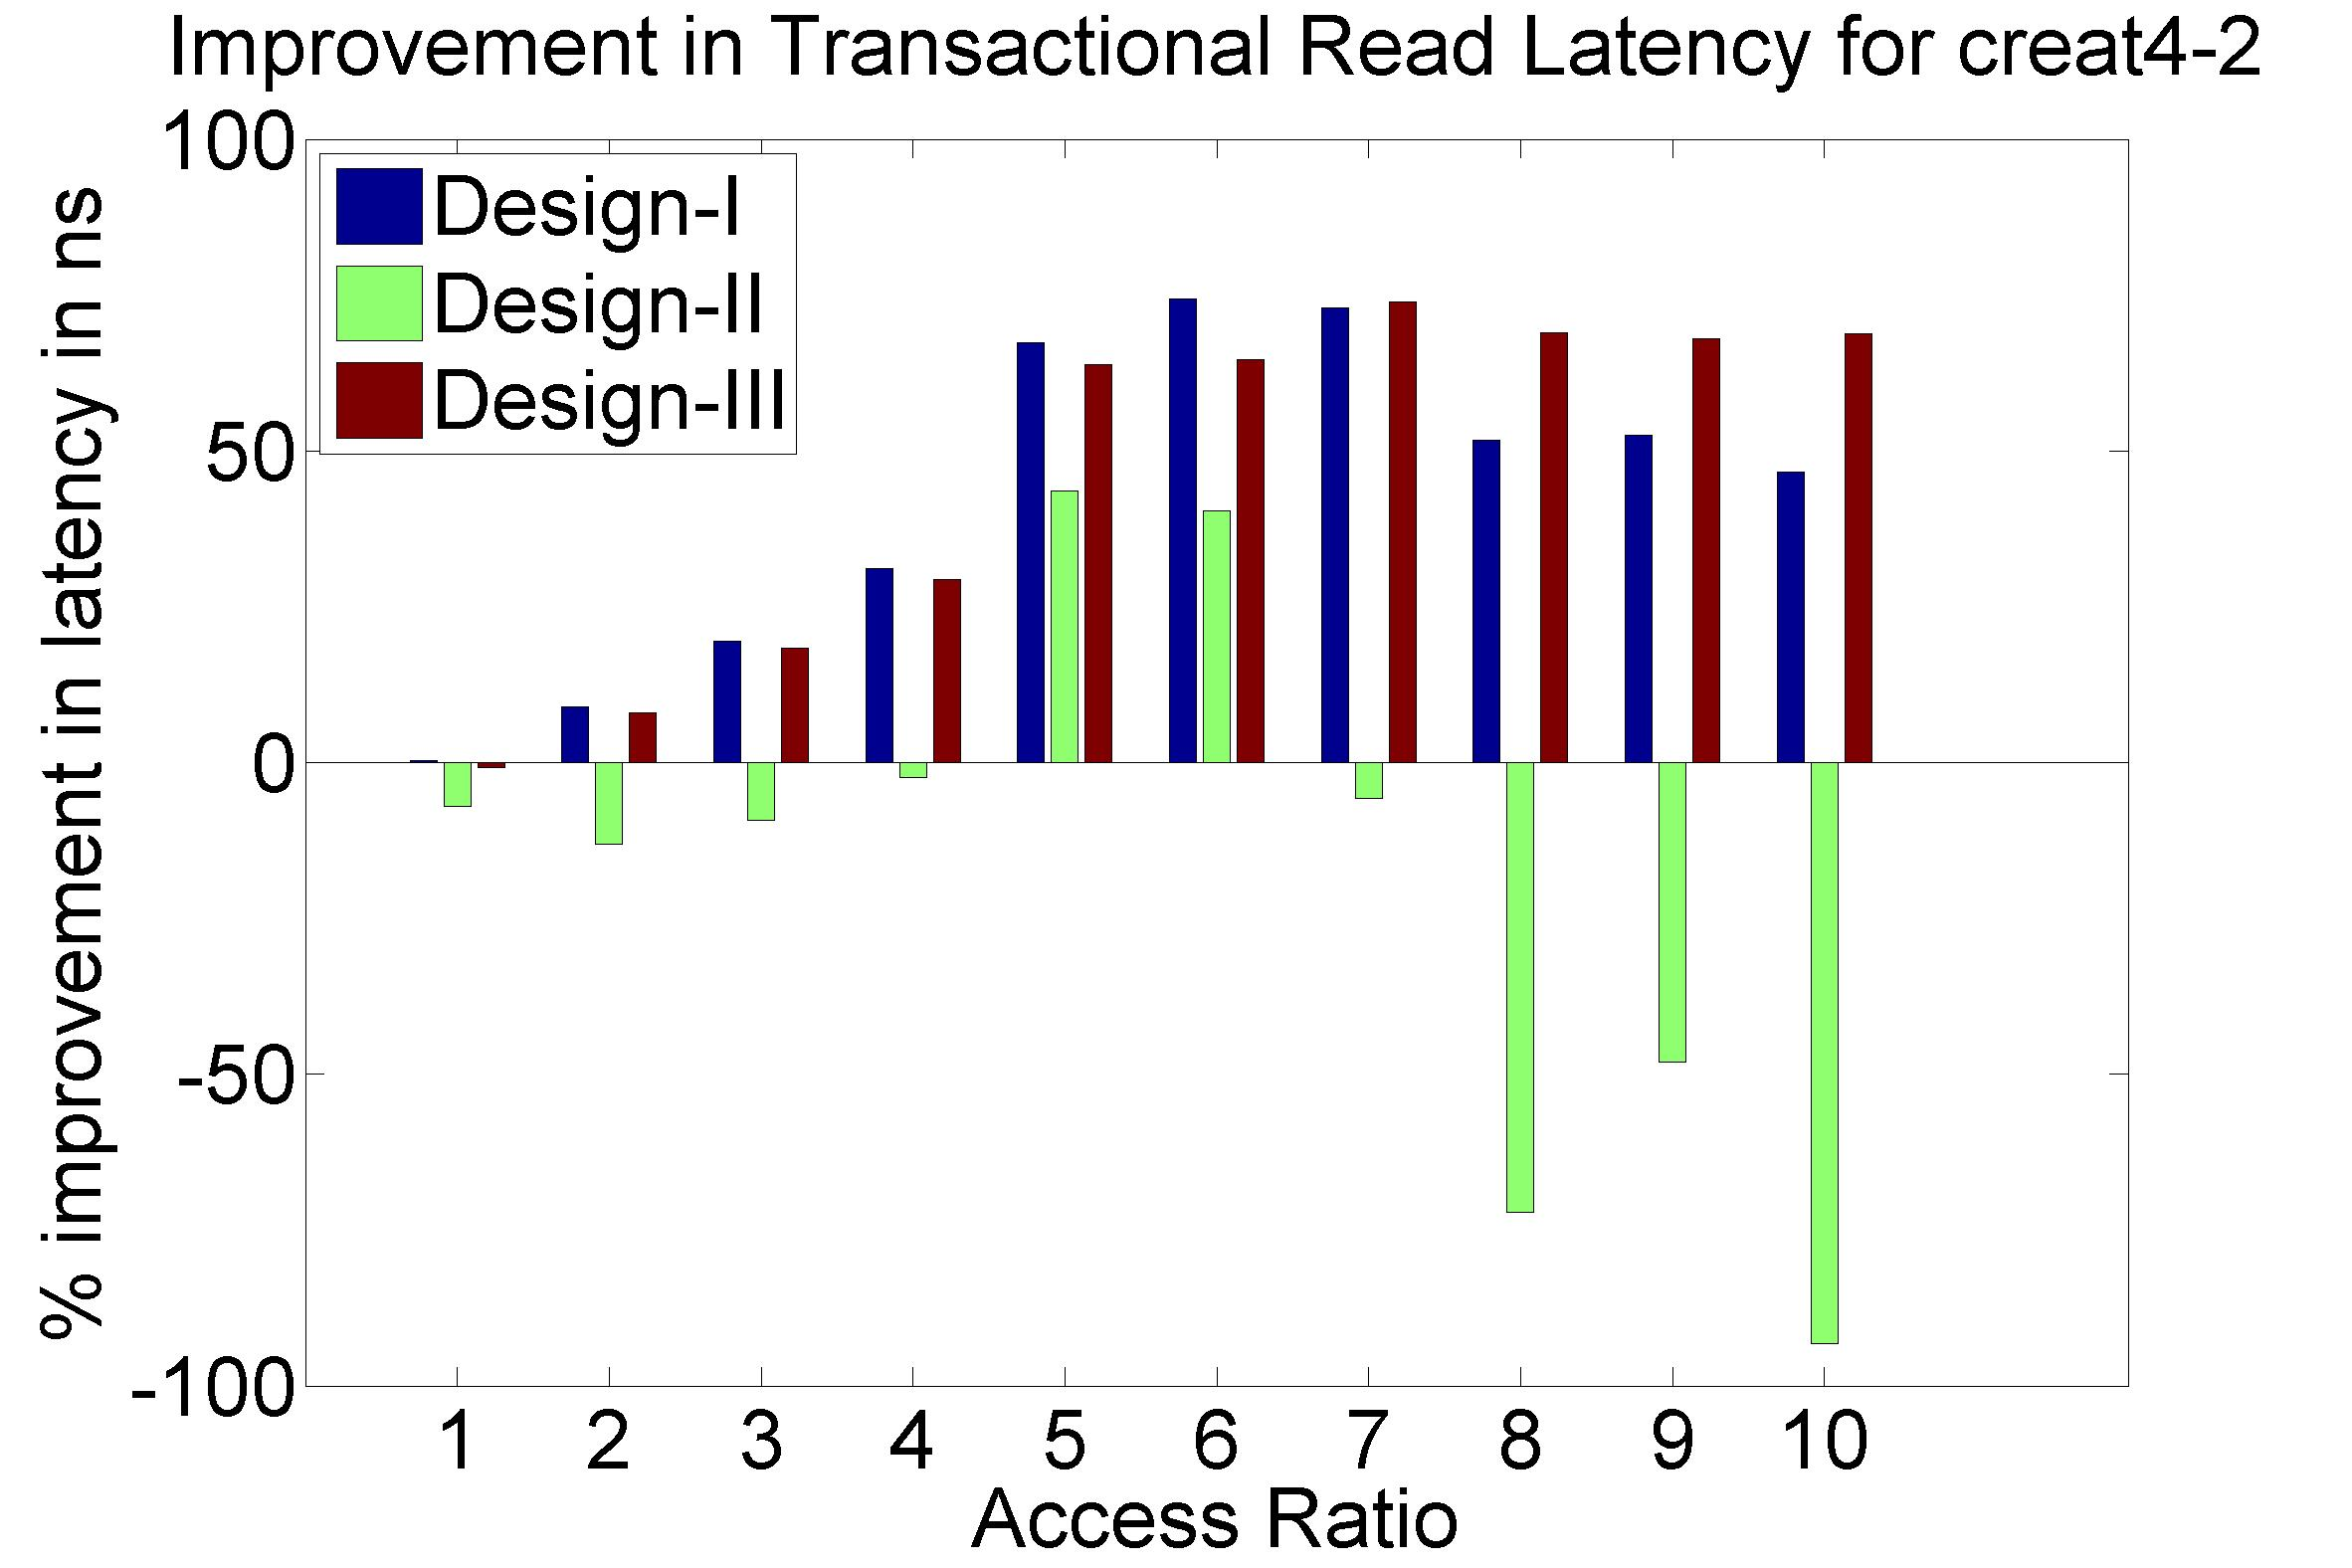
\includegraphics[width=\linewidth]{creat4-2_transactional_latency_improvement.jpeg}
\end{minipage}
\begin{minipage}[!t]{0.33\linewidth}
        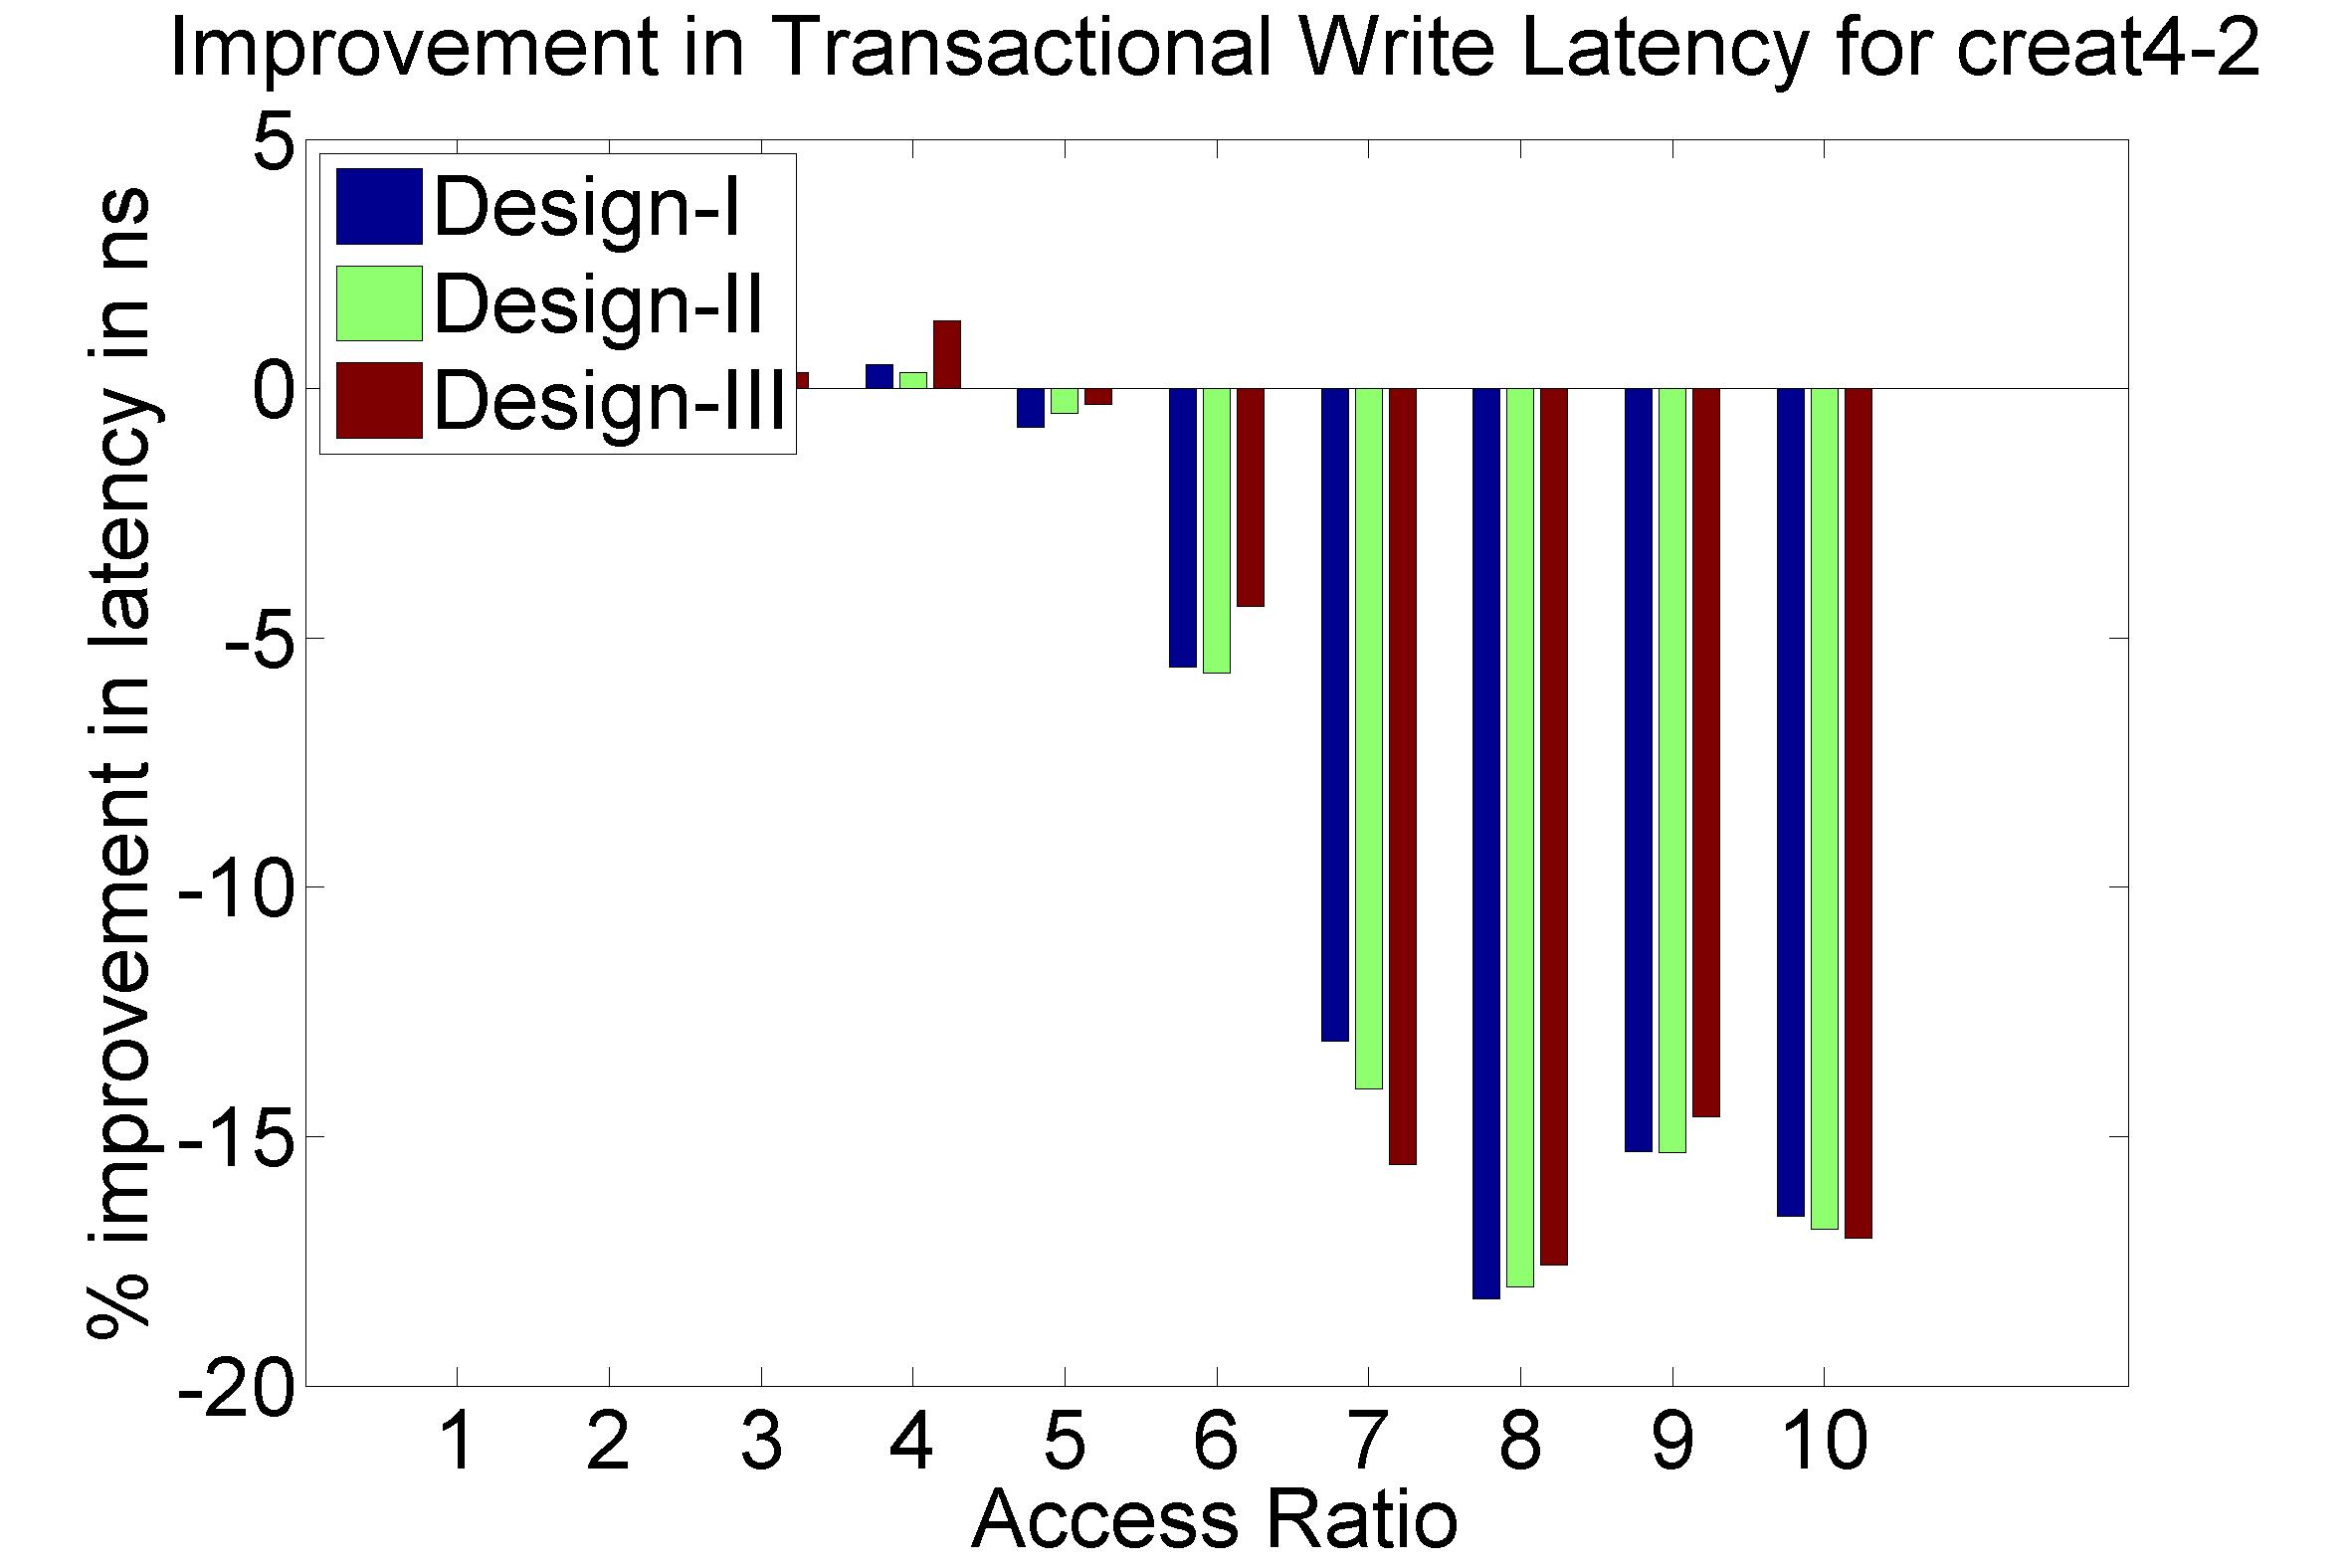
\includegraphics[width=\linewidth]{creat4-2_write_latency_improvement.jpeg}
\end{minipage}
\caption{
{\bf Performance Graphs for Creat4-2 trace} }
\label{fig:creat42_improvement}
\end{figure}
%-------------------------------------------------
Observations:
\begin{itemize}
	\item This trace is second part of Creat4 trace.creat4-2 is a medium density trace. 
	\item The improvement in critical read latency and transactional read latency is significant in design I and design III. 
	\item The write latency is positive till access ratio of 5.
	\item Design I and Design III codes benefit in this trace.
\end{itemize}
\cleardoublepage
%-------------------------------------------------
\begin{figure}[htb]
\begin{minipage}[!t]{\linewidth}
        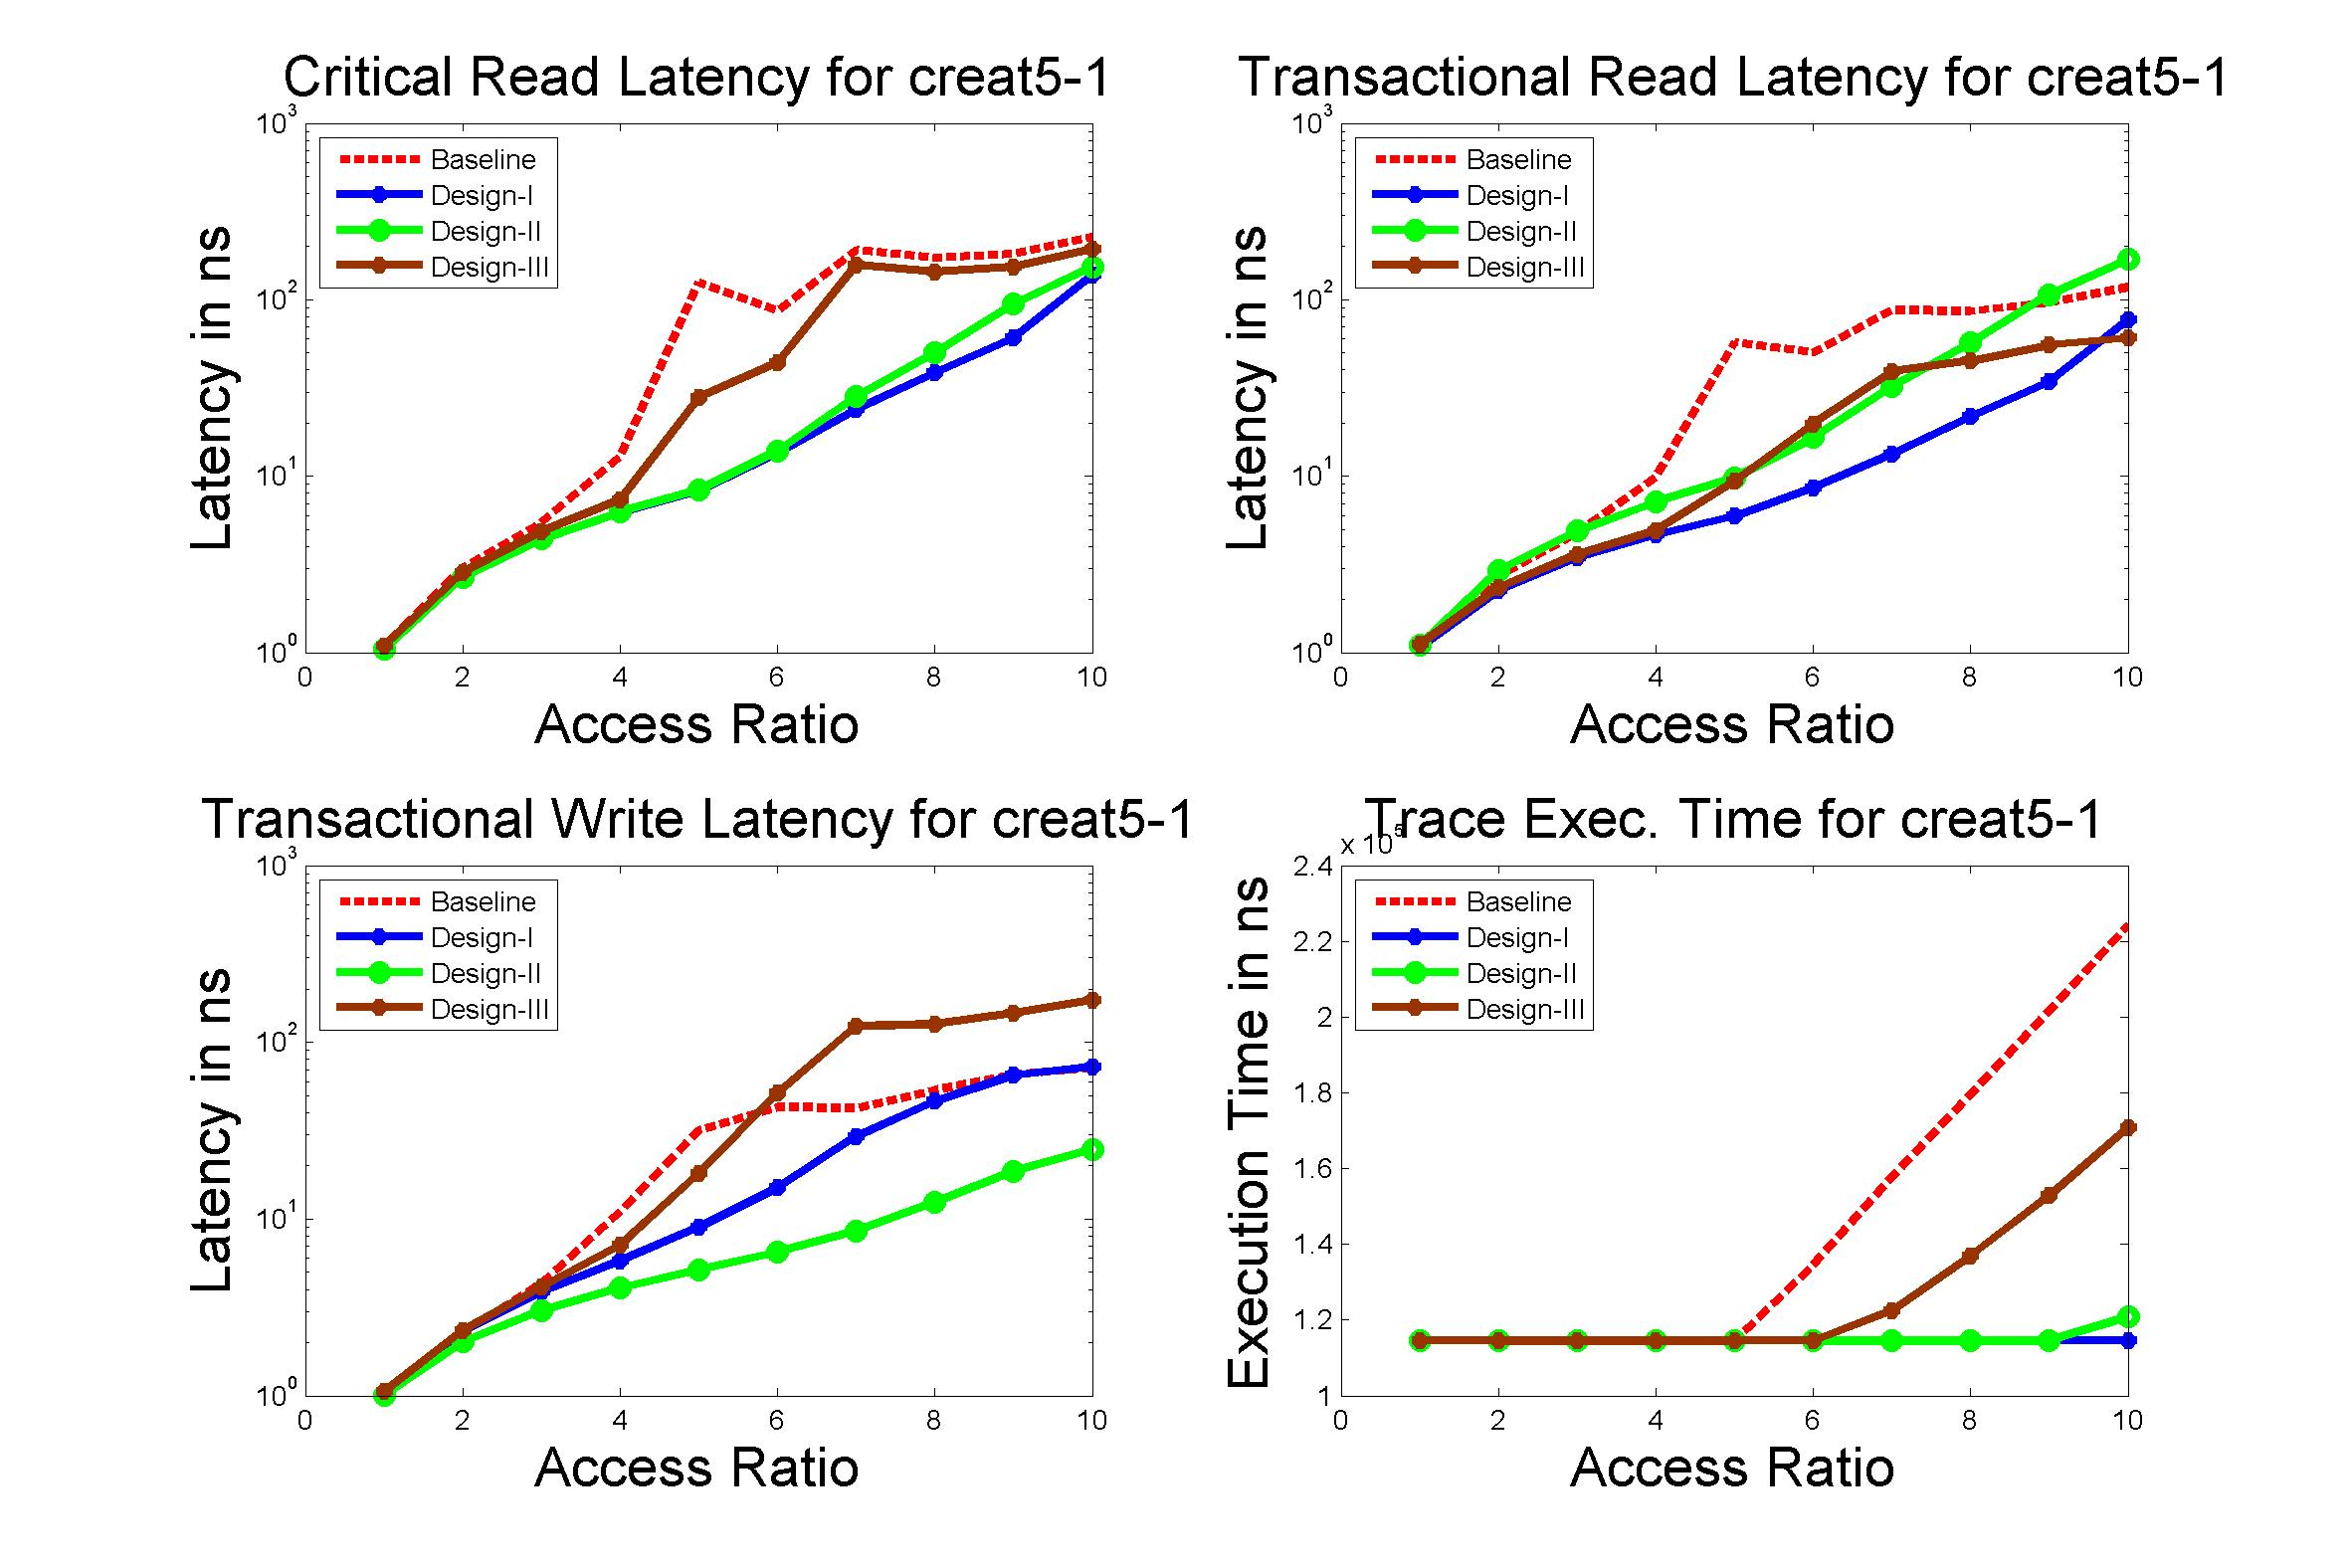
\includegraphics[width=\linewidth]{creat5-1.jpg}
\end{minipage}
\caption{
{\bf Performance Graphs for Creat5-1 trace} }
\label{fig:creat51}
\end{figure}
%-------------------------------------------------
\cleardoublepage
%-------------------------------------------------
\begin{figure}[htb]
	\centering
\begin{minipage}[!t]{0.32\linewidth}
        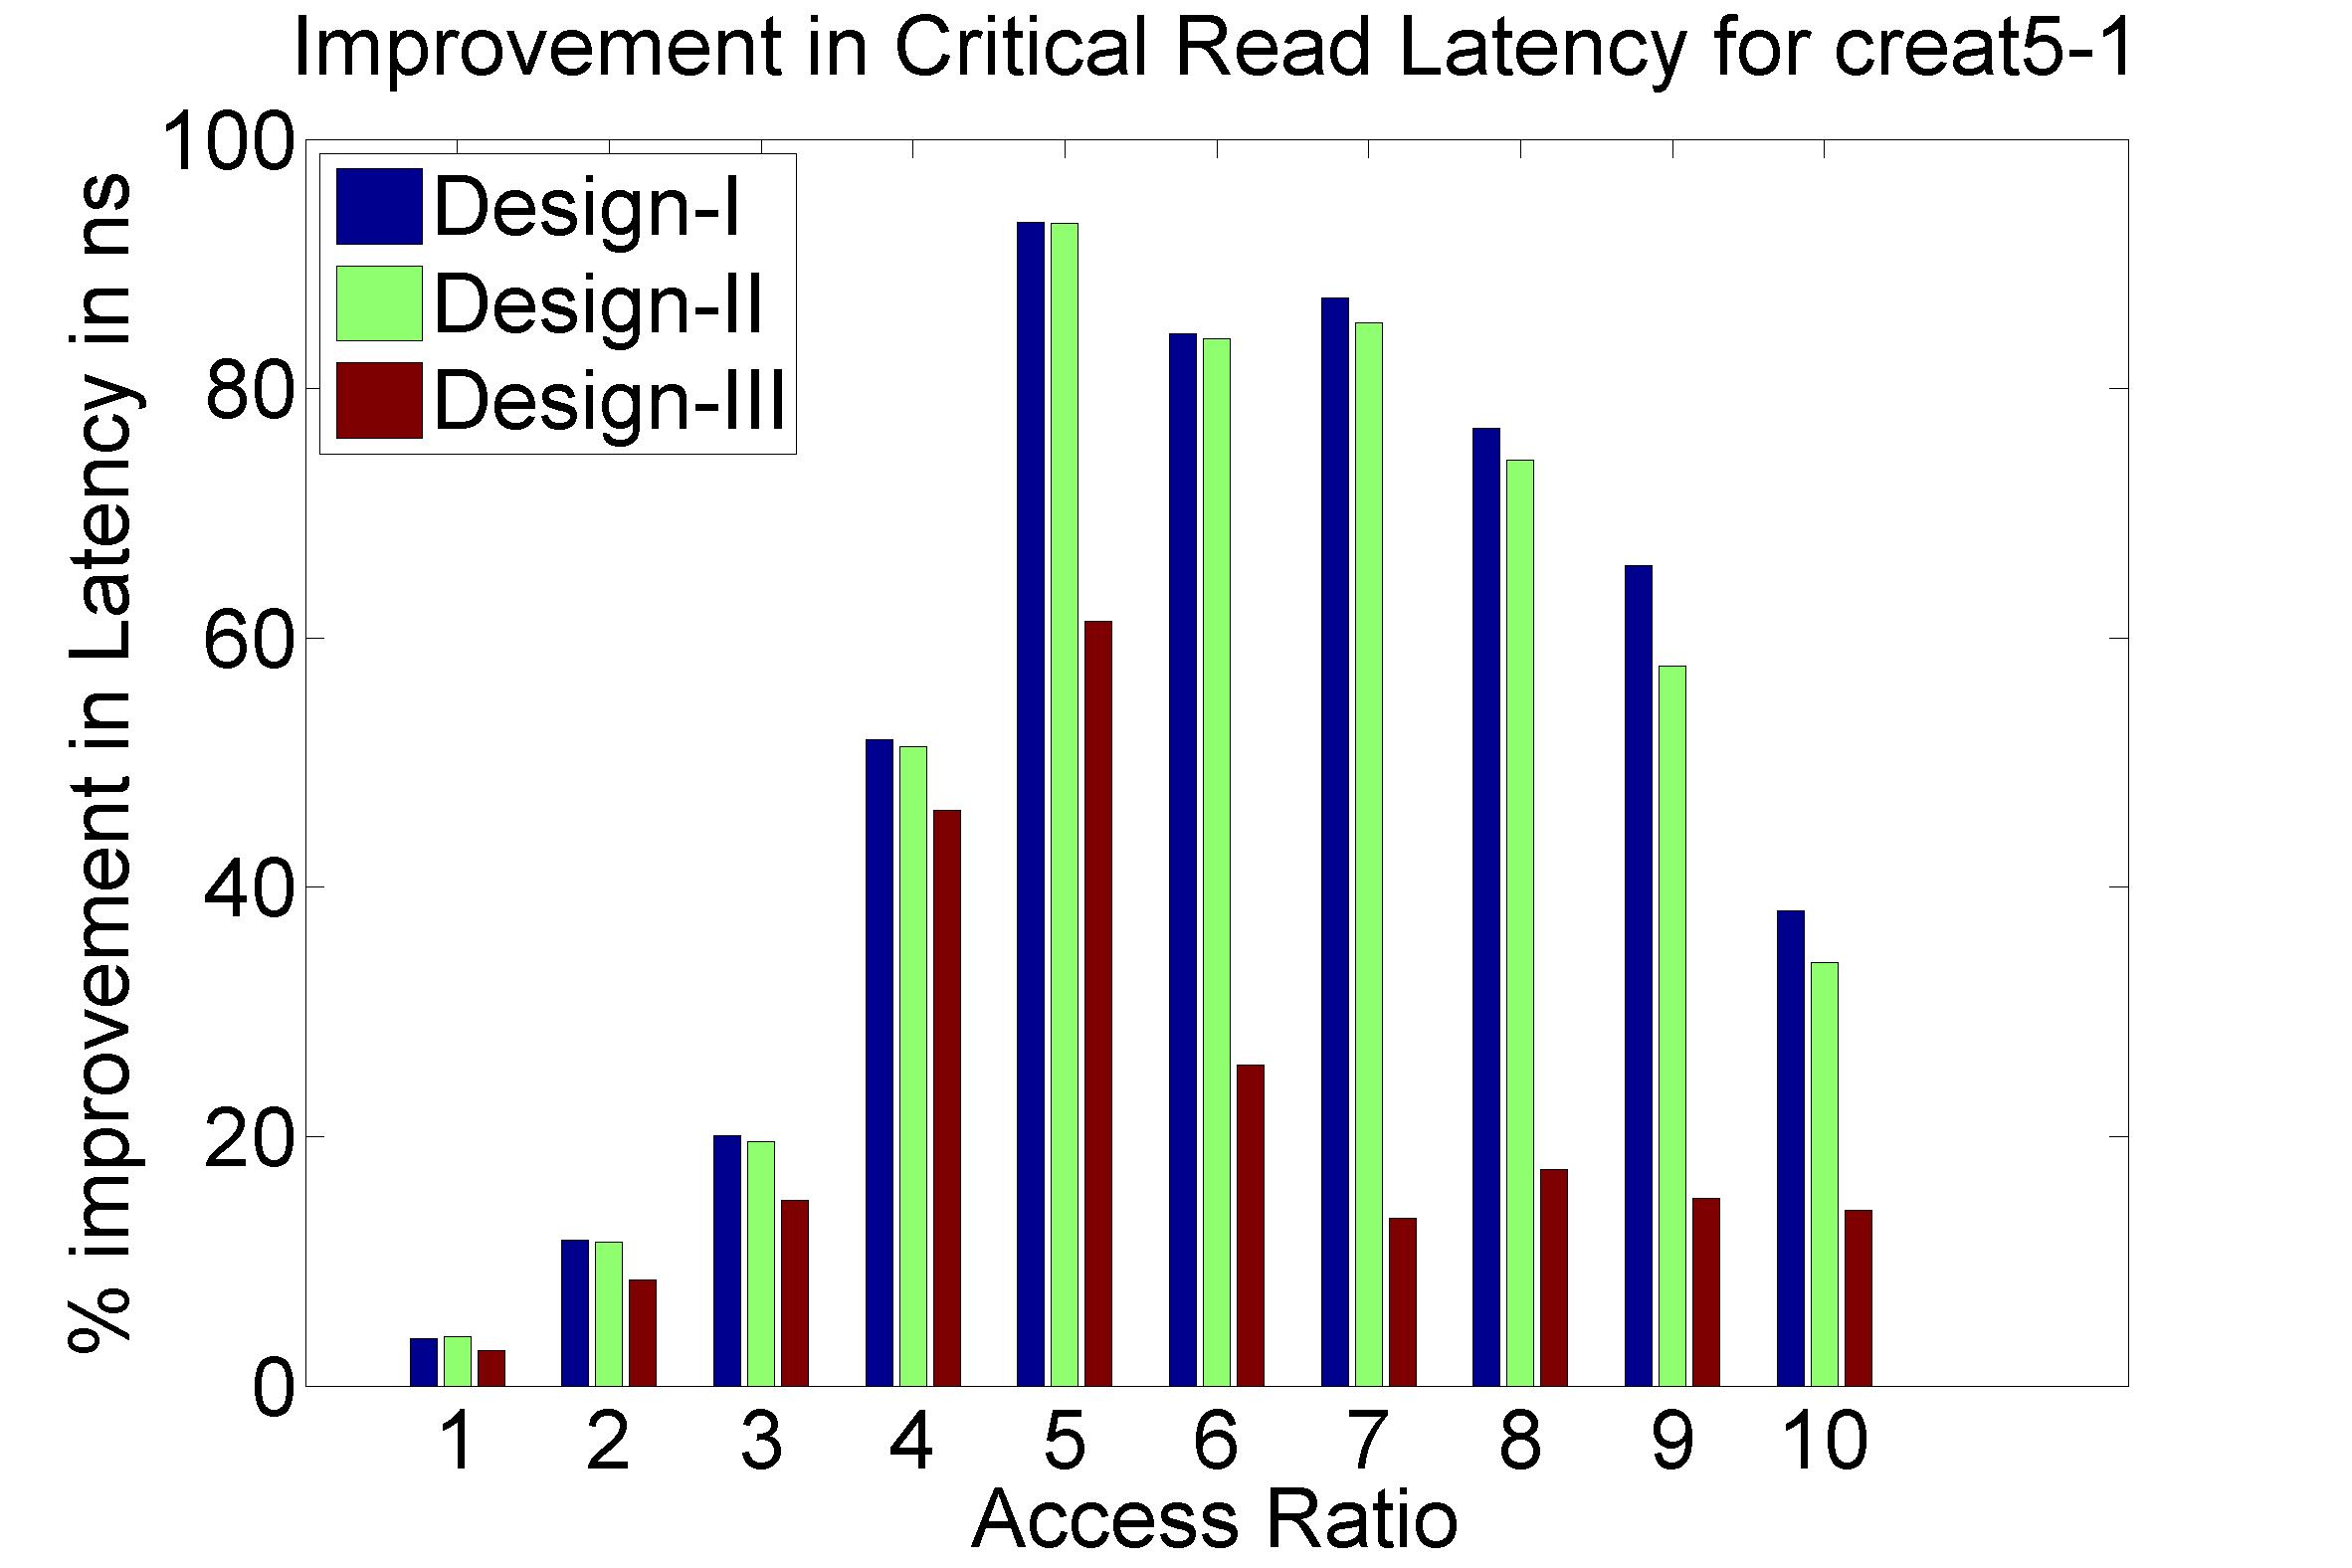
\includegraphics[width=\linewidth]{creat5-1_critical_latency_improvement.jpeg}
\end{minipage}
\begin{minipage}[!t]{0.32\linewidth}
        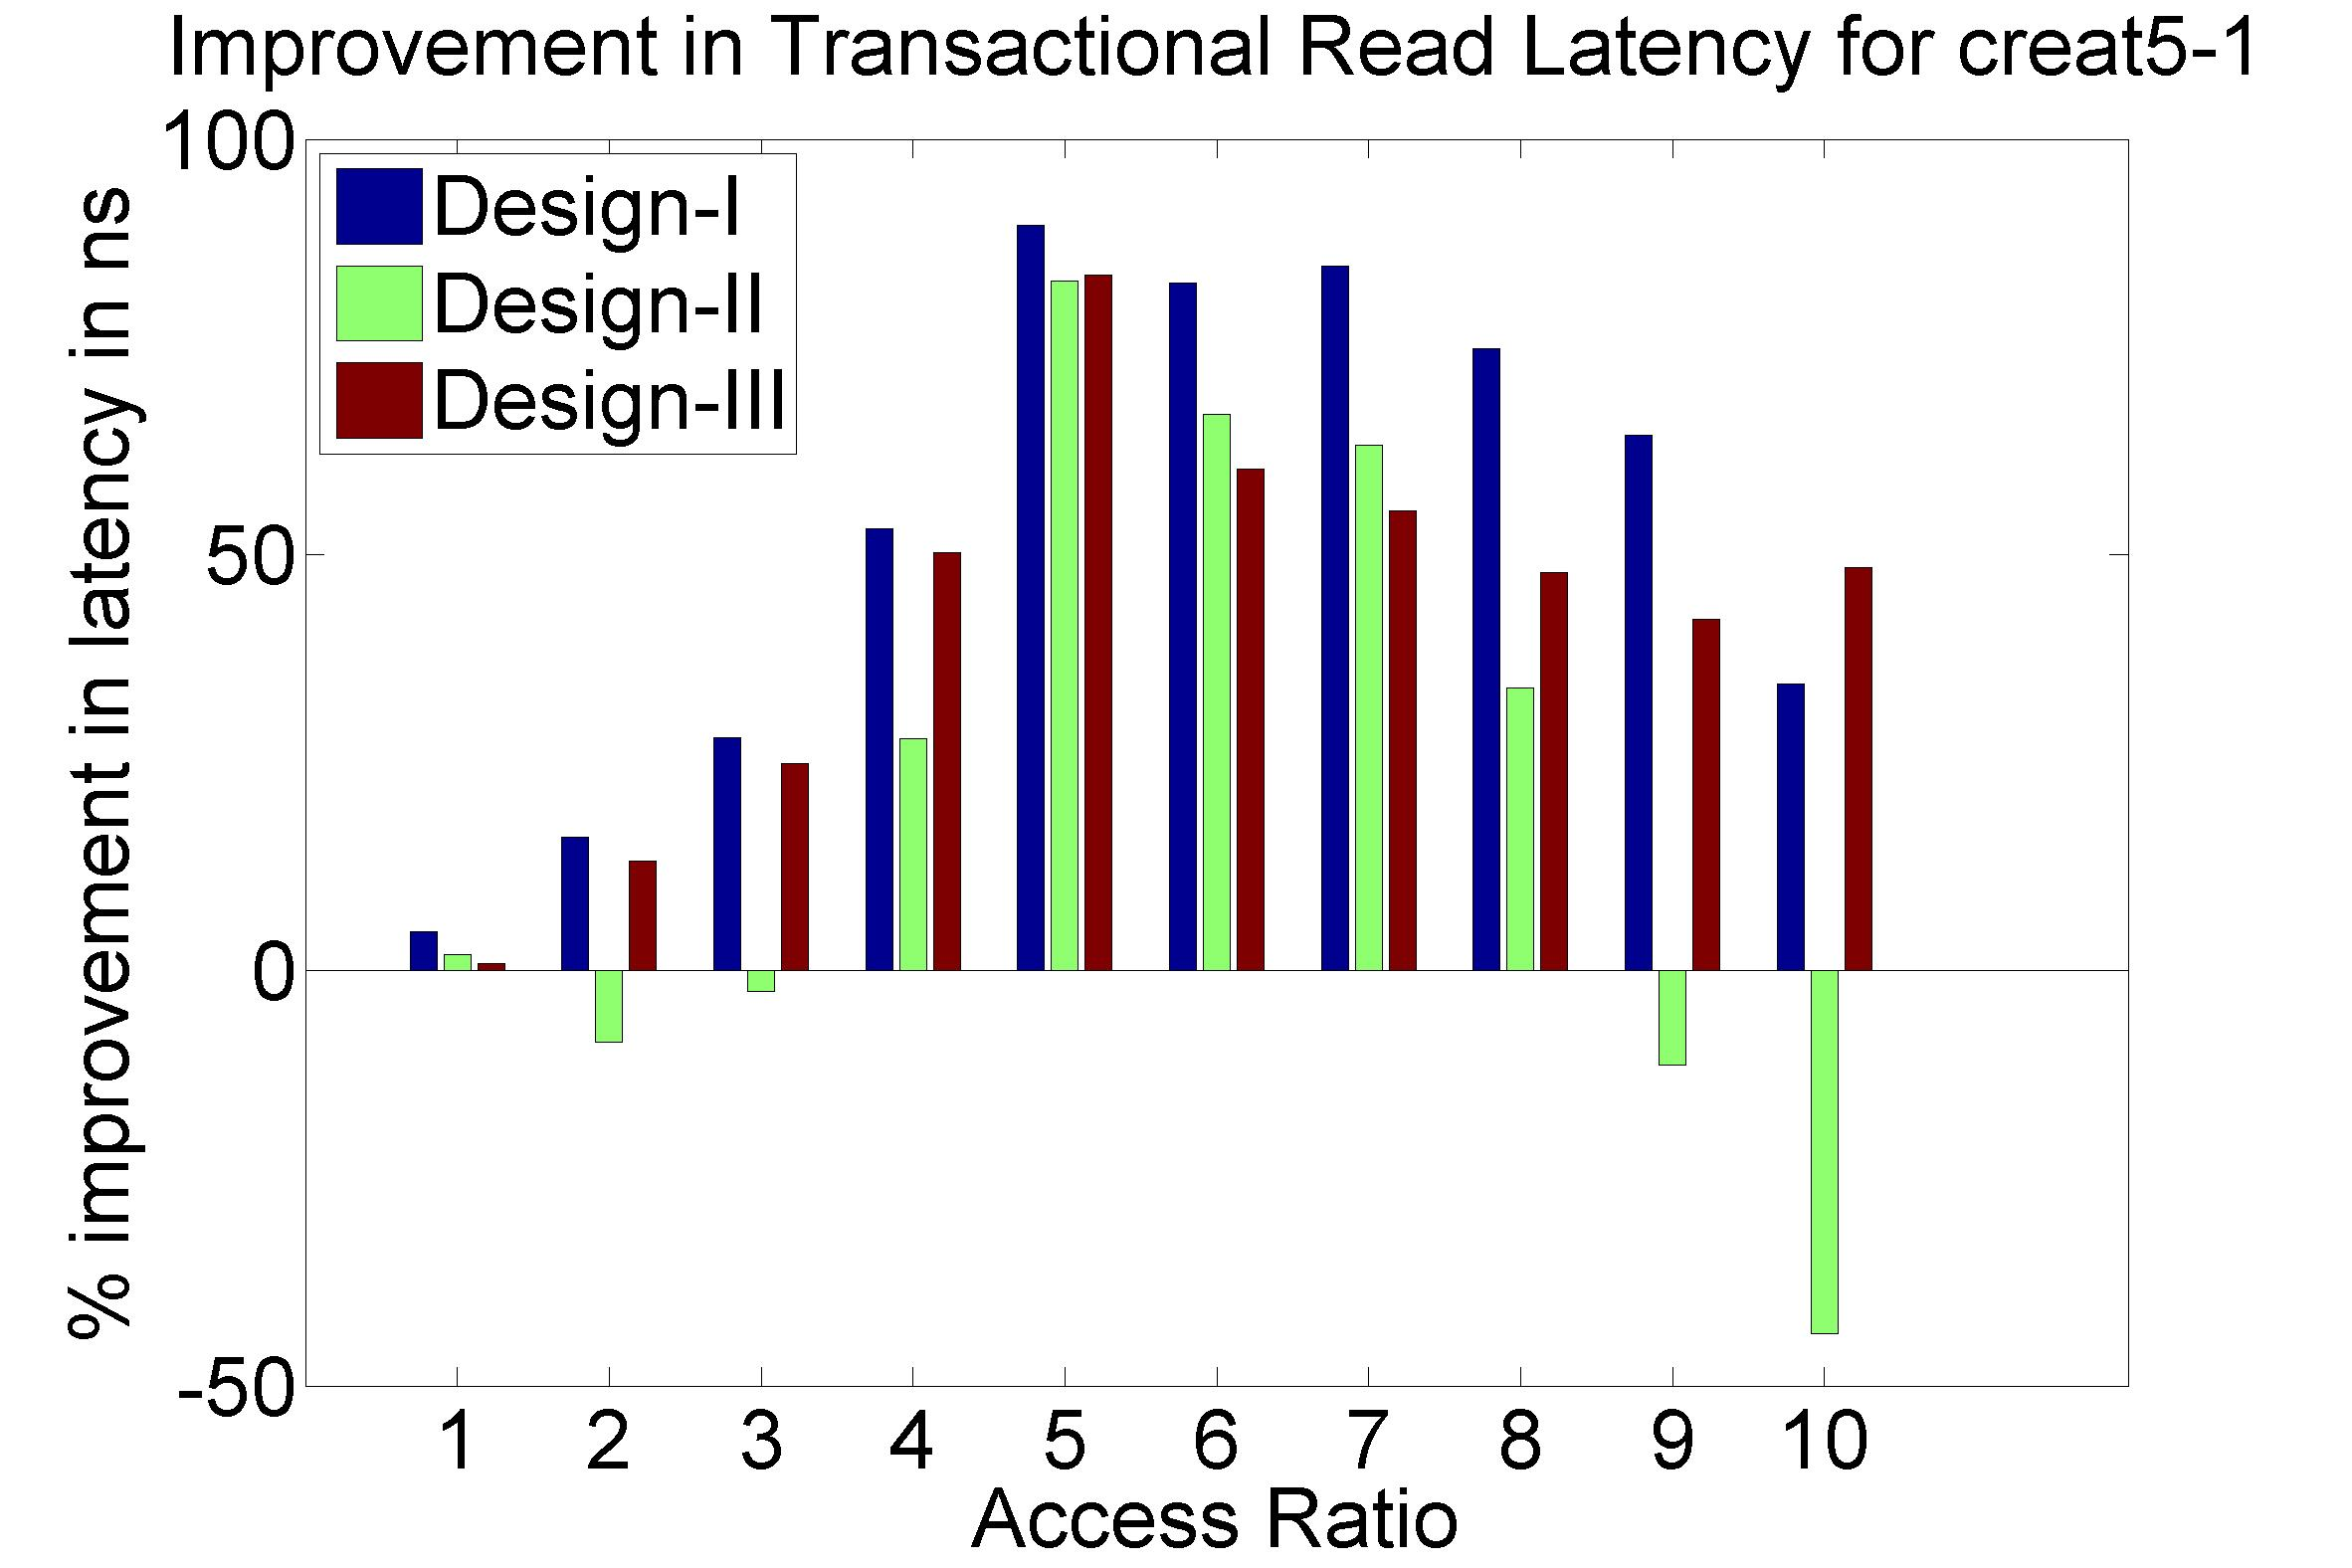
\includegraphics[width=\linewidth]{creat5-1_transactional_latency_improvement.jpeg}
\end{minipage}
\begin{minipage}[!t]{0.32\linewidth}
        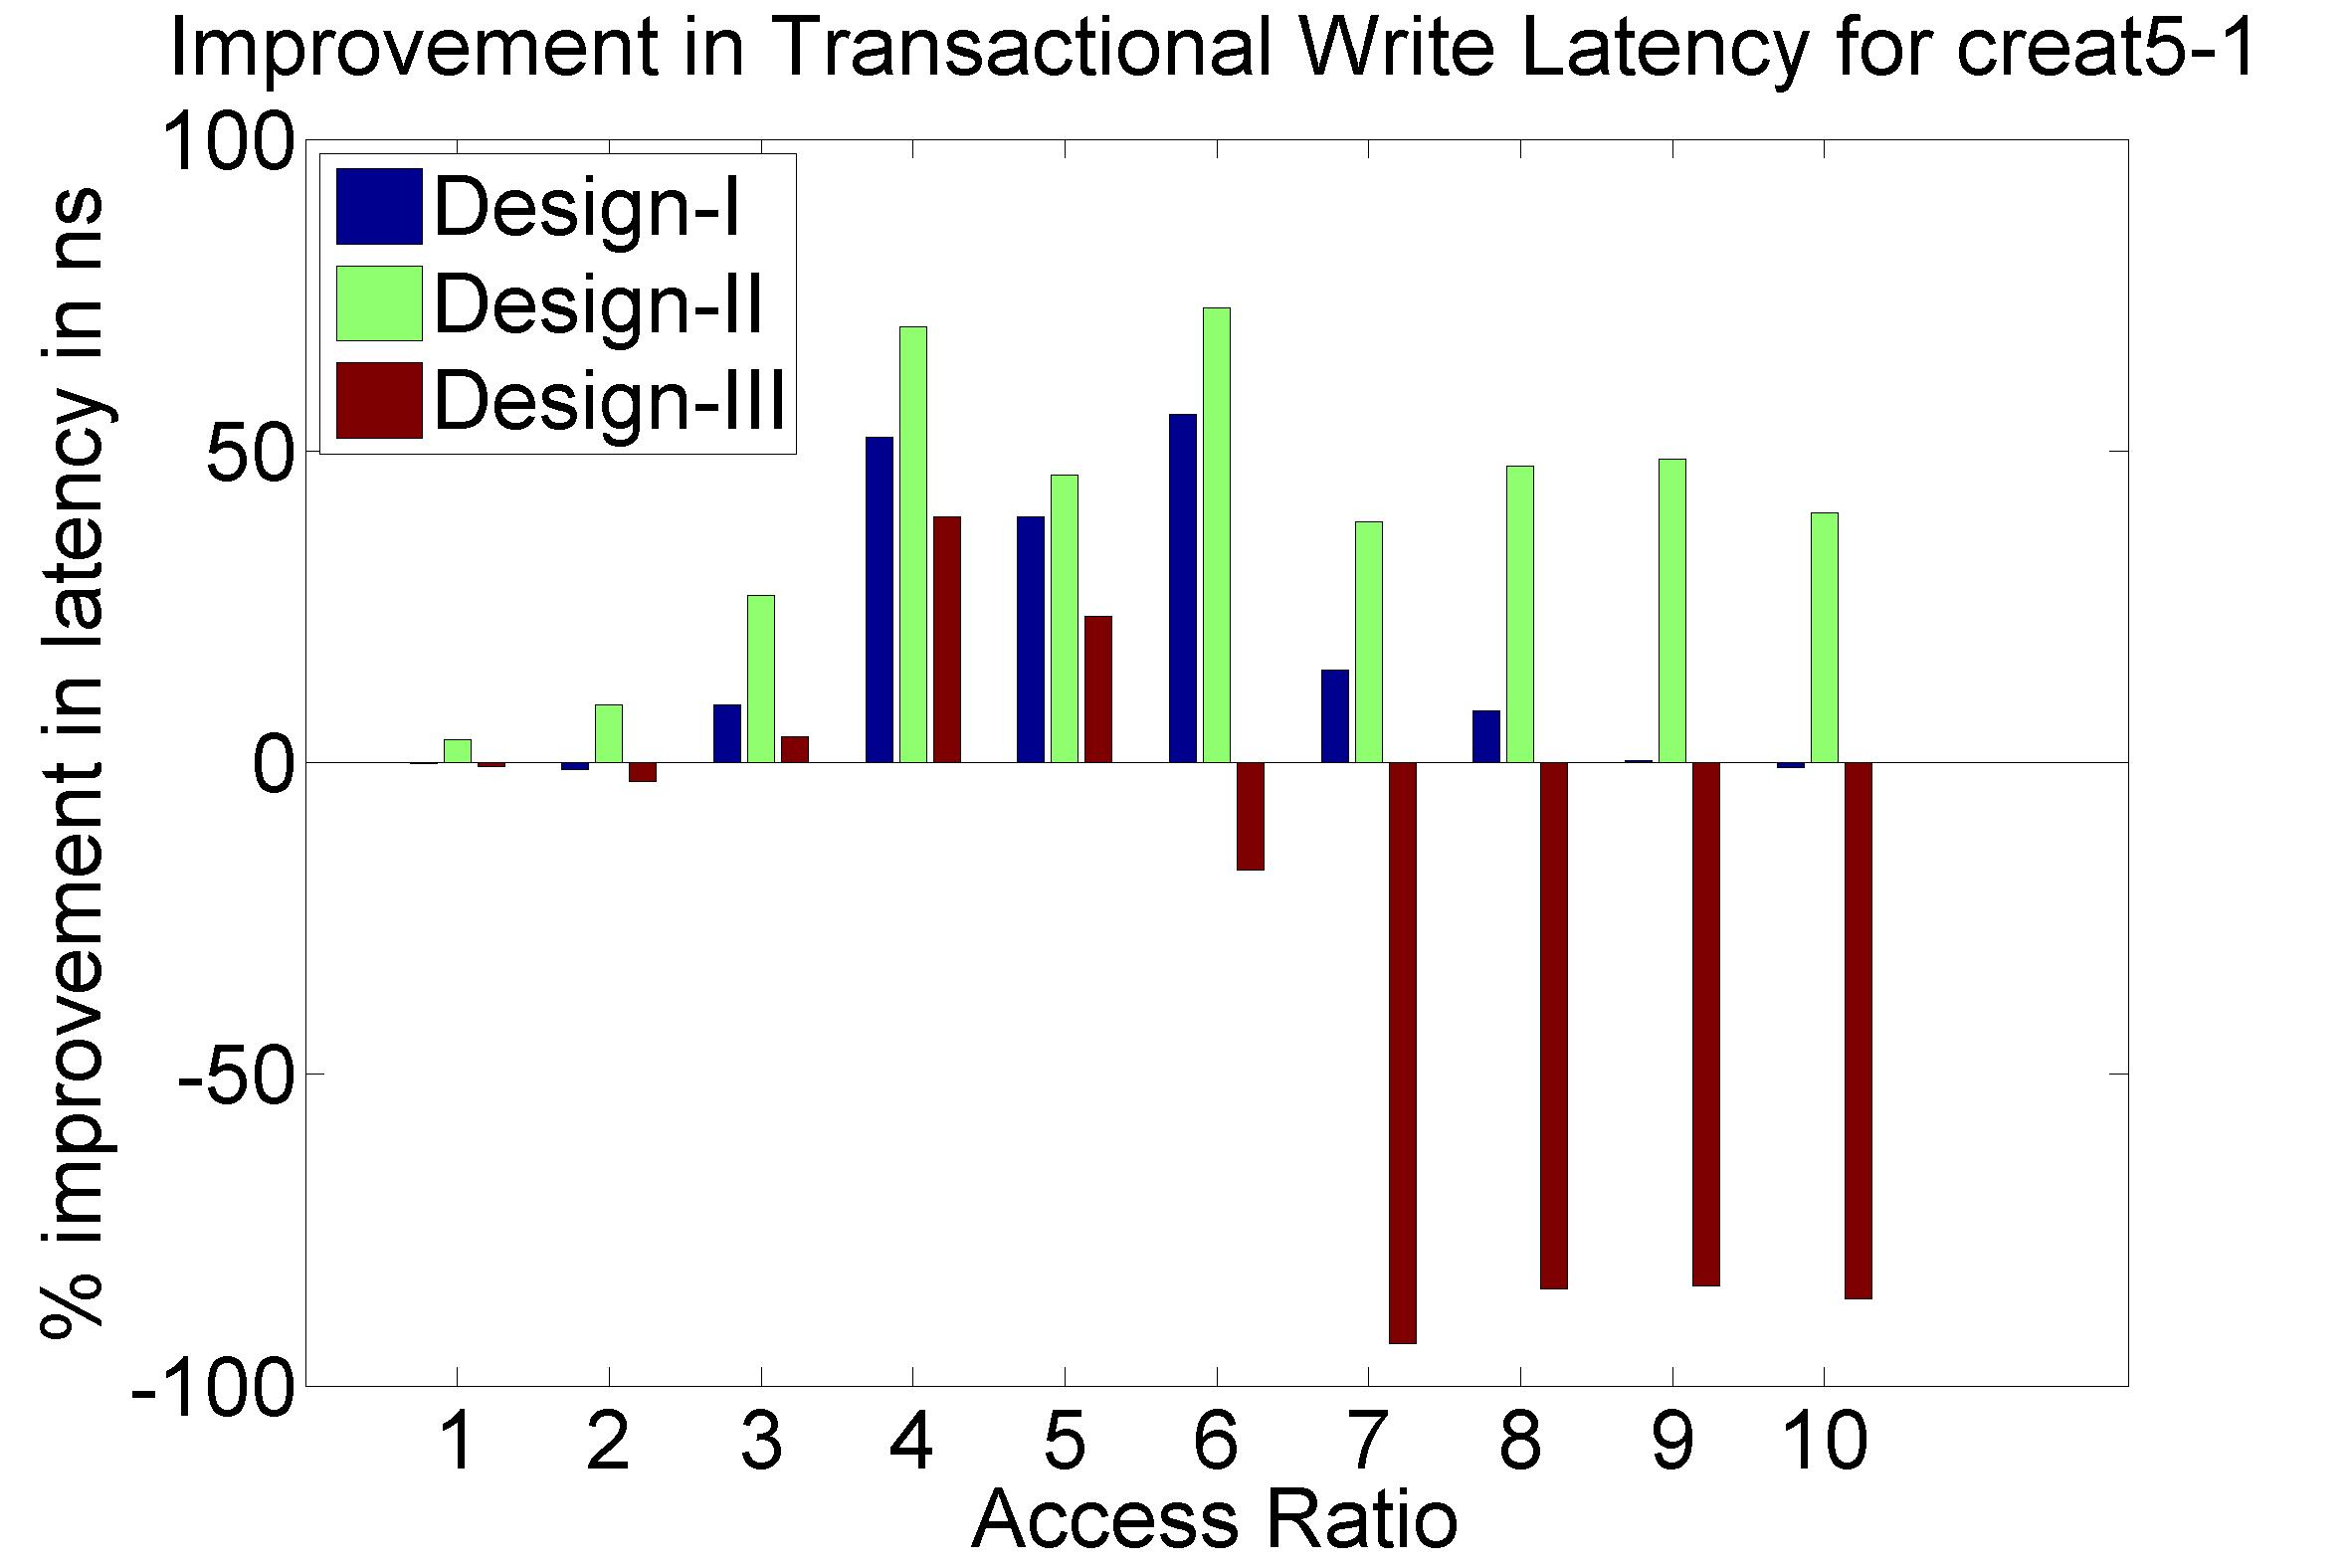
\includegraphics[width=\linewidth]{creat5-1_write_latency_improvement.jpeg}
\end{minipage}
\caption{
{\bf Performance Graphs for Creat5-1 trace} }
\label{fig:creat51_improvement}
\end{figure}
%-------------------------------------------------
Observations : 
\begin{itemize}
	\item Creat5-1 is a high density trace. 
	\item There is a significant critical read latency improvement for all access ratios in all design. 
	\item The transactional read latency is improves for all access ratios. 
	\item The write access latency improves for access ratio between 3 and 6.
	\item All the code designs are ideal for this trace. 
	\item Coding architecture is ideal for this trace.
\end{itemize}
\cleardoublepage
%-------------------------------------------------
\begin{figure}[htb]
\begin{minipage}[!t]{\linewidth}
        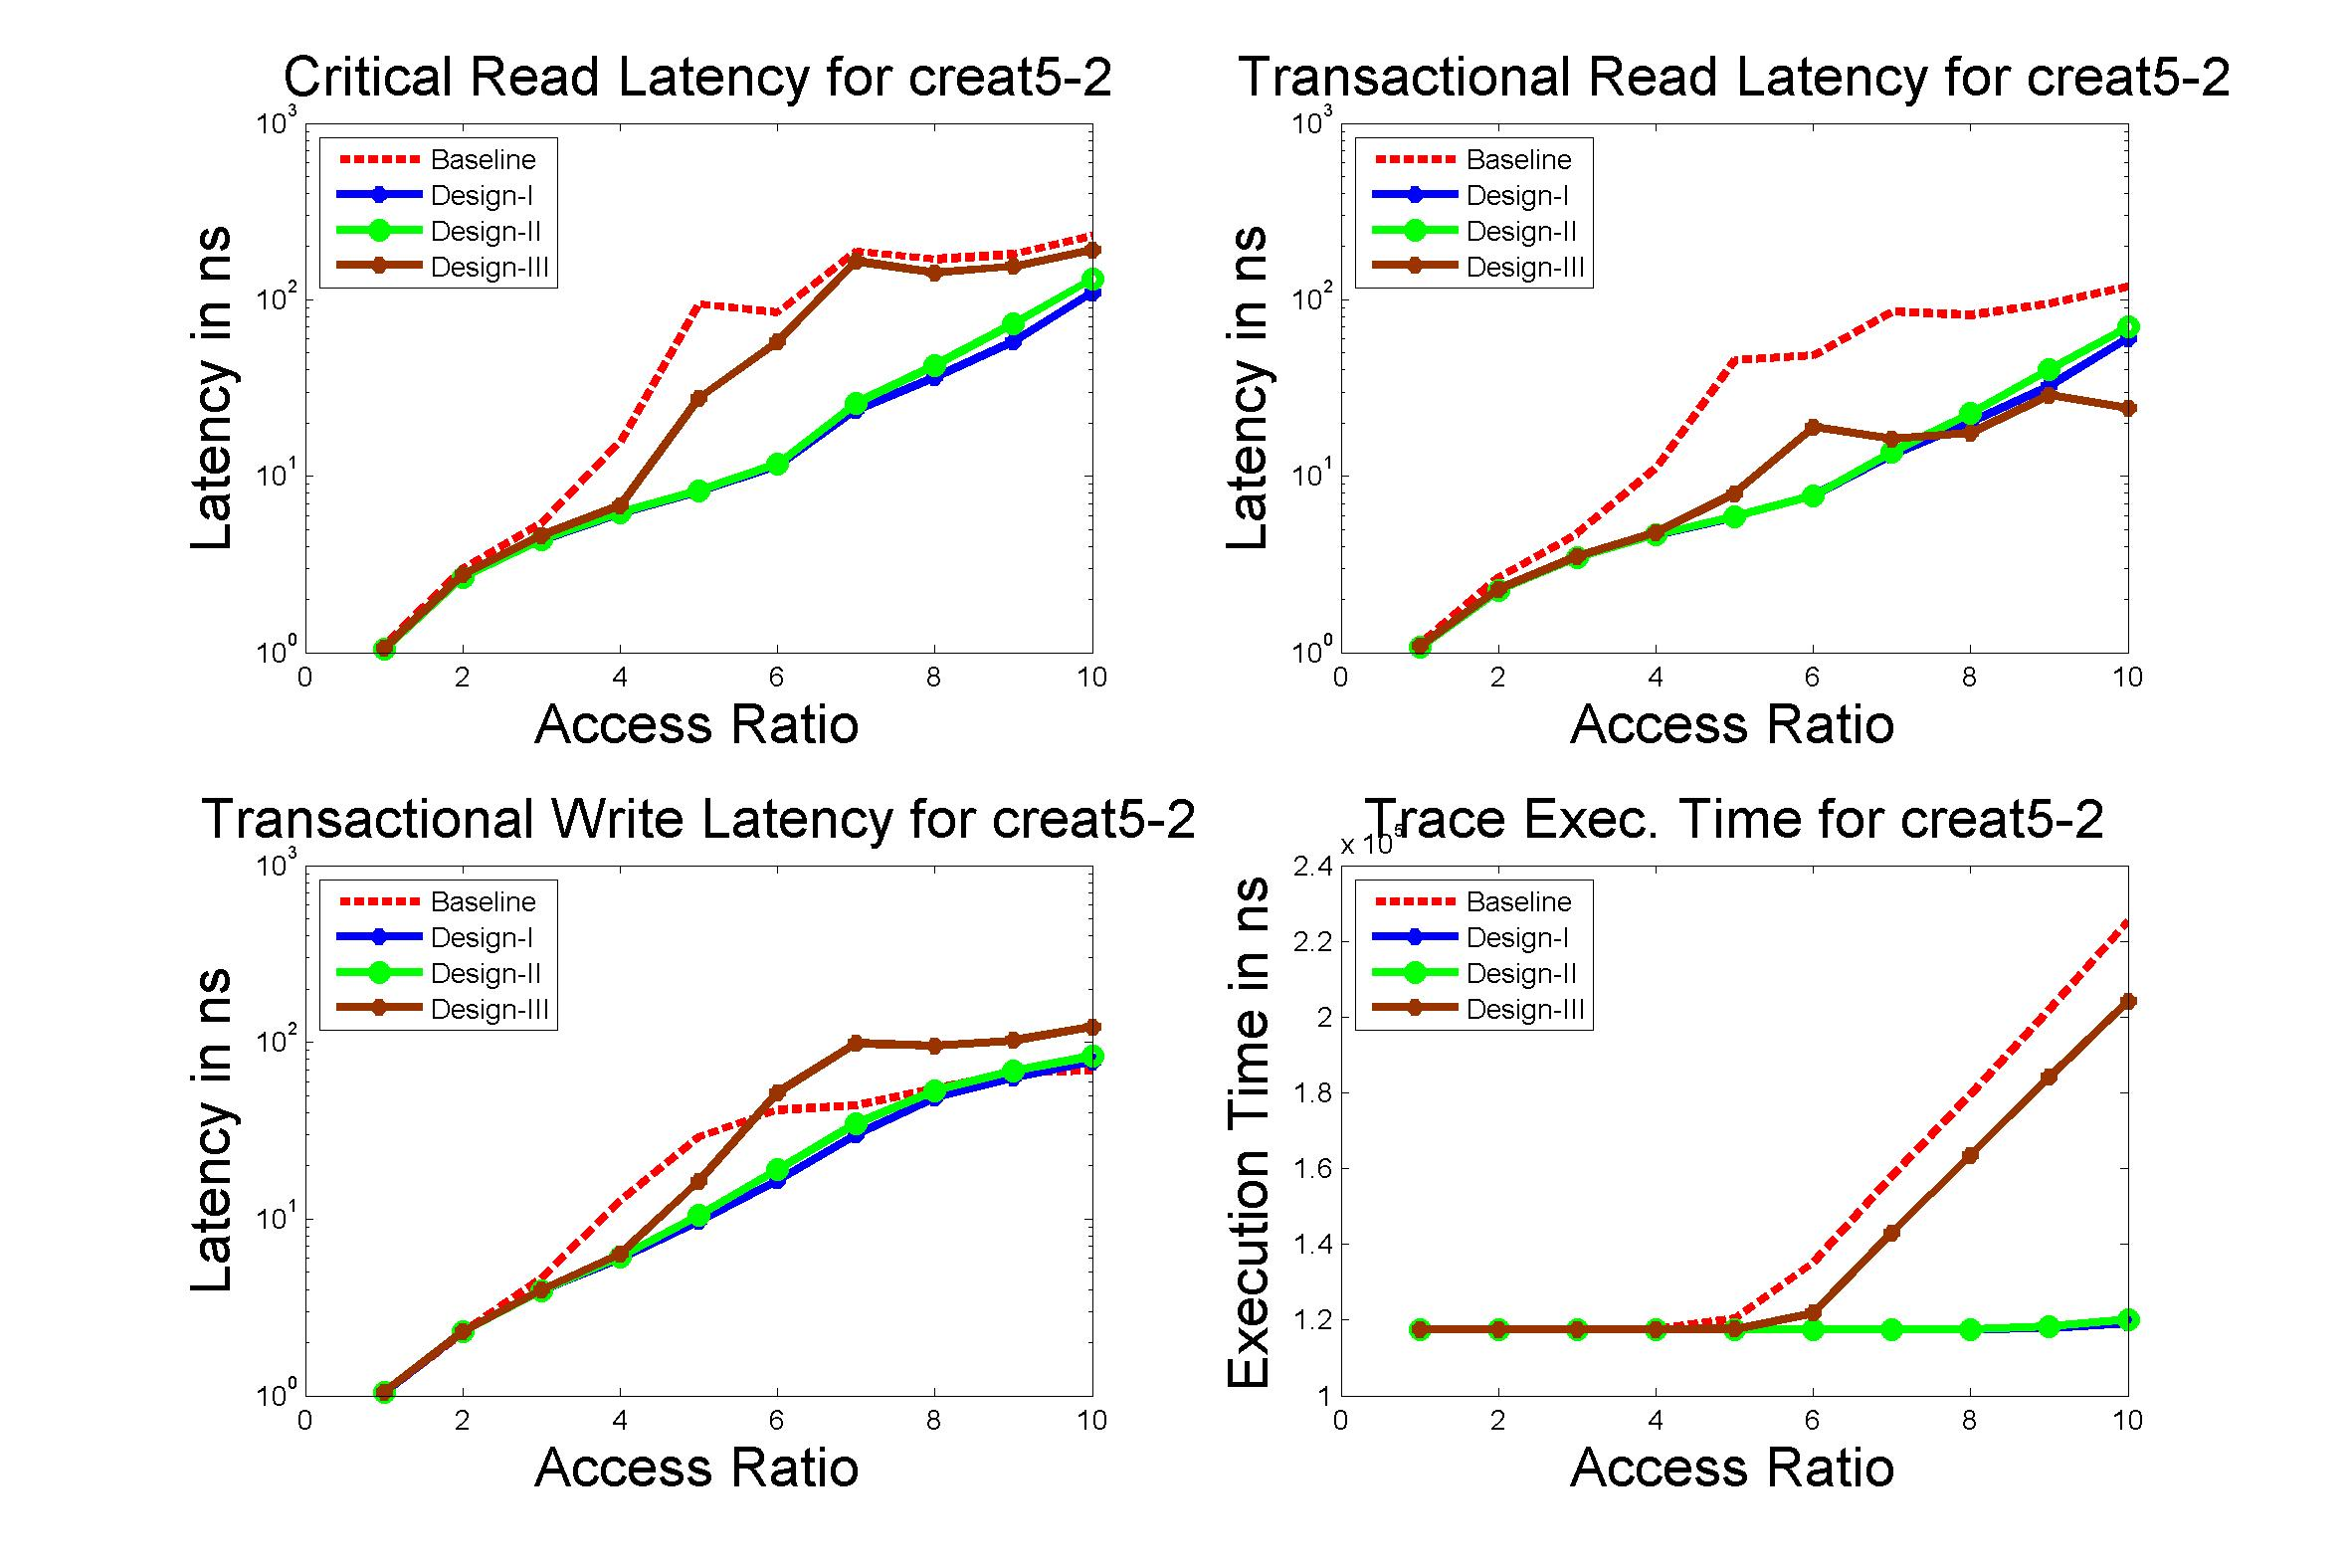
\includegraphics[width=\linewidth]{creat5-2.jpg}
\end{minipage}
\caption{
{\bf Performance Graphs for Creat5-2 trace} }
\label{fig:creat52}
\end{figure}
%-------------------------------------------------

\cleardoublepage
%-------------------------------------------------
\begin{figure}[htb]
	\centering
\begin{minipage}[!t]{0.32\linewidth}
        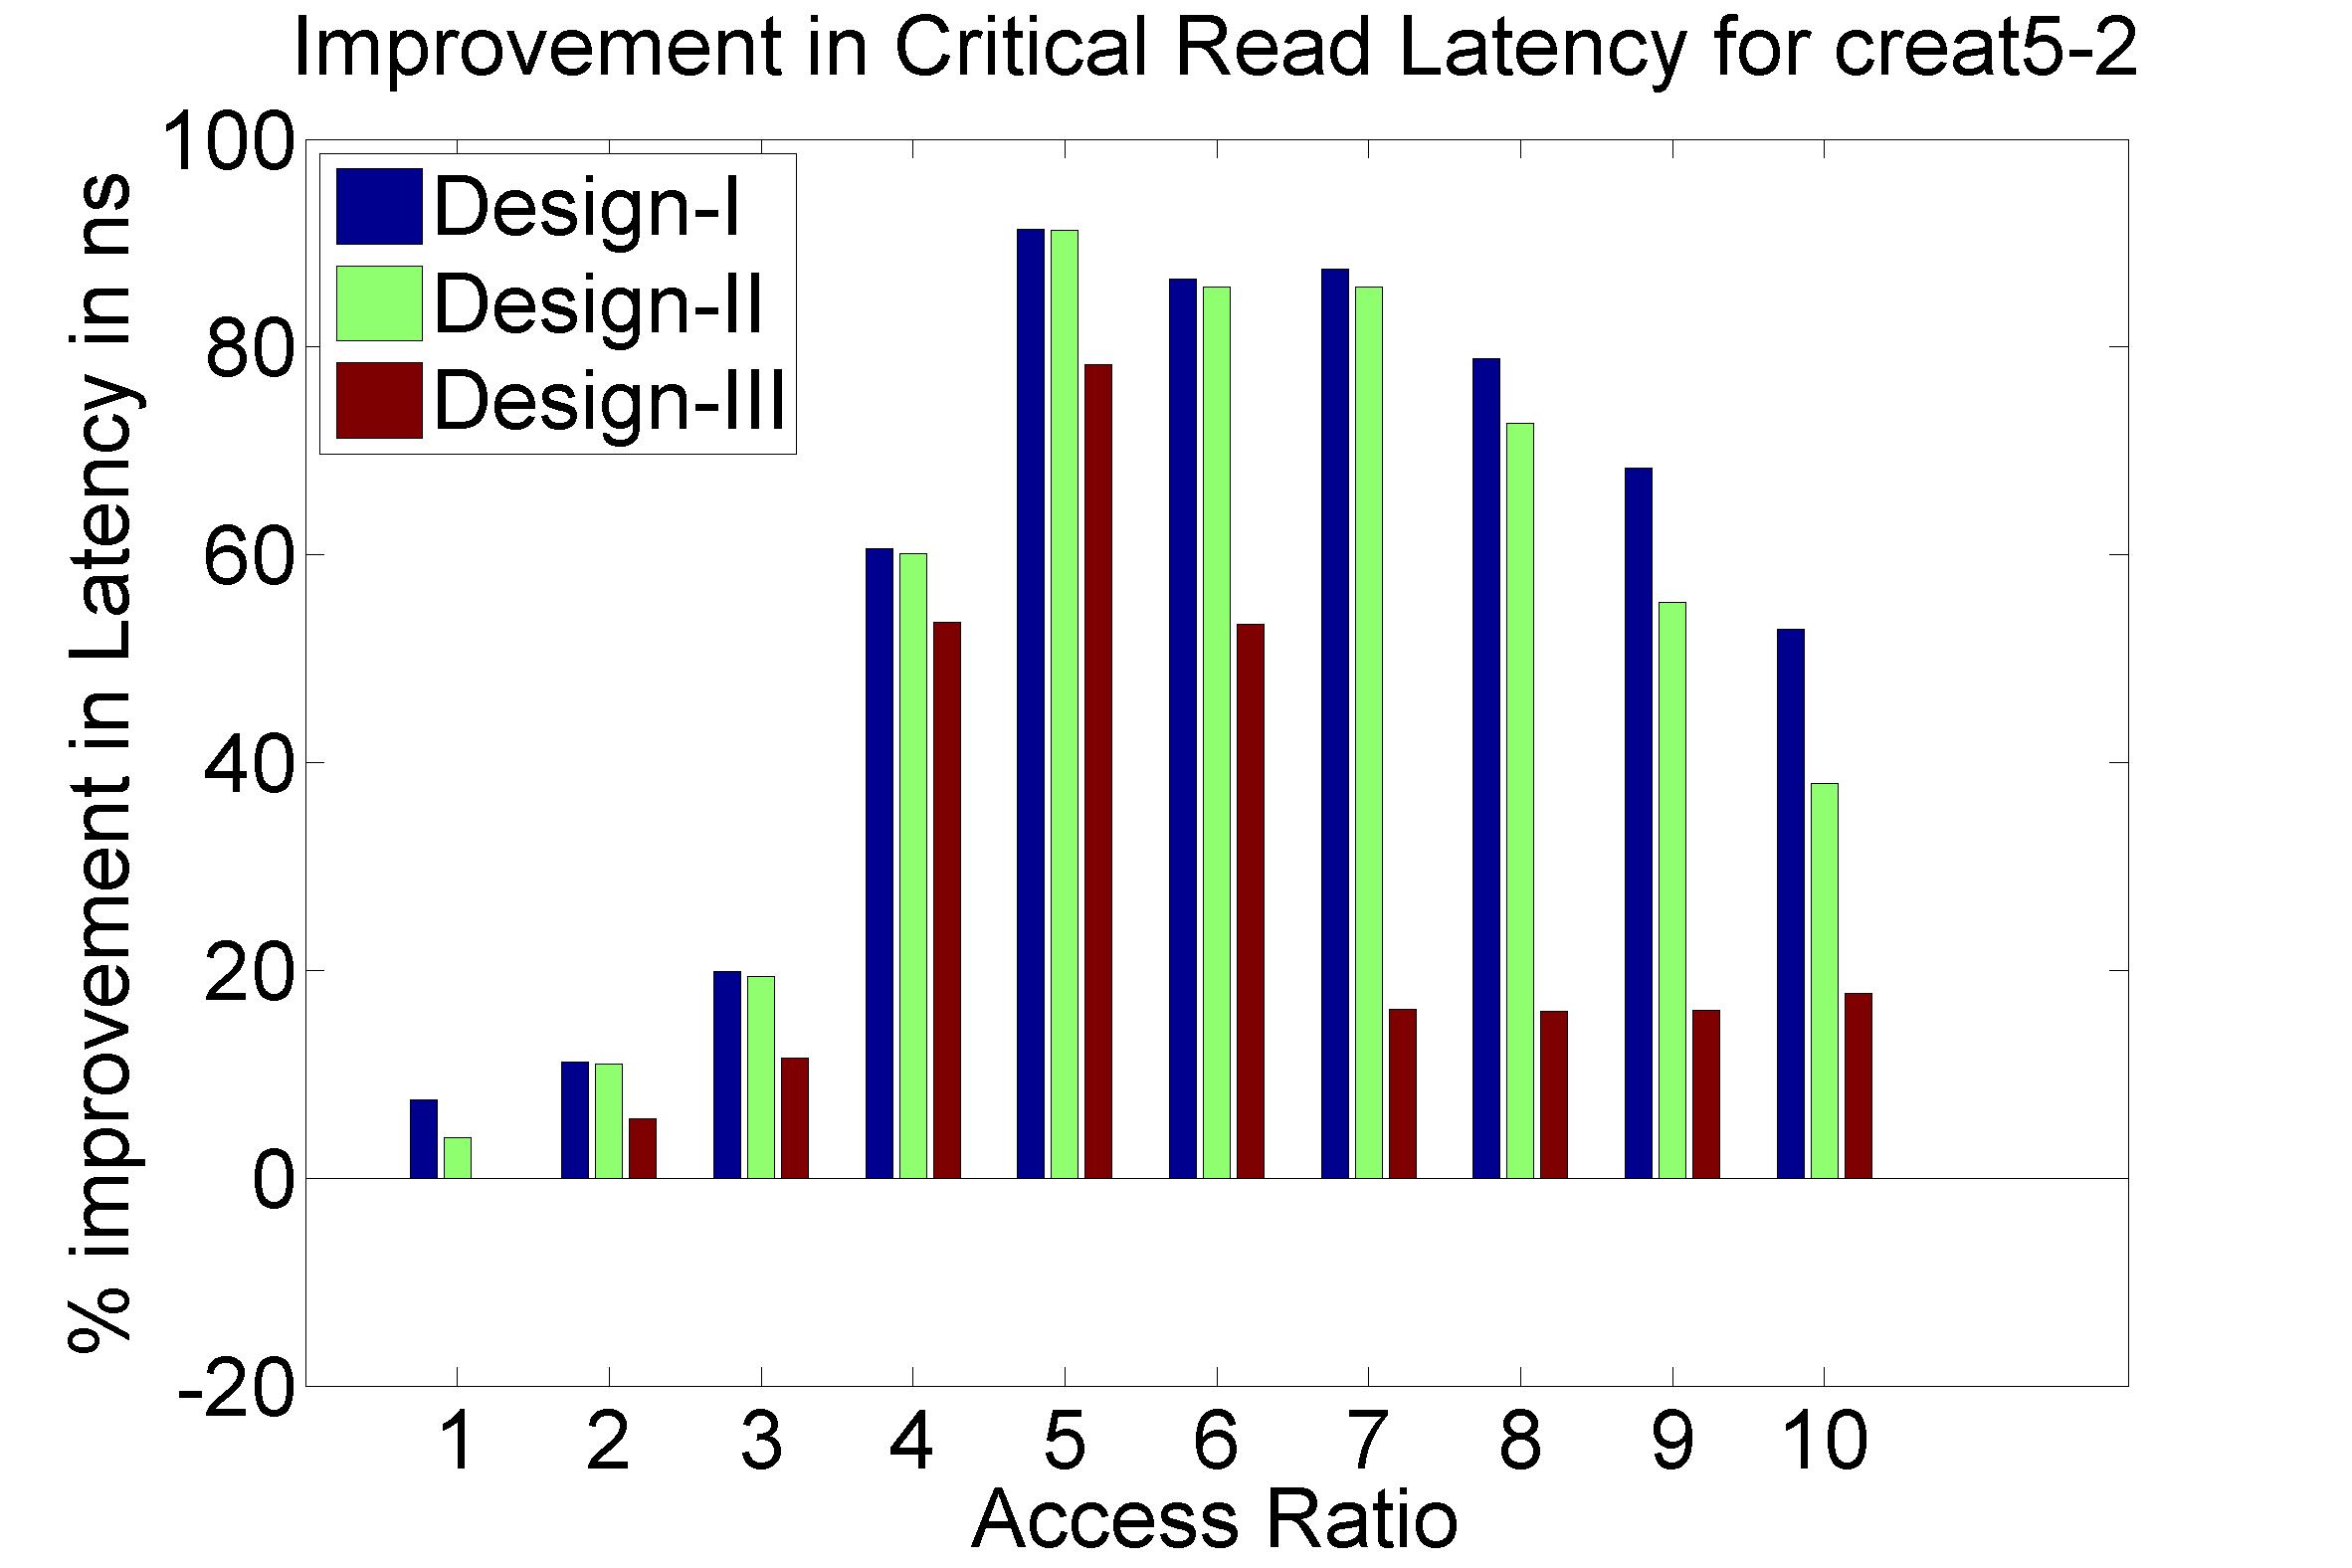
\includegraphics[width=\linewidth]{creat5-2_critical_latency_improvement.jpeg}
\end{minipage}
\begin{minipage}[!t]{0.32\linewidth}
        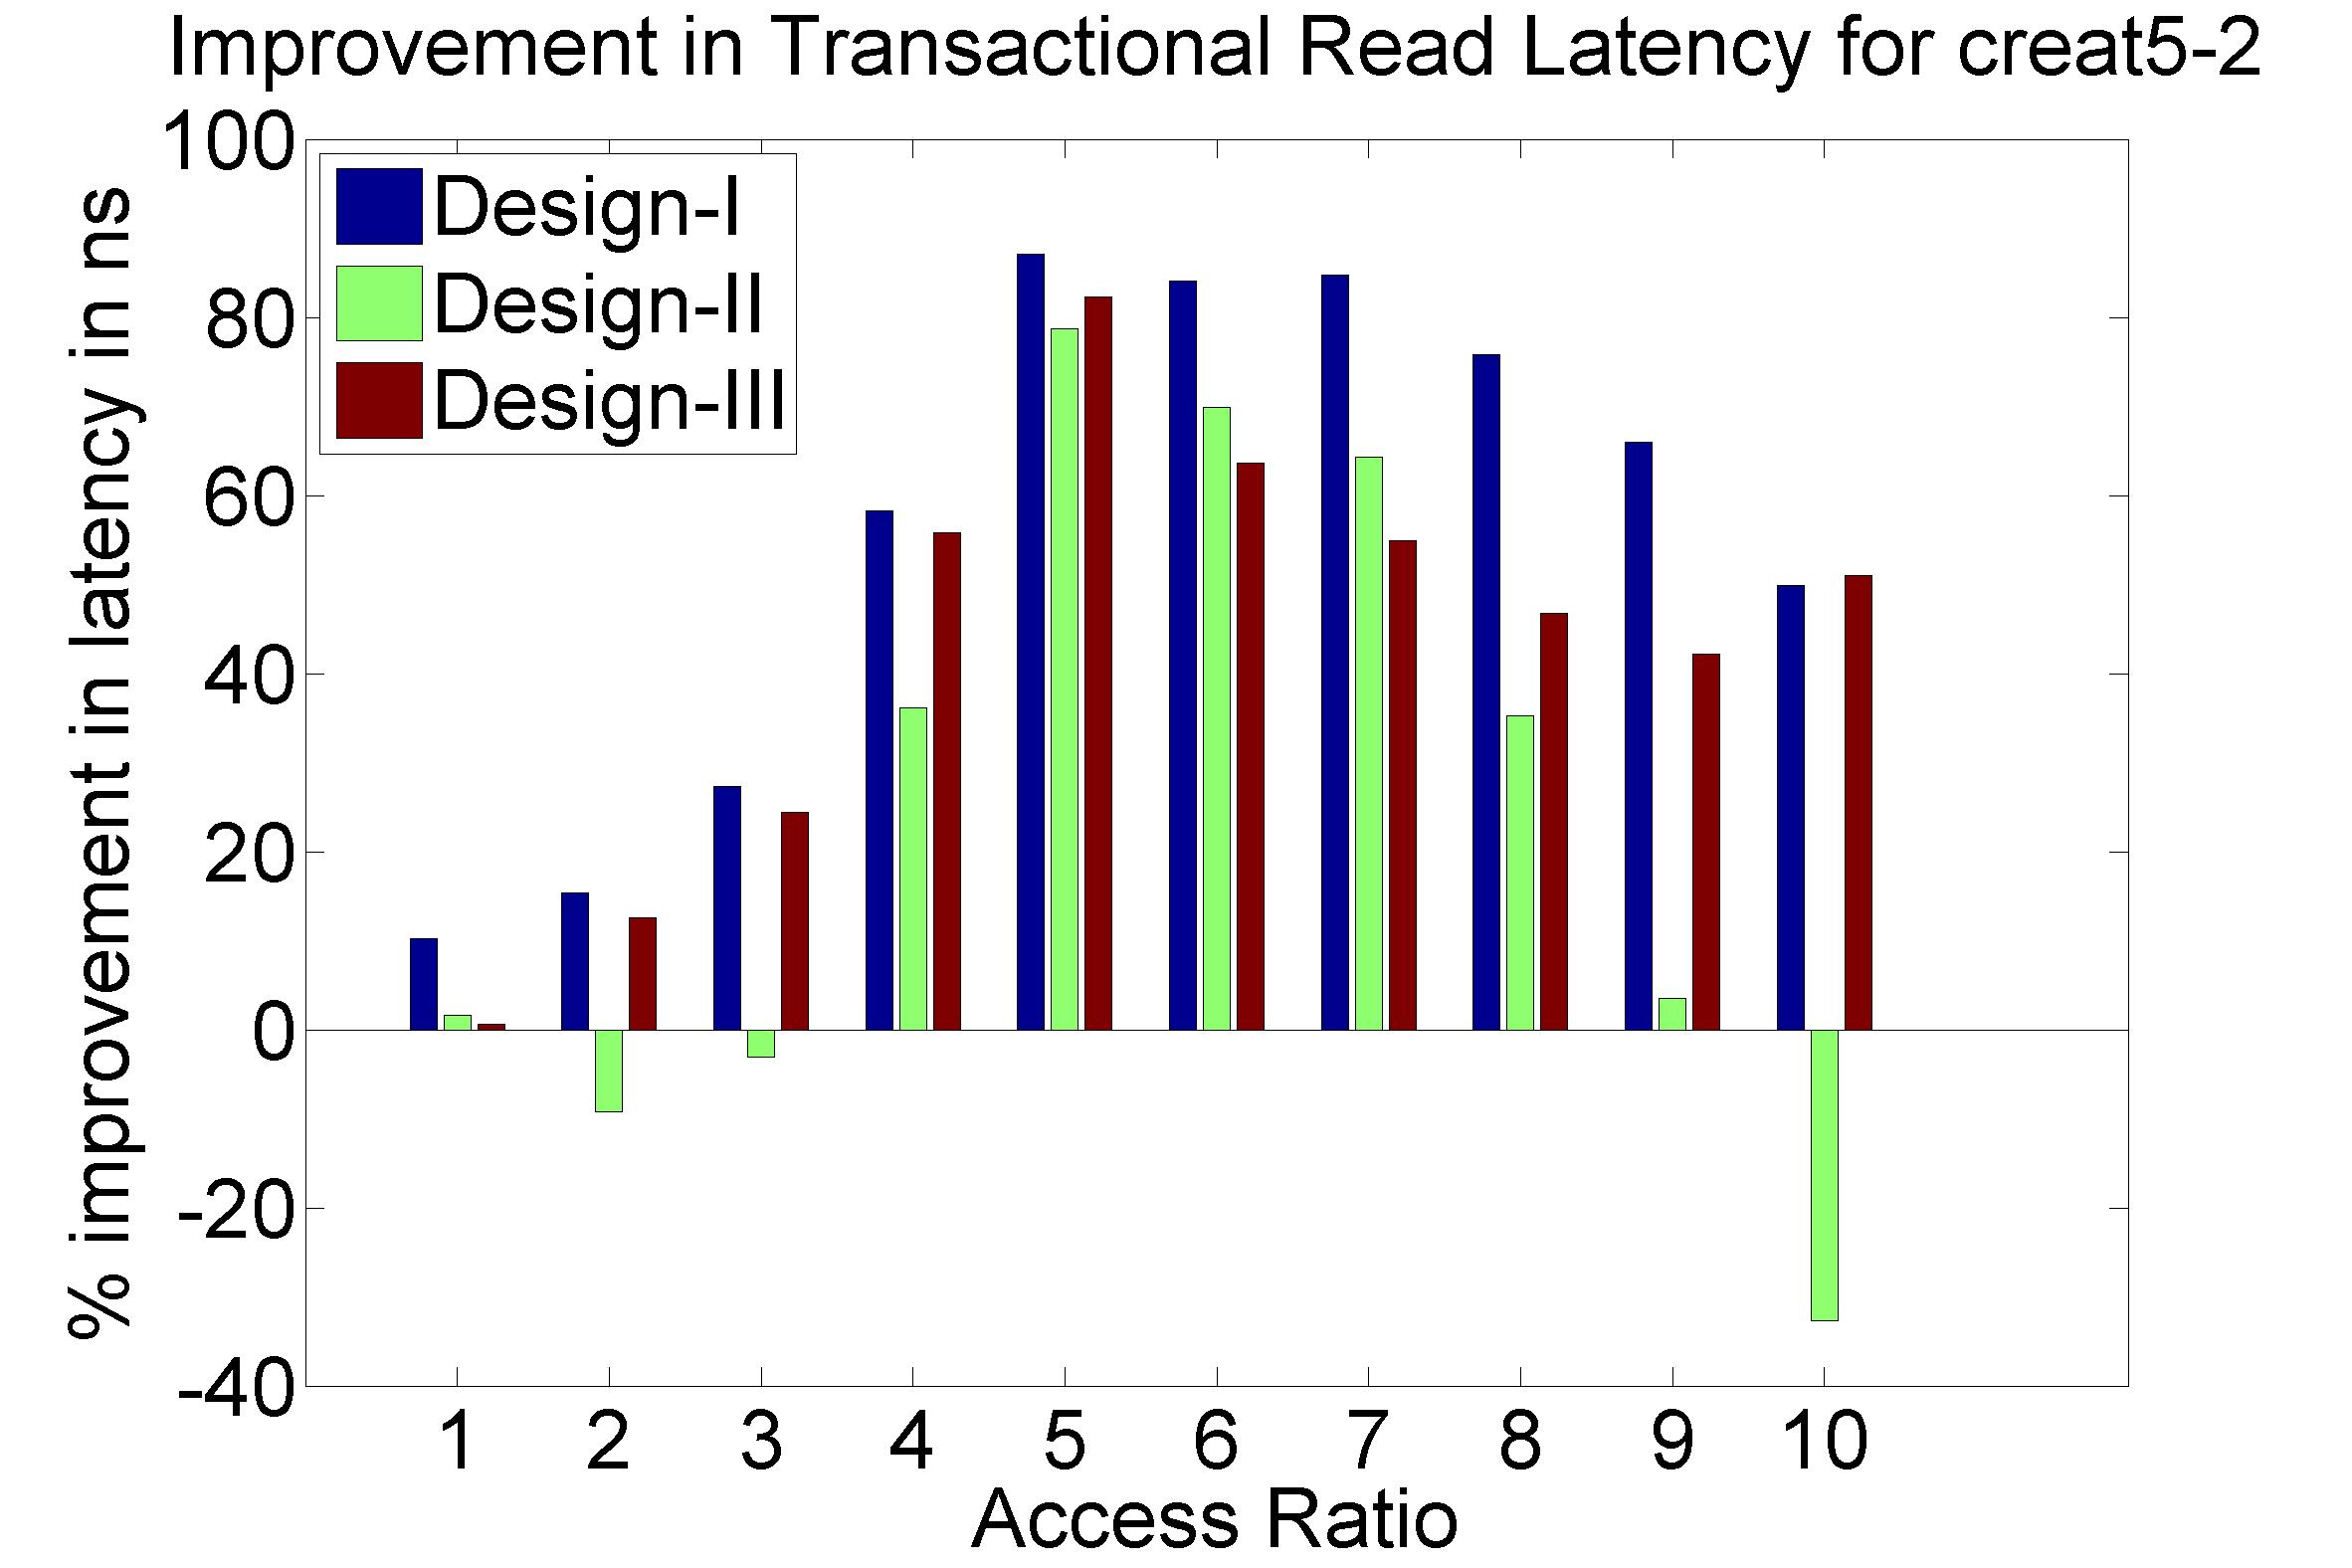
\includegraphics[width=\linewidth]{creat5-2_transactional_latency_improvement.jpeg}
\end{minipage}
\begin{minipage}[!t]{0.32\linewidth}
        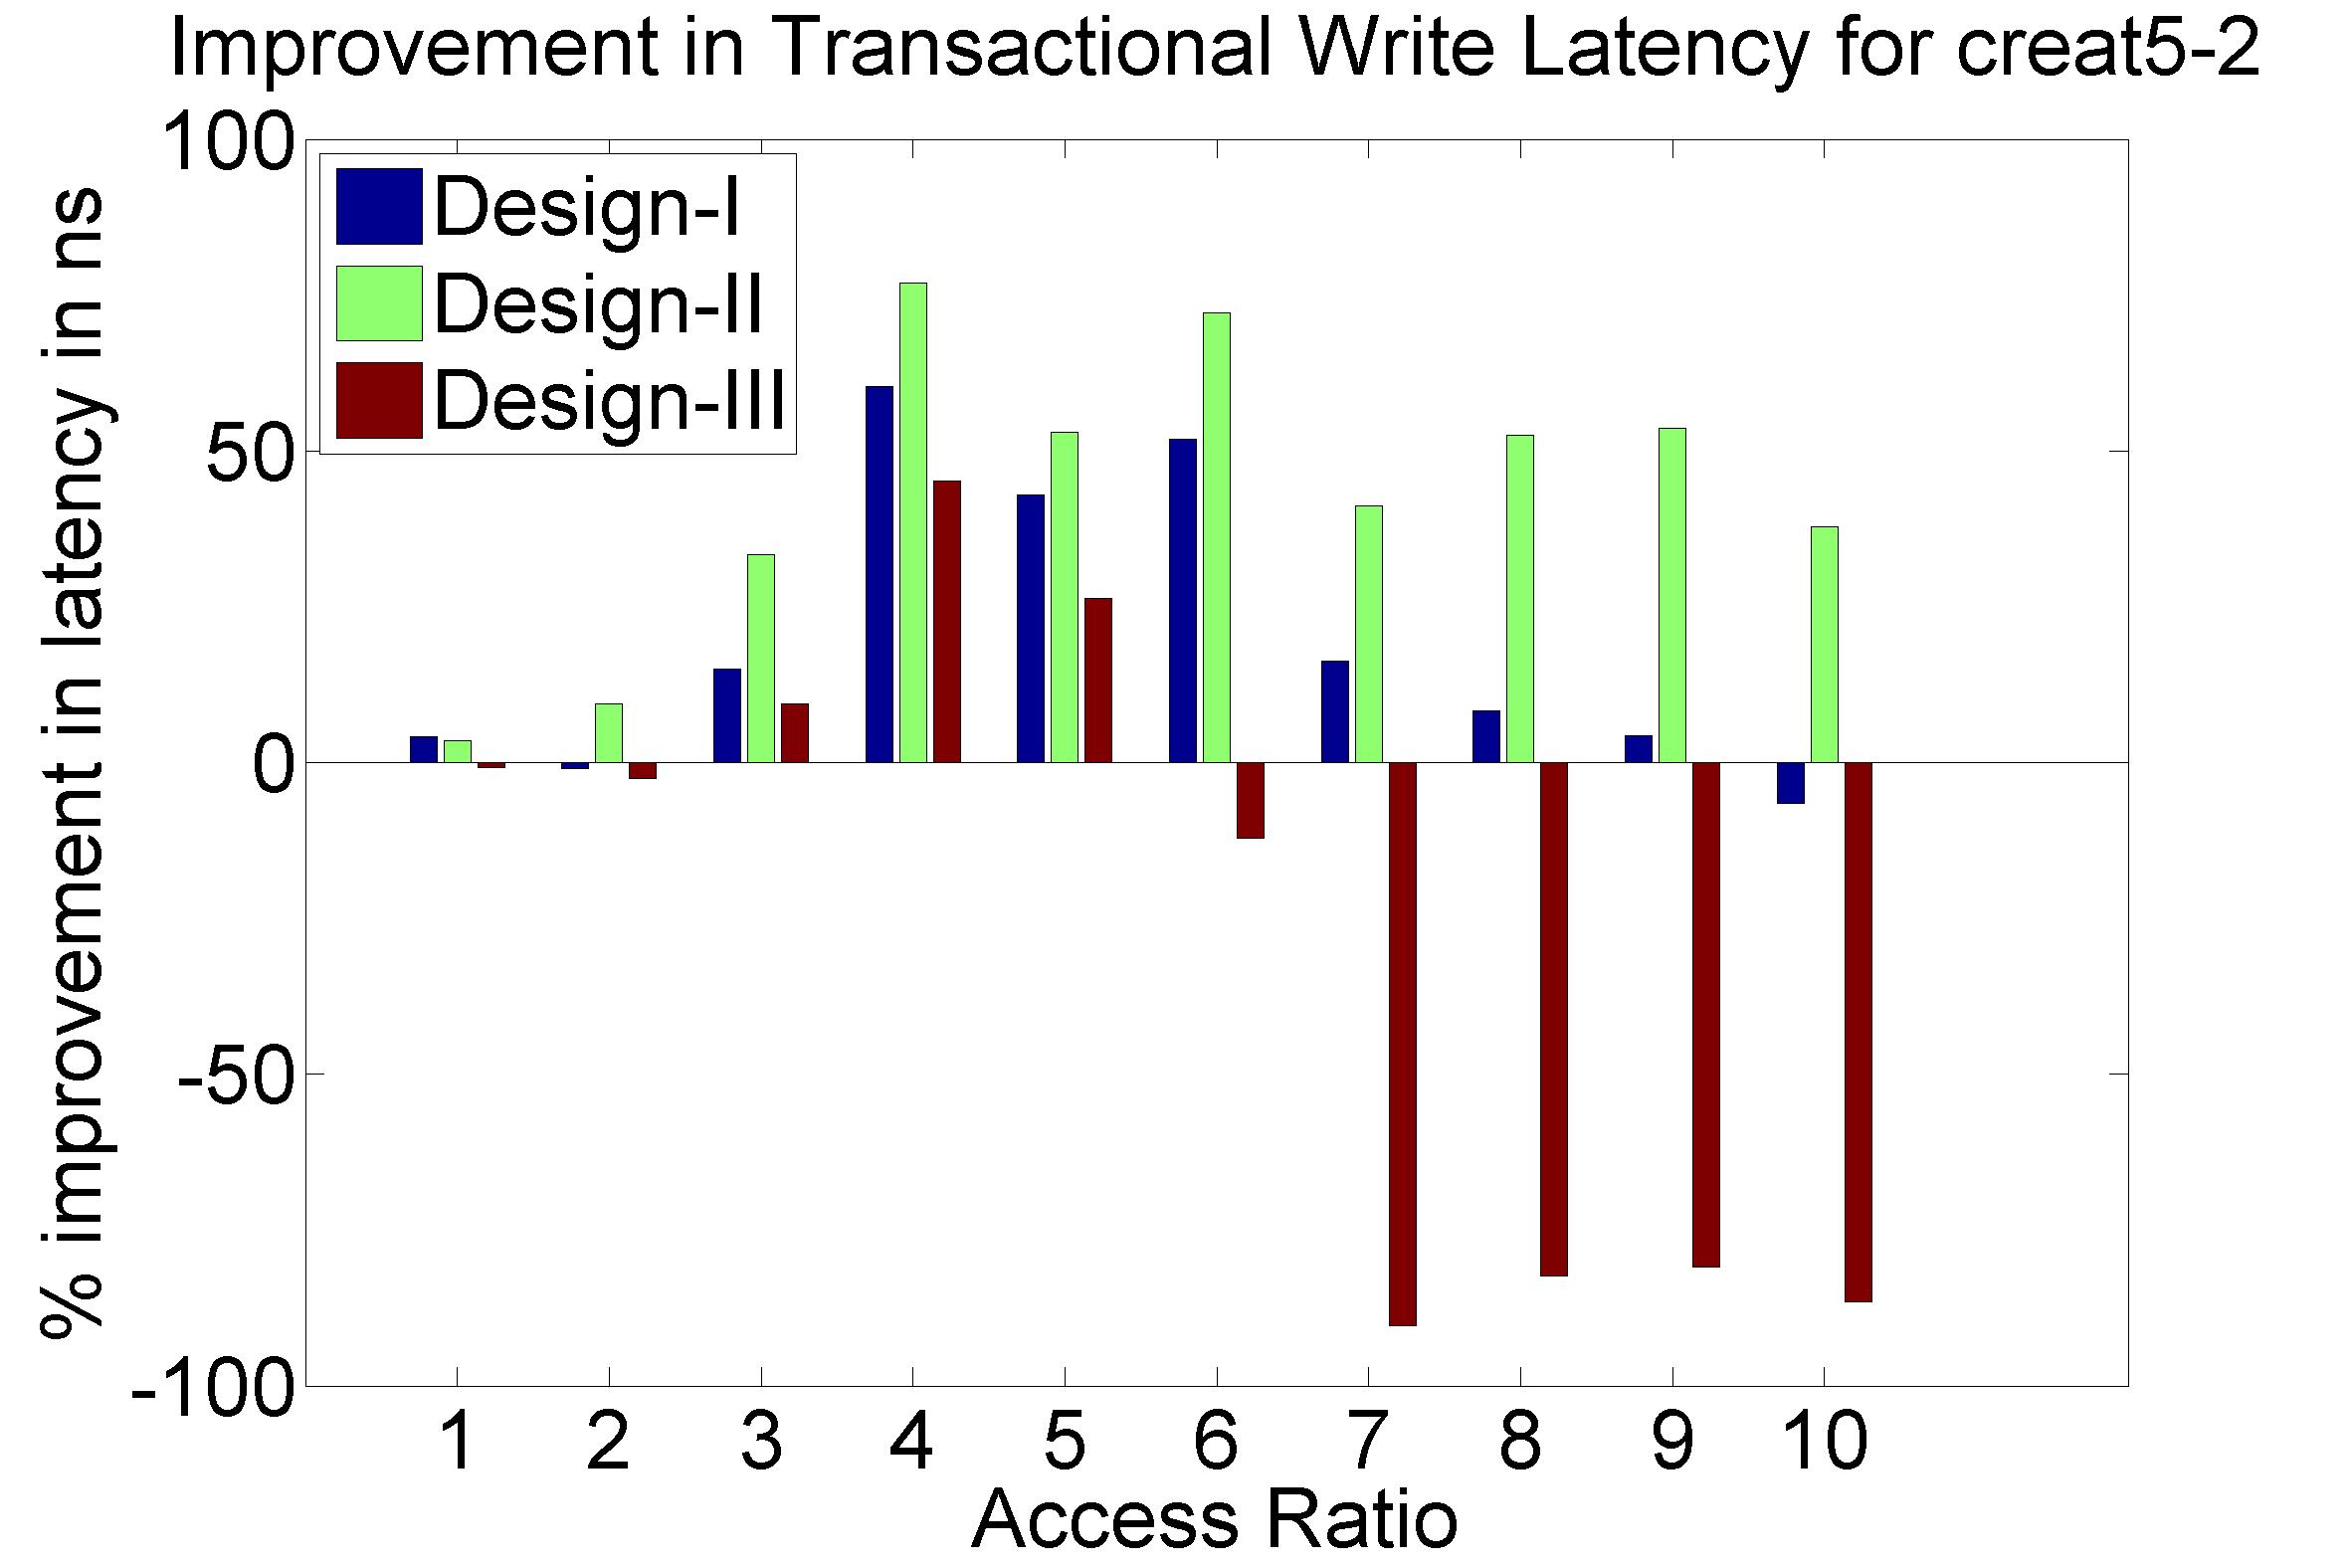
\includegraphics[width=\linewidth]{creat5-2_write_latency_improvement.jpeg}
\end{minipage}
\caption{
{\bf Performance Graphs for Creat5-2 trace} }
\label{fig:creat52_improvement}
\end{figure}
%-------------------------------------------------
Observations : 
\begin{itemize}
	\item Creat5-2 is a part of Creat5 trace. Creat5-2 is a high density trace. 
	\item There is a significant critical read latency improvement for all access ratios in all design. 
	\item The transactional read latency improves for all access ratios.
	\item The write access latency improves for ratios between 3 and 6.
 	\item All the code designs are ideal for this trace. 
	\item Coding architecture is ideal for this trace.
\end{itemize}
\cleardoublepage
{\bf Conclusions}
\begin{itemize}
	\item Table~\ref{table:perfImprovementComparison} summarizes improvement across all traces. 
	\item The systemC simulation of proposed algorithms considers benefit of coding with cost. 
	\item The Coding architecture performs at its best when the trace density is {\em High}. For e.g., Creat5-1 and Creat5-2.
	\item Design I,II and III have associated costs according to table~\ref{table:codedesigncomparison}.
	\item Access Ratio is defined as $\frac{\text{speed of cores in ns}}{\text{speed of memory in ns}}$
\end{itemize}
\begin{table}[tbp]
	\centering
	\begin{tabular}{|c|c|p{4cm}|p{4.2cm}|p{4.2cm}|p{3.3cm}|p{3.3cm}| }
\hline
Trace & Density & Critical Read Latency Improvement & Transactional Read Latency Improvement & Transactional Write Latency Improvement & Access ratio with 15-20$\%$ improvement for Read & Access ratio with 15-20$\%$ improvement for Write\\
% Design & 
\hline
\hline
LTE & Medium &Varies from  -10 to 80$\%$ & Varies from -50 to 80$\%$ & Varies from -150 to 300$\%$ & access ratio 4 to 10 & access ratio 3 to 6 \\
\hline 
UMTS & Medium &Varies from   -5 to 90$\%$ & Varies from 0 to 80$\%$ & Varies from -150 to 150 $\%$ & access ratio 2 to 6 & access ratio 3 to 5 \\
\hline
Case4 & Low &Varies from 1 to 14$\%$ & Varies from -20 to 25$\%$ & Varies from -0.2 to 0.4 $\%$ & access ratio 5 to 10 & None \\
\hline
Creat4-1 & Medium &Varies from 0 to 80$\%$ & Varies from -100 to 80$\%$ & Varies from -15 to 5 $\%$ & access ratio 4 to 10 & access ratio 5 to 6\\
\hline
Creat4-2 & Medium &Varies from -5 to 60$\%$ & Varies from -80 to 60$\%$ & Varies from -17 to 8 $\%$ & access ratio 4 to 10 & None \\
\hline
Creat5-1 & High &Varies from 5 to 95$\%$ & Varies from 5 to 90$\%$ & Varies from -60 to 55 $\%$ & access ratio 2 to 10 & access ratio 3 to 6 \\
\hline
Creat5-2 & High &Varies from 10 to 85$\%$ & Varies from -10 to 90$\%$ & Varies from 10 to 130 $\%$ & access ratio 3 to 10 & access ratio 3 to 10 \\
%\multirow{3}{*}{LTE} & I & 50-90$\%$& & \\
% & II & 50-90$\%$ & 50-90$\%$ & \\
%& III & & & \\
%\multirow{3}{*}{UMTS} & I & & & \\
% & II & & & \\
% & III & & & \\
%\multirow{3}{*}{Case4} & I & & & \\
% & II & & & \\
% & III & & & \\
%Creat4-1 & 0 to 90$\%$ & -30 to 90$\%$ & 15-400 $\%$ \\
%\multirow{3}{*}{Creat4-1} & I & & & \\
% & II & & & \\
% & III & & & \\
%Creat4-2 & 0 to 90$\%$ & -30 to 90$\%$ & 15-400 $\%$ \\
%\multirow{3}{*}{Creat4-2} & I & & & \\
% & II & & & \\
% & III & & & \\
%Creat5-1 & 0 to 90$\%$ & -30 to 90$\%$ & 15-400 $\%$ \\
%\multirow{3}{*}{Creat5-1} & I & & & \\
% & II & & & \\
% & III & & & \\
%Creat5-2 & 0 to 90$\%$ & -30 to 90$\%$ & 15-400 $\%$ \\
%\multirow{3}{*}{Creat5-2} & I & & & \\
% & II & & & \\
% & III & & & \\
\hline
\end{tabular}
\caption{Performance Improvement Comparison Table}
\label{table:perfImprovementComparison}
\end{table}
\end{landscape}
\cleardoublepage
\pagestyle{fancy}

